\documentclass[10pt]{beamer}
%Information to be included in the title page:
\title{Taller de Supervivencia en Shell}
\author{Robotech}
\institute{URJC}
\date{2023}
\usetheme{Madrid}
\usecolortheme{beaver}
\usepackage{graphicx} %LaTeX package to import graphics
\graphicspath{{images/}} %configuring the graphicx package
\logo{
\includegraphics[width=0.25\textwidth]{logo}
\includegraphics[scale=0.2]{robotech}}

\begin{document}
	
	\frame{\titlepage}
	
	\begin{frame}
		\frametitle{Licencia}
		(cc) 2018 Grupo de Sistemas y Comunicaciones.
		\newline
		\newline
		(cc) 2023 Robotech.
		\newline
		\newline
		Algunos derechos reservados. Este trabajo se entrega bajo la licencia Creative Commons Reconocimiento –NoComercial - SinObraDerivada (by-nc-nd). Para obtener la licencia completa, véase:
		\newline
		\newline
		http://creativecommons.org/licenses/by-sa/2.1/es.También puede solicitarse a Creative Commons, 559 Nathan
		\newline
		\newline
		Abbott Way, Stanford, California 94305, USA.
	\end{frame}
	
	\begin{frame}
		\frametitle{¿Quiénes somos?}
		\begin{itemize}
			\item Javier Izquierdo Hernández: \\
			Estudiante de ingeniería robótica software (3º año).
			\item Iker Peral del Pino: \\
			Estudiante de ingeniería robótica software (3º año).
			\item Alguien más: \\
			Estudiante de ingeniería robótica software (3º año).
		\end{itemize}
		\vspace{20pt}
		\begin{center}
			
\includegraphics[width=15 pt]{twitter} \hspace{5 pt}
\includegraphics[width=15 pt]{instagram}\hspace{10 pt} @robotech\_urjc\\
			
			
\includegraphics[width=15 pt]{mail} \hspace{10 pt} robotechurjc@gmail.com
		\end{center}
	\end{frame}
	
	\begin{frame}
		\frametitle{¿Qué es la Shell?}
	\end{frame}

	\begin{frame}
		\frametitle{Estructura de un Comando}
	\end{frame}
	
	\begin{frame}
		\frametitle{El Manual: man}
		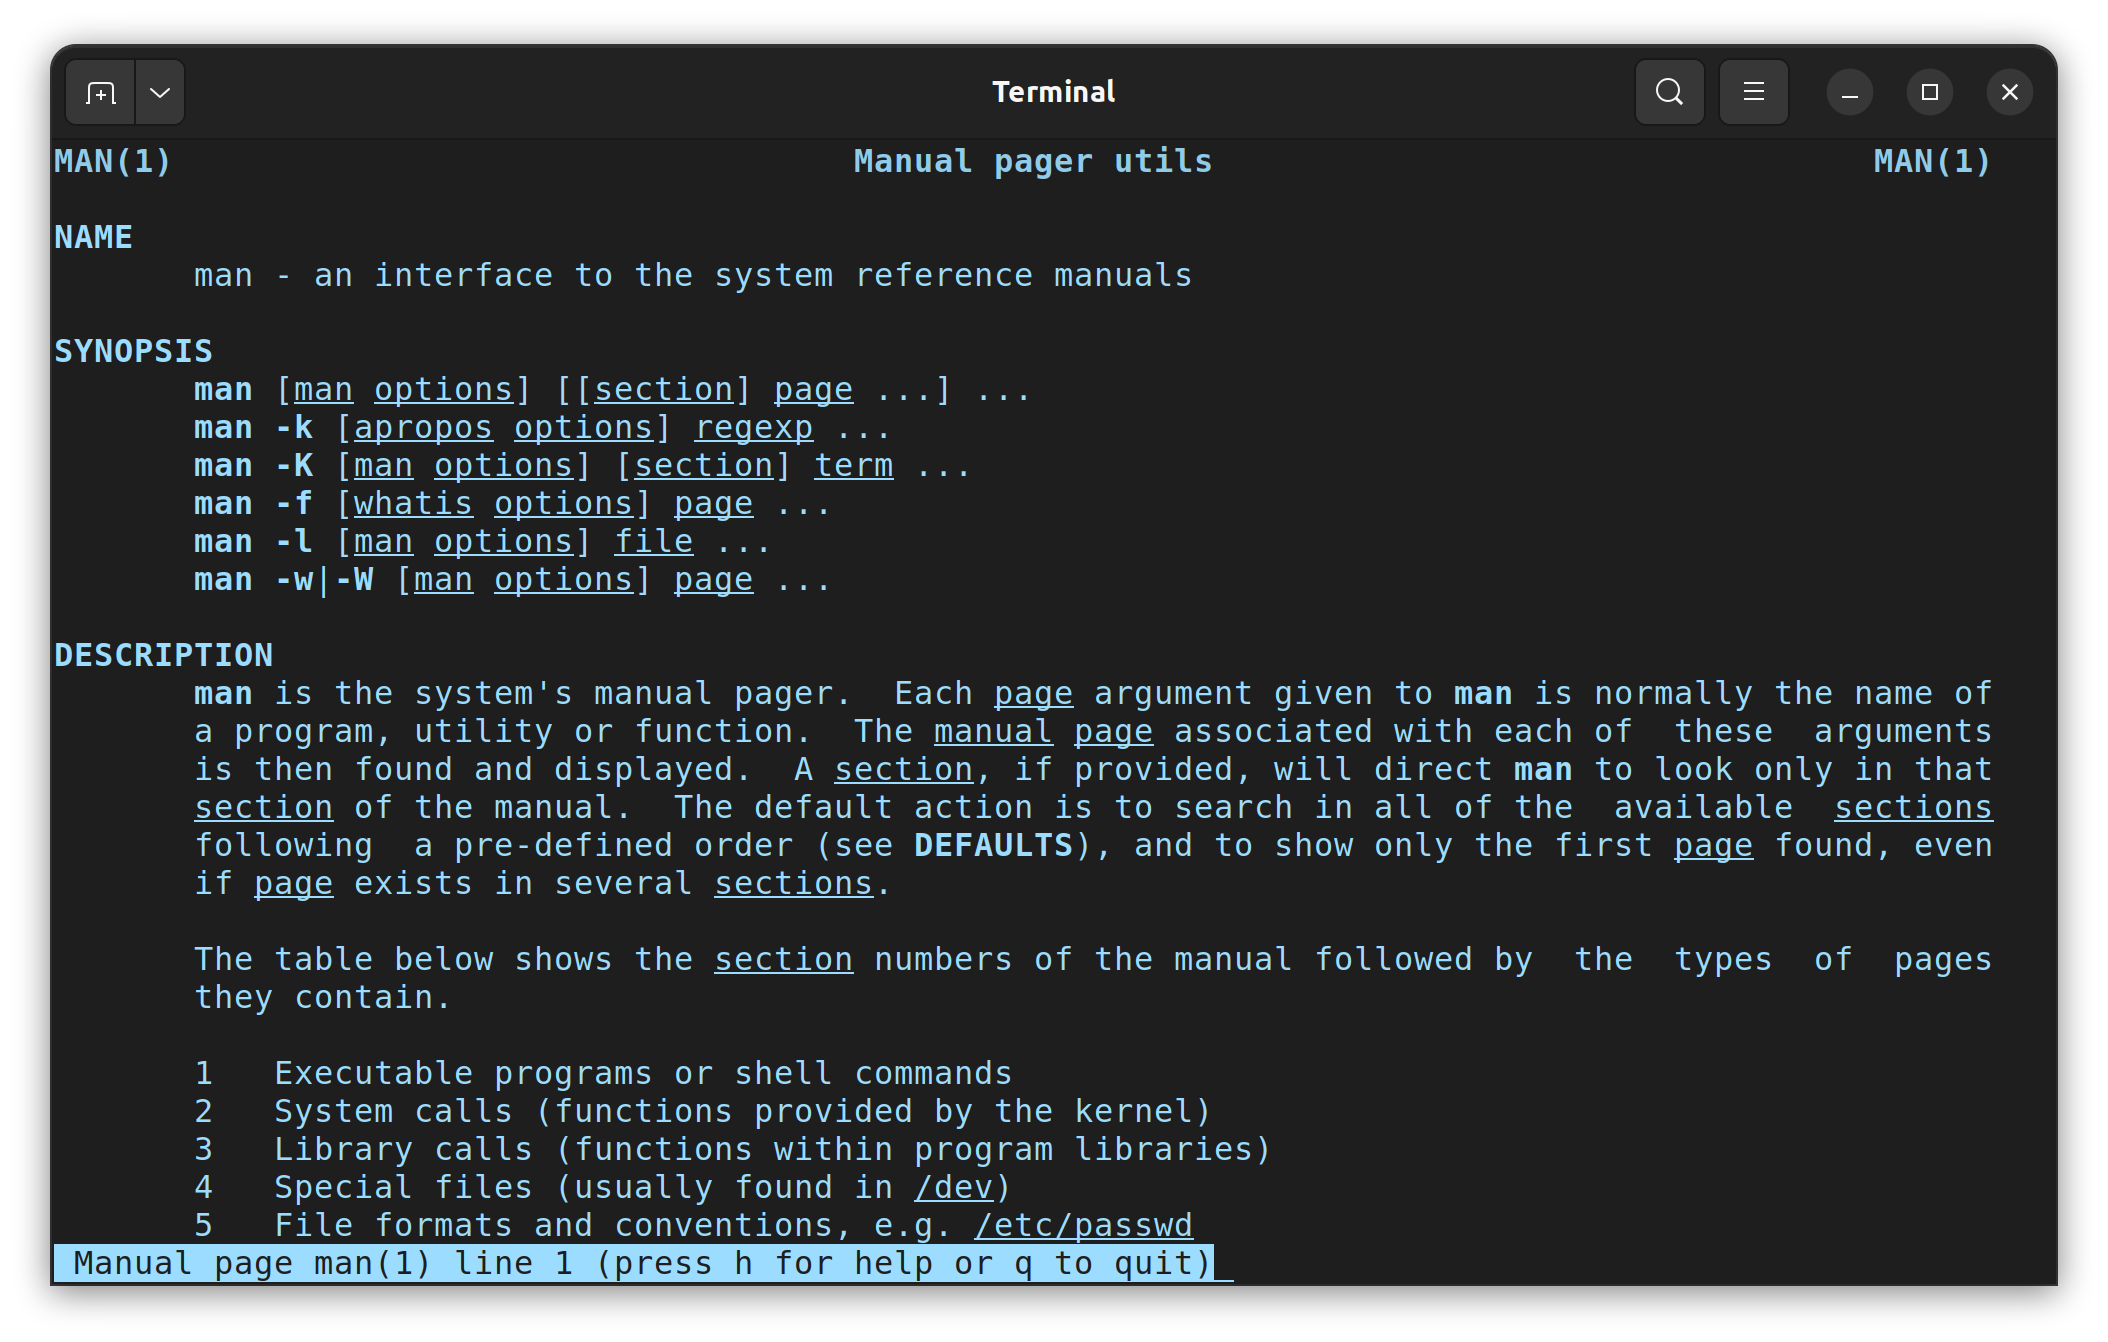
\includegraphics[width=0.75\textwidth]{man}
	\end{frame}

	\begin{frame}
		\frametitle{Primeros compandos: date}
		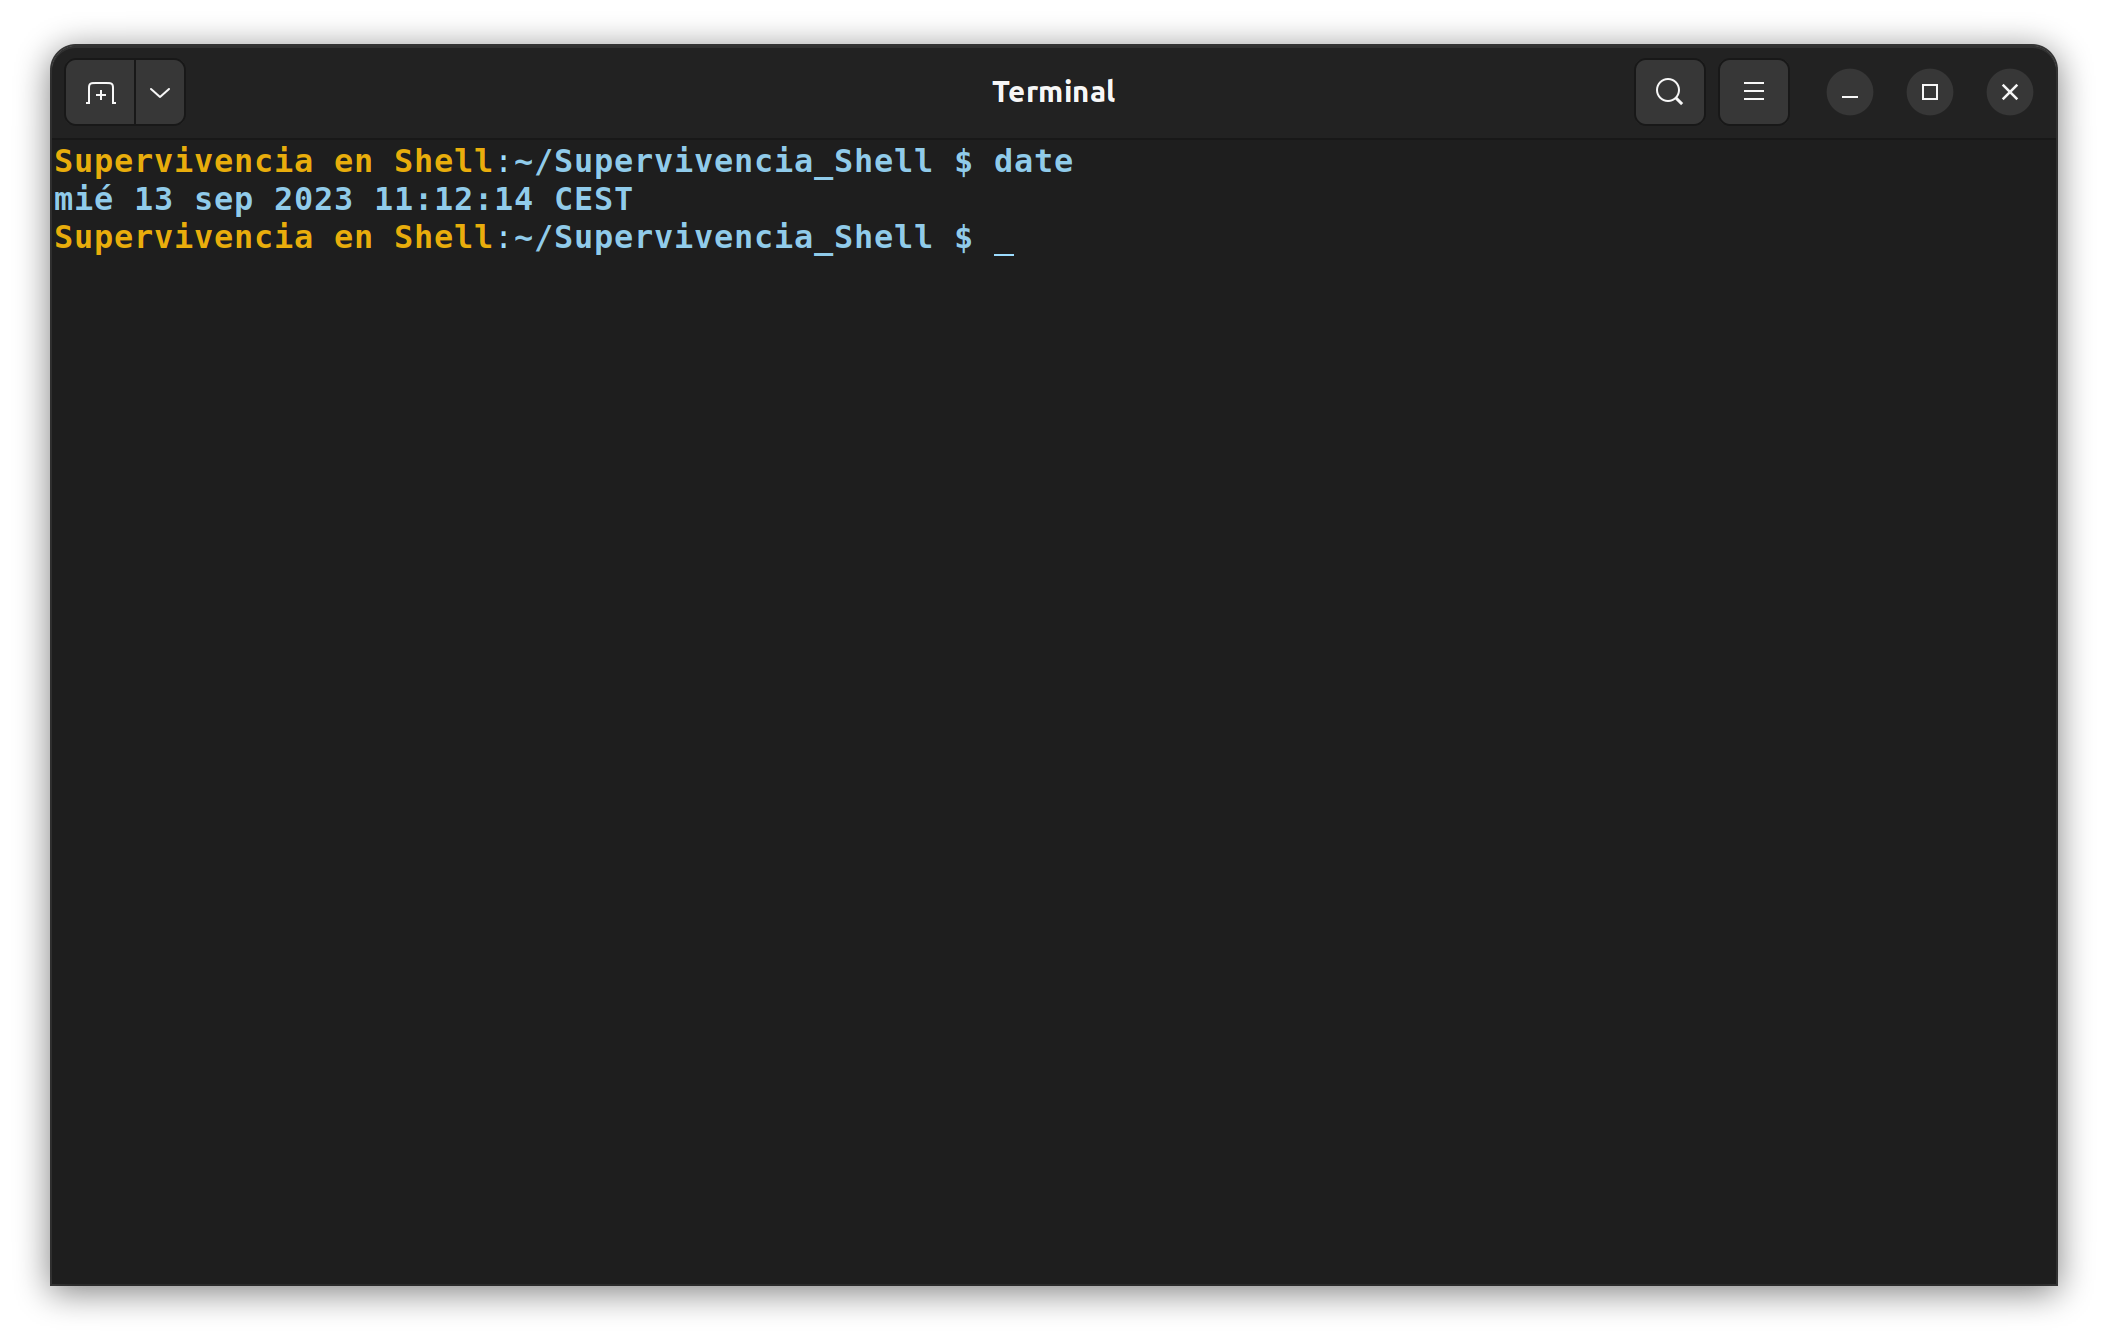
\includegraphics[width=0.75\textwidth]{date}
	\end{frame}
	
	\begin{frame}
		\frametitle{Primeros compandos: who}
		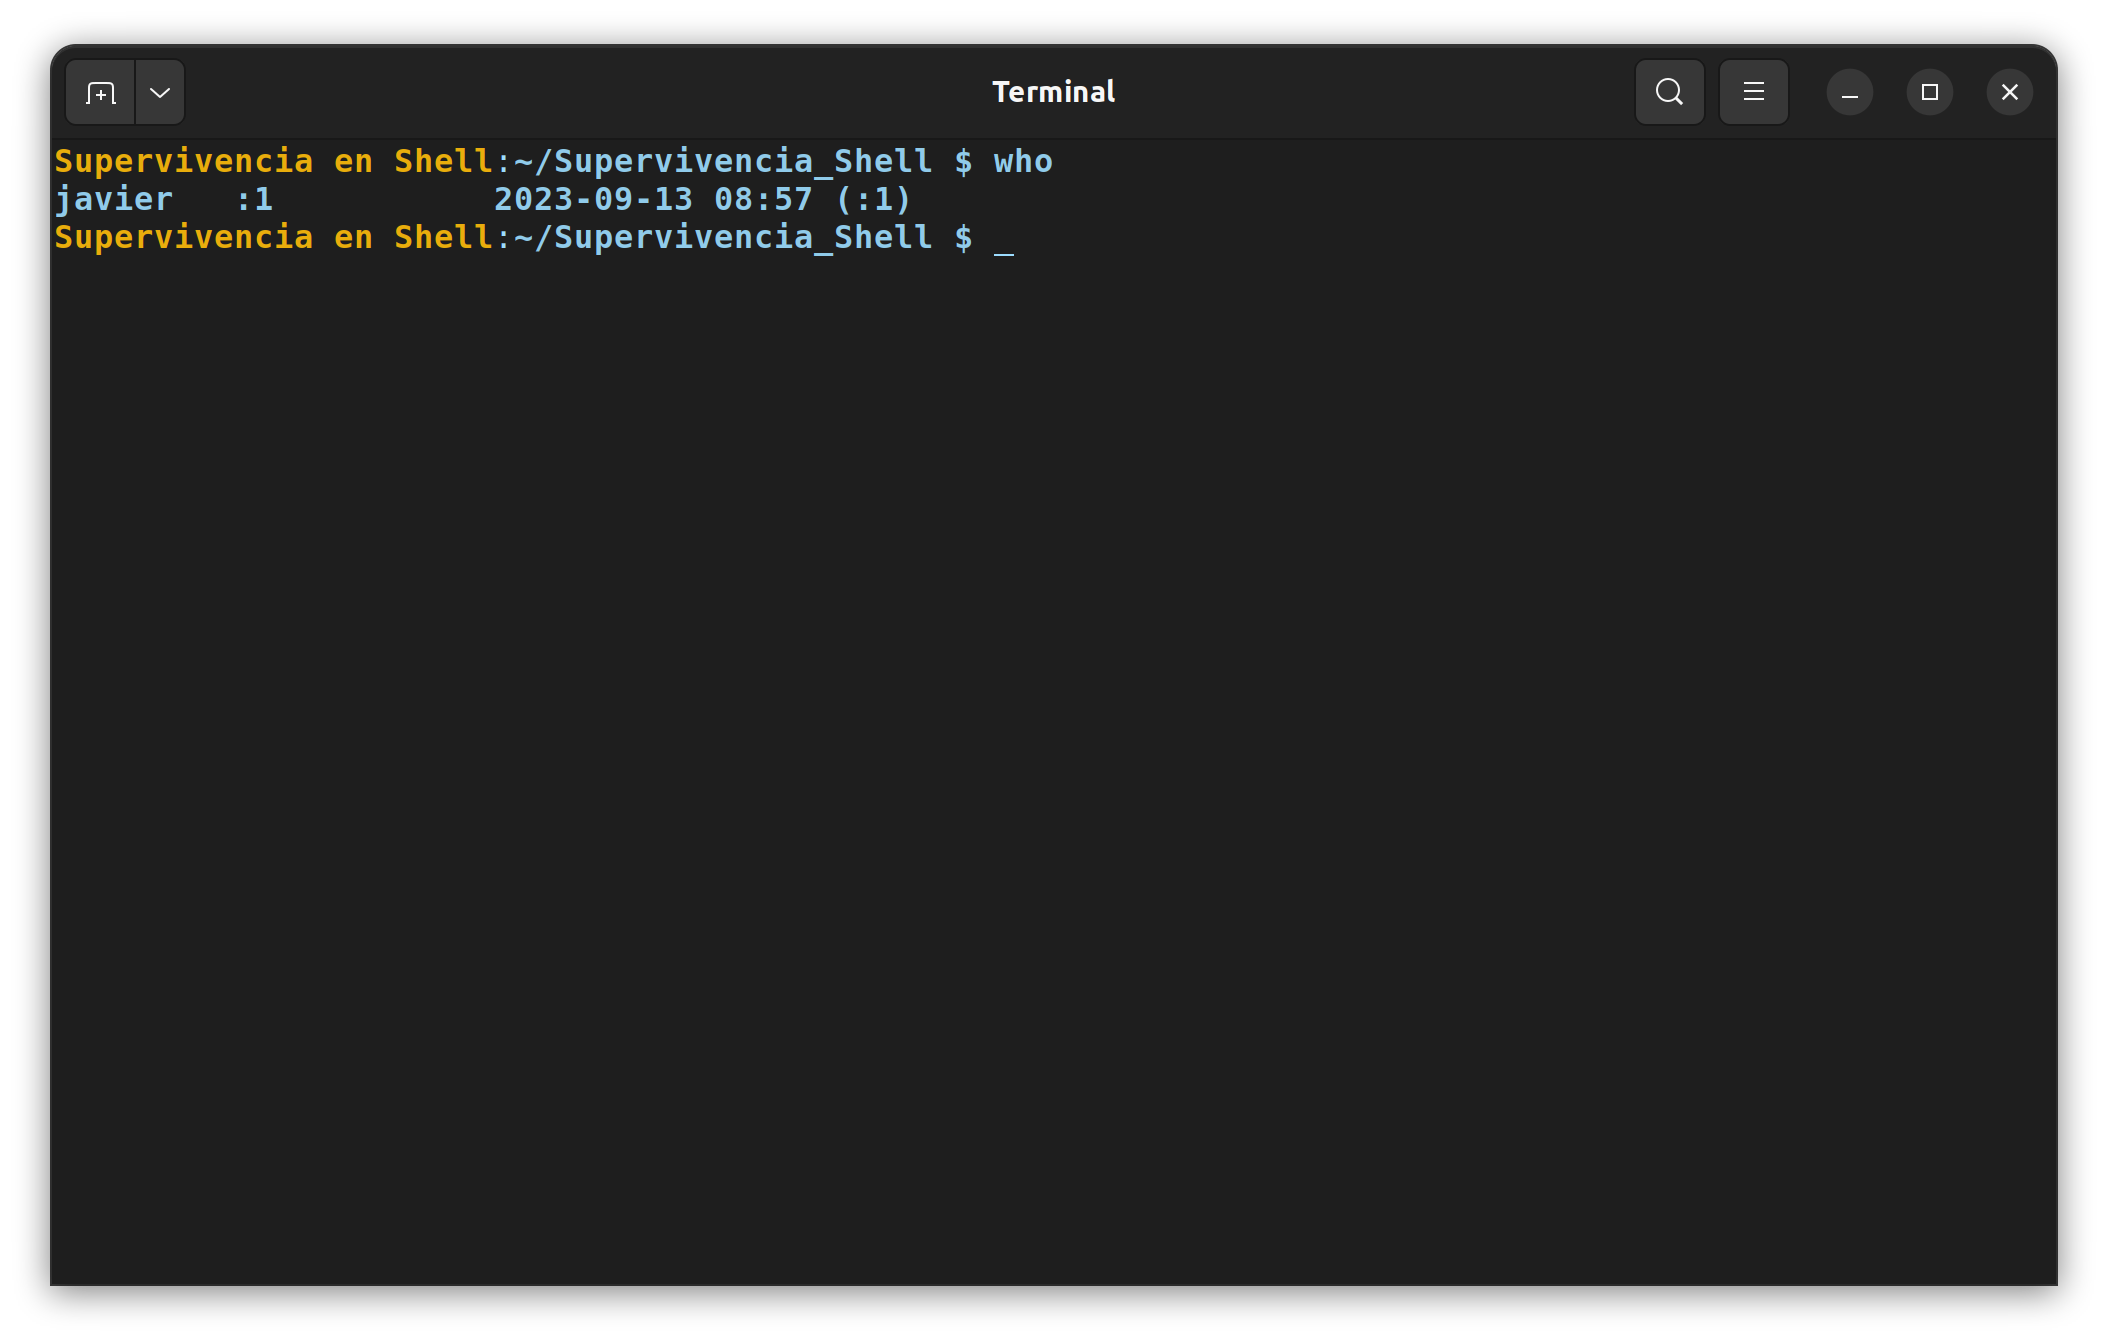
\includegraphics[width=0.75\textwidth]{who}
	\end{frame}
	
	\begin{frame}
		\frametitle{Primeros compandos: whoami}
		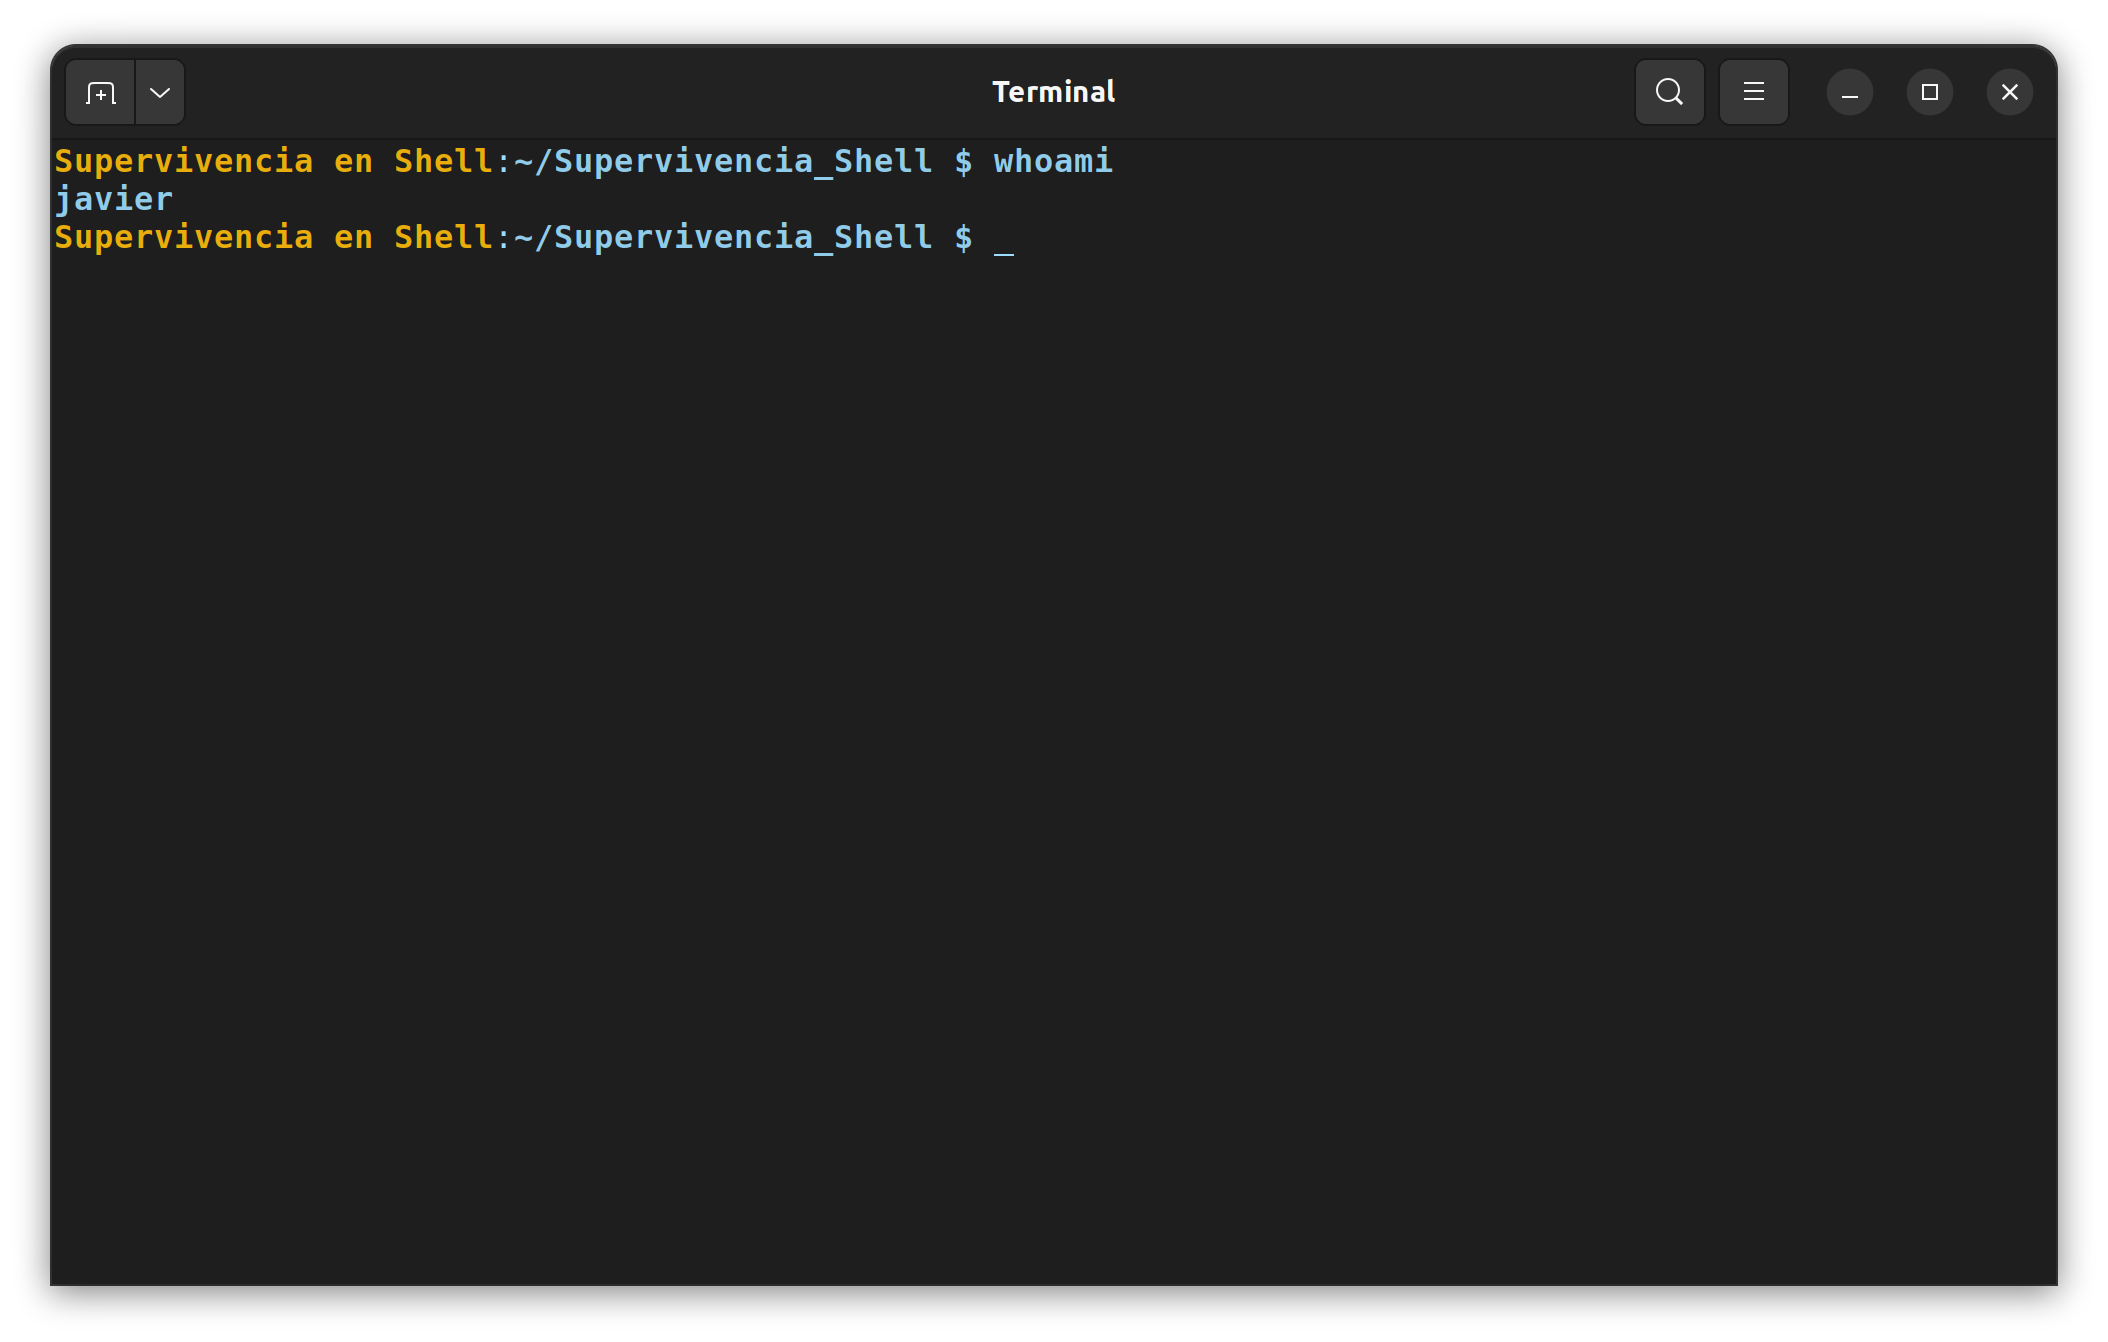
\includegraphics[width=0.75\textwidth]{whoami}
	\end{frame}
	
	\begin{frame}
		\frametitle{Primeros compandos: echo}
		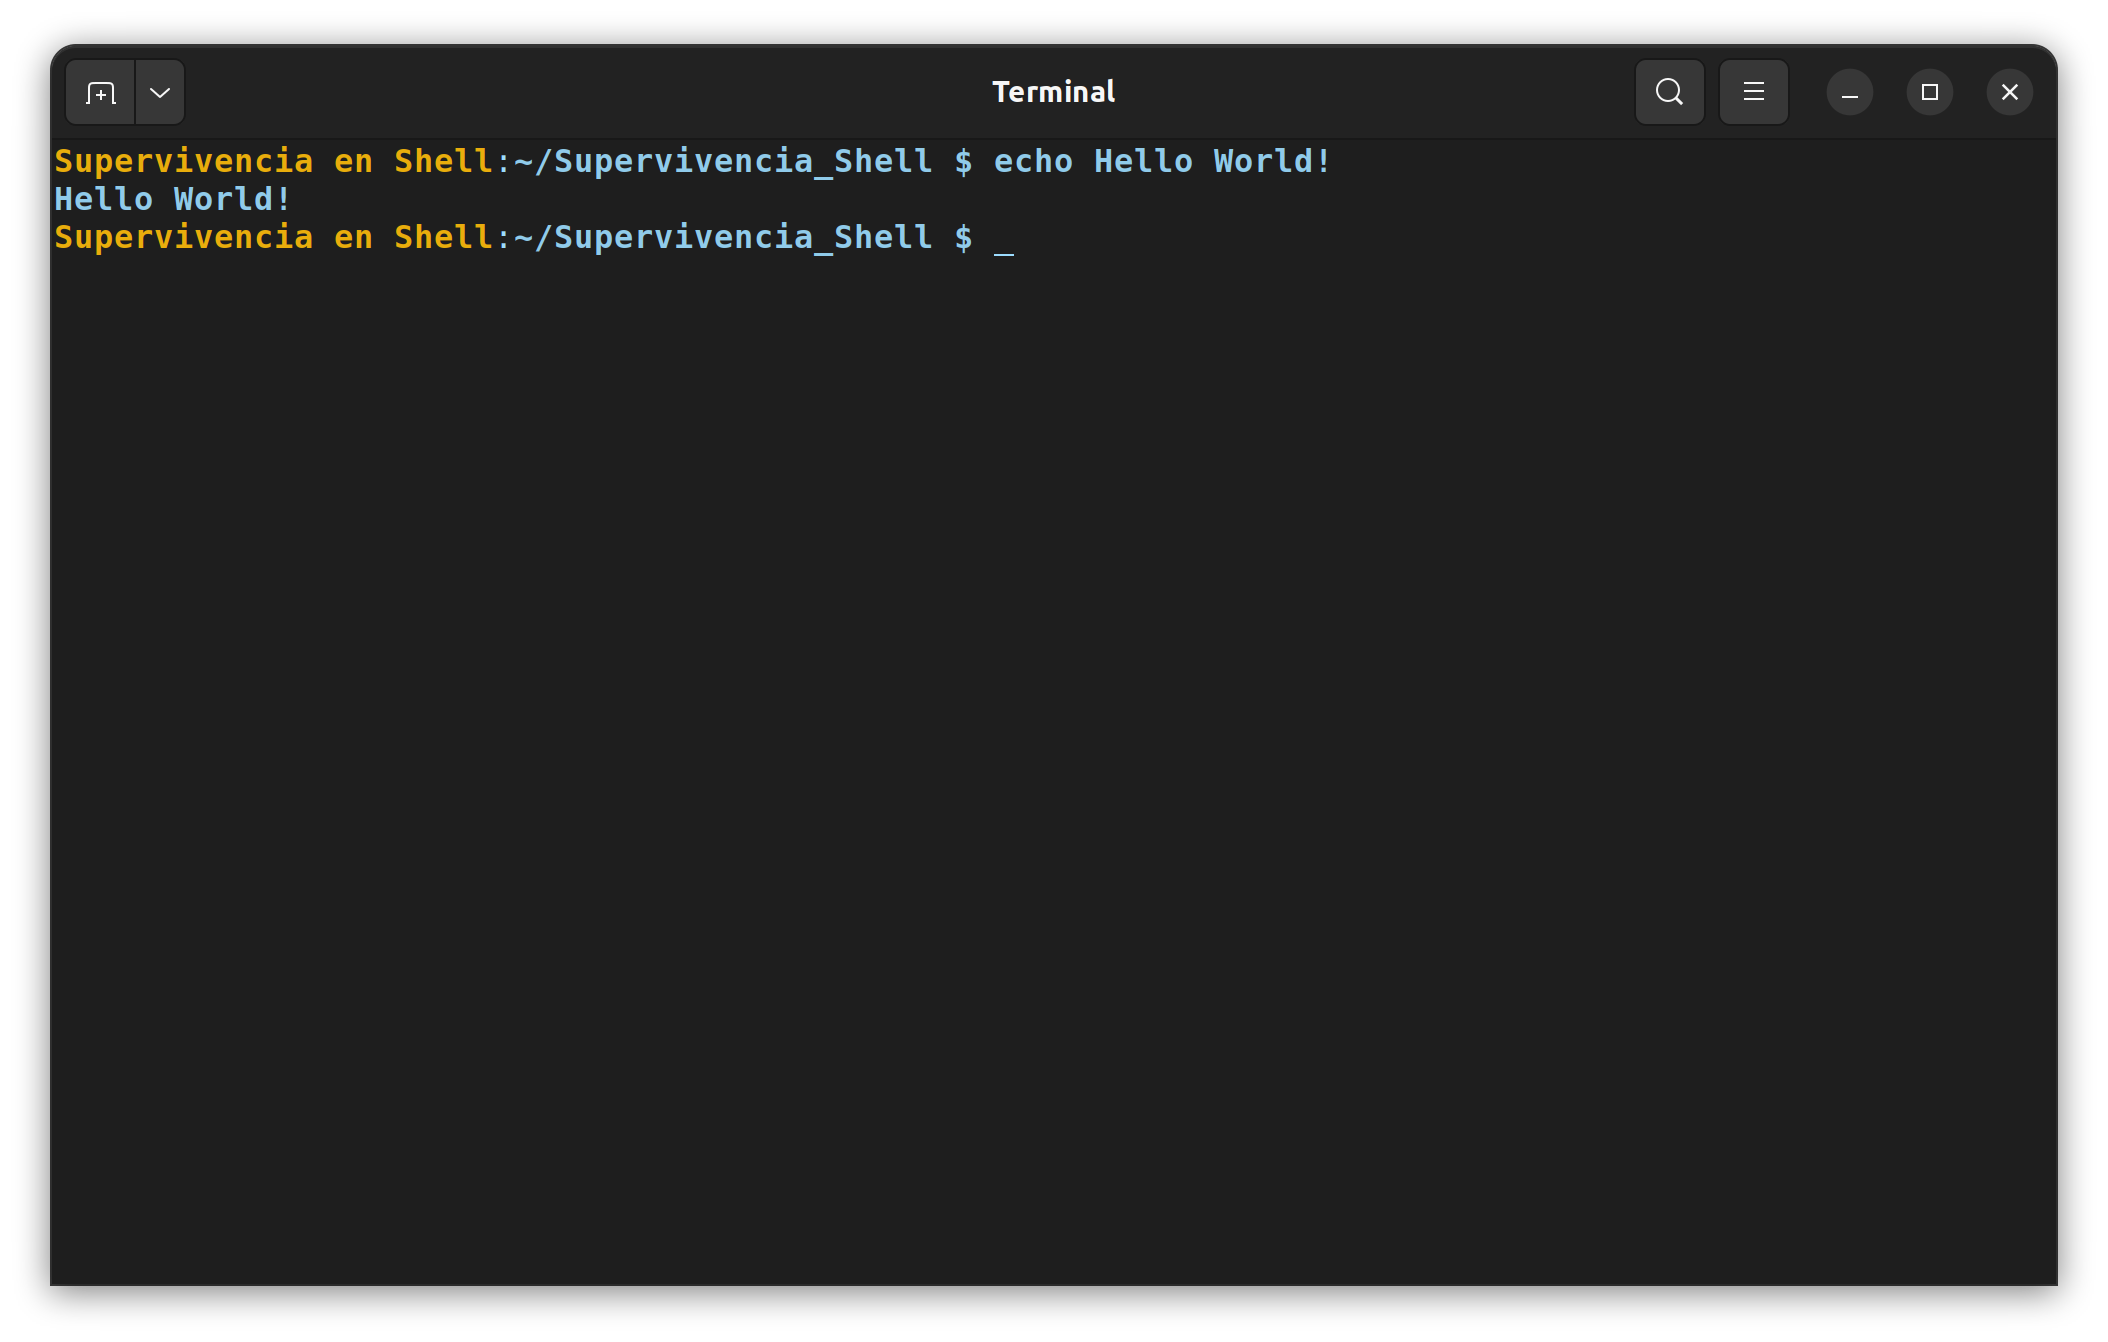
\includegraphics[width=0.75\textwidth]{echo}
	\end{frame}
	
	\begin{frame}
		\frametitle{Navegando por el terminal: ls}
		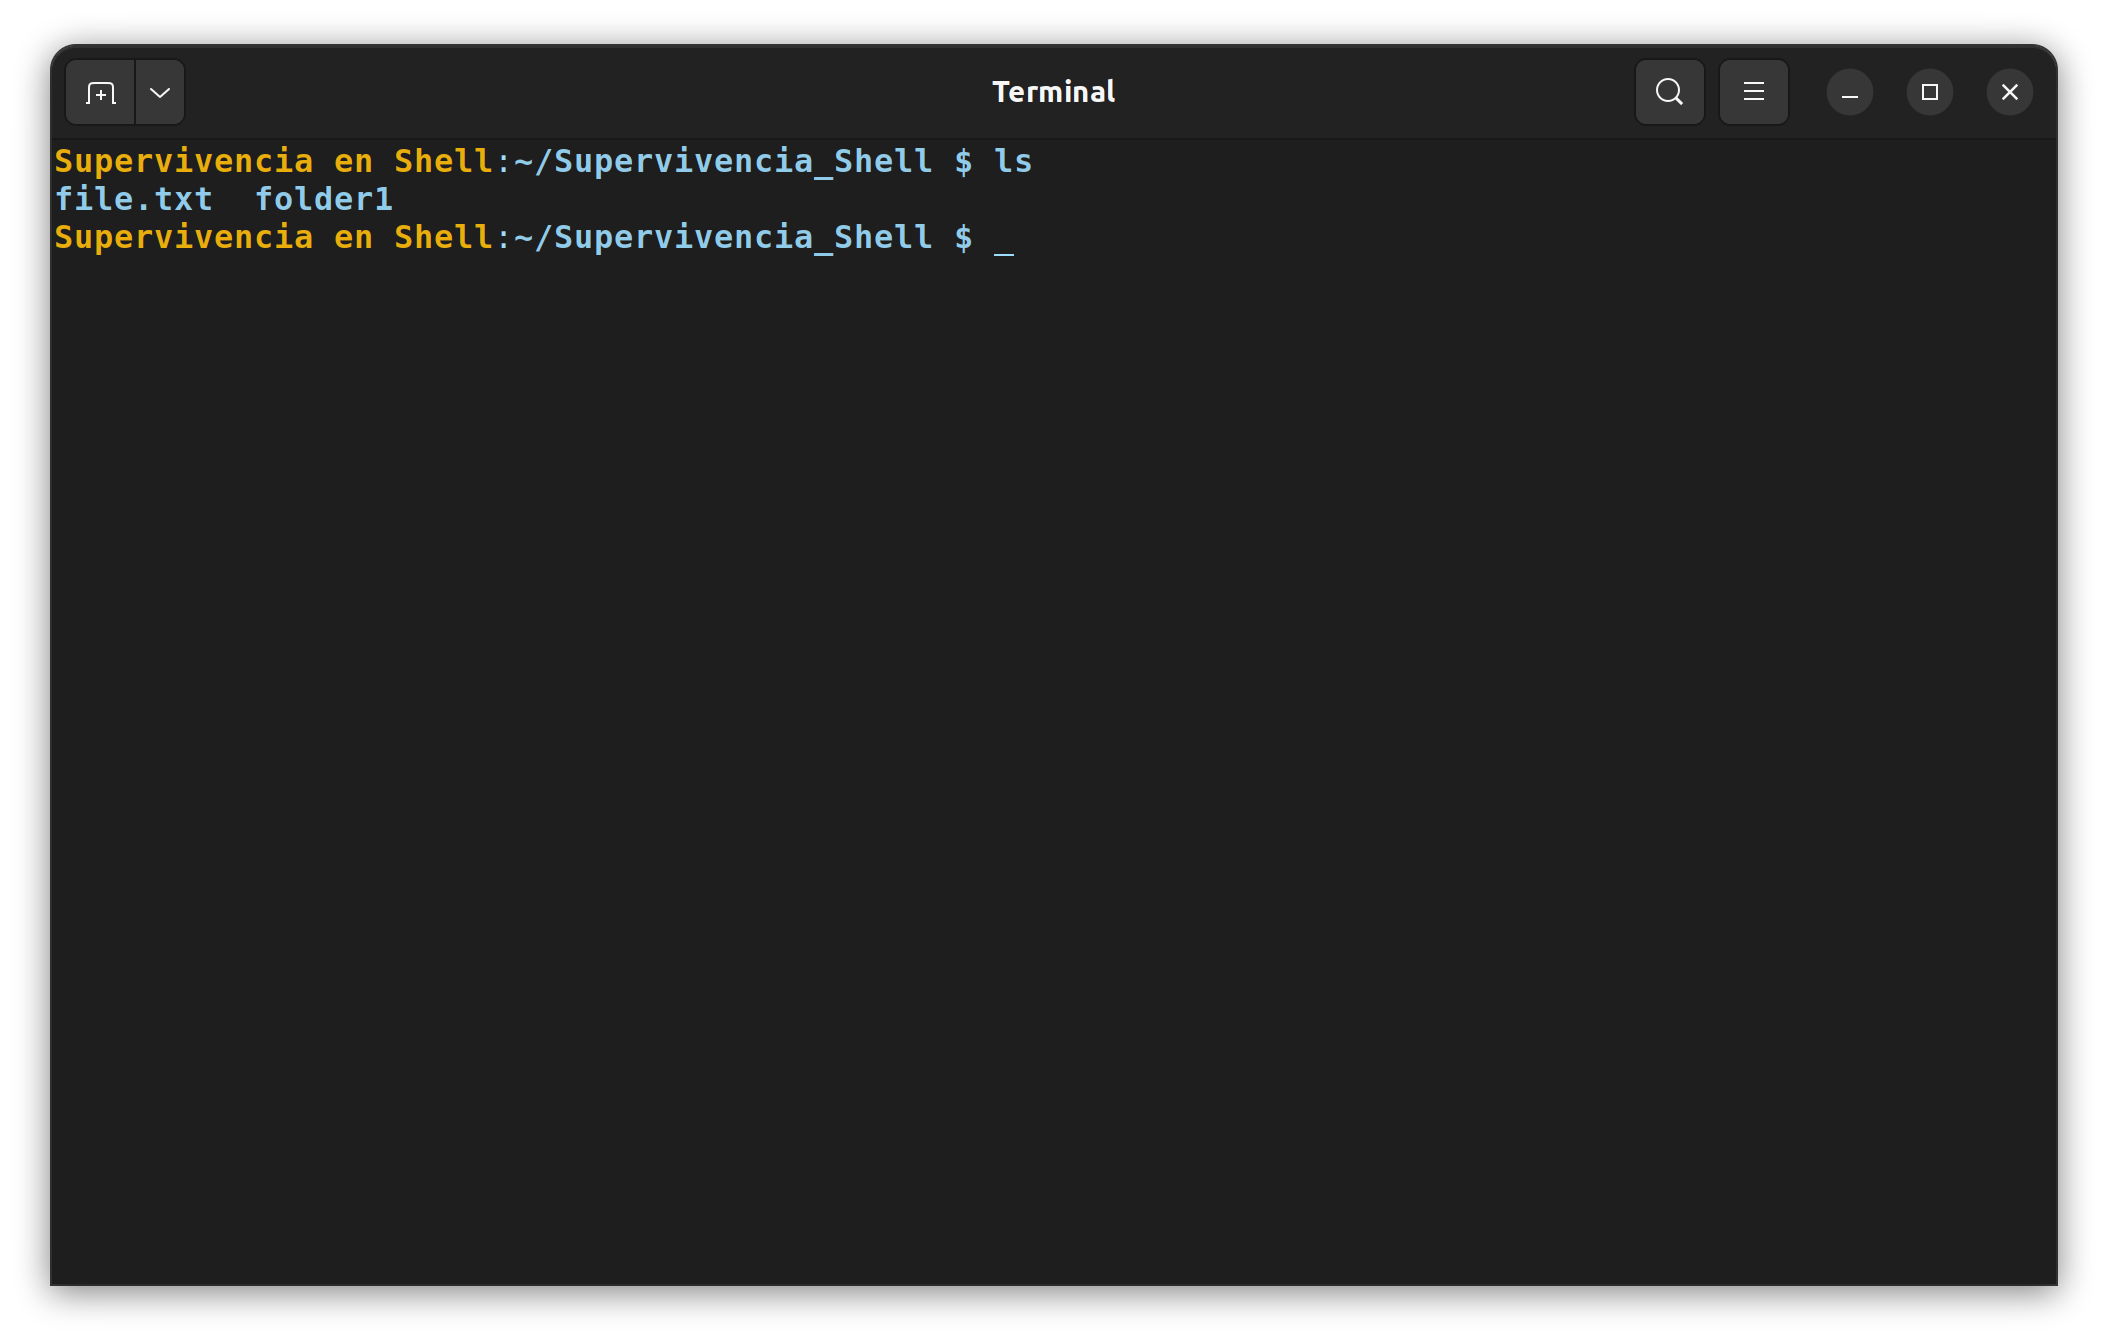
\includegraphics[width=0.75\textwidth]{ls}
	\end{frame}
	
	\begin{frame}
		\frametitle{Navegando por el terminal: cd}
		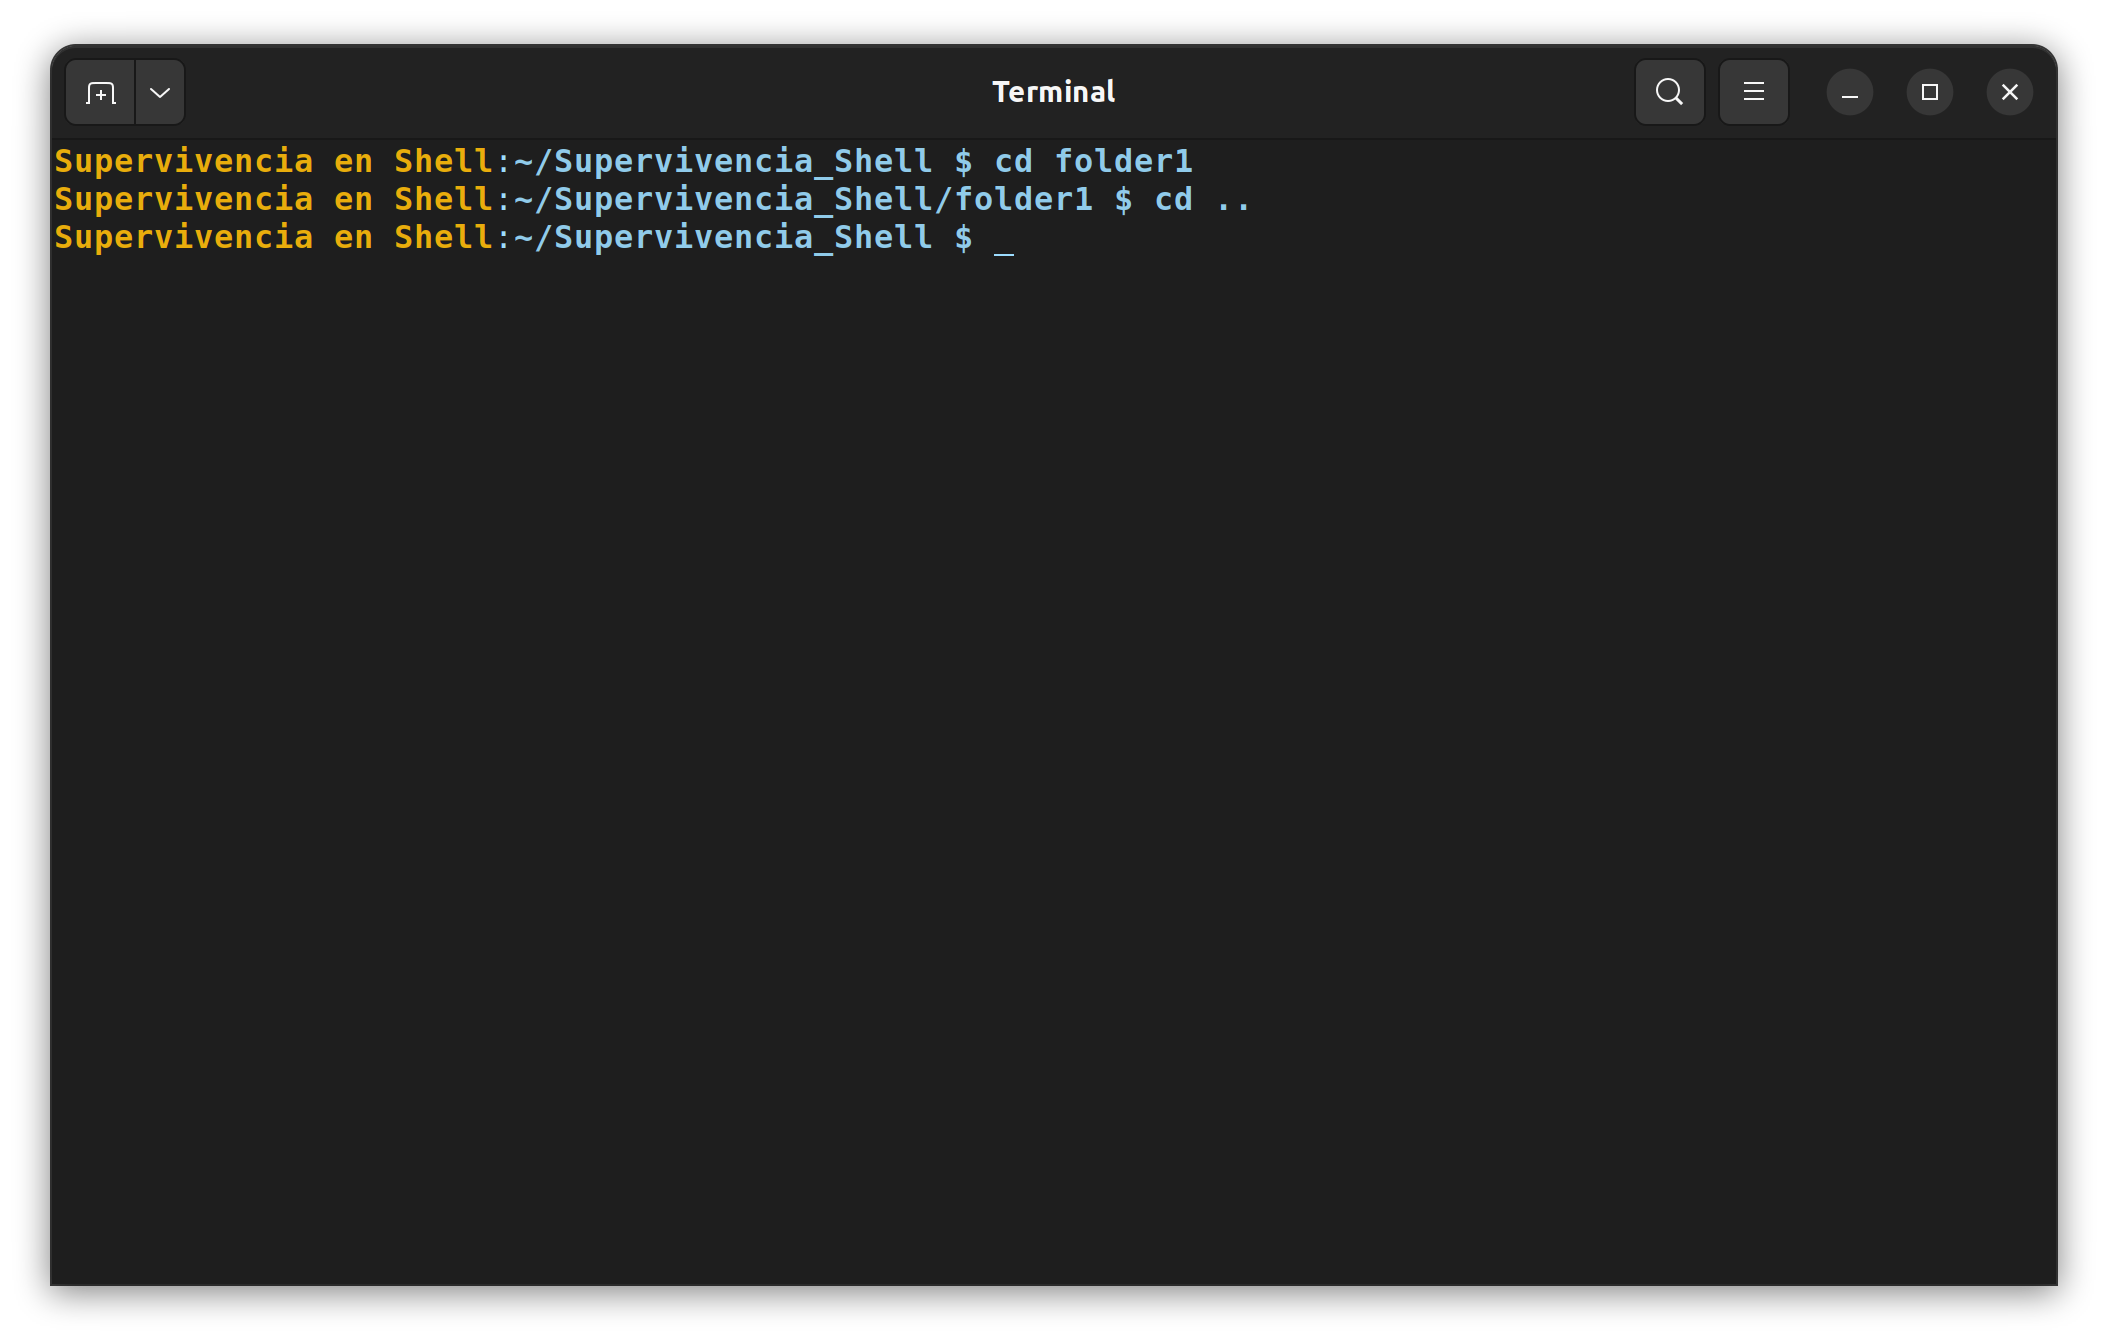
\includegraphics[width=0.75\textwidth]{cd}
	\end{frame}
	
	\begin{frame}
		\frametitle{Navegando por el terminal: touch}
		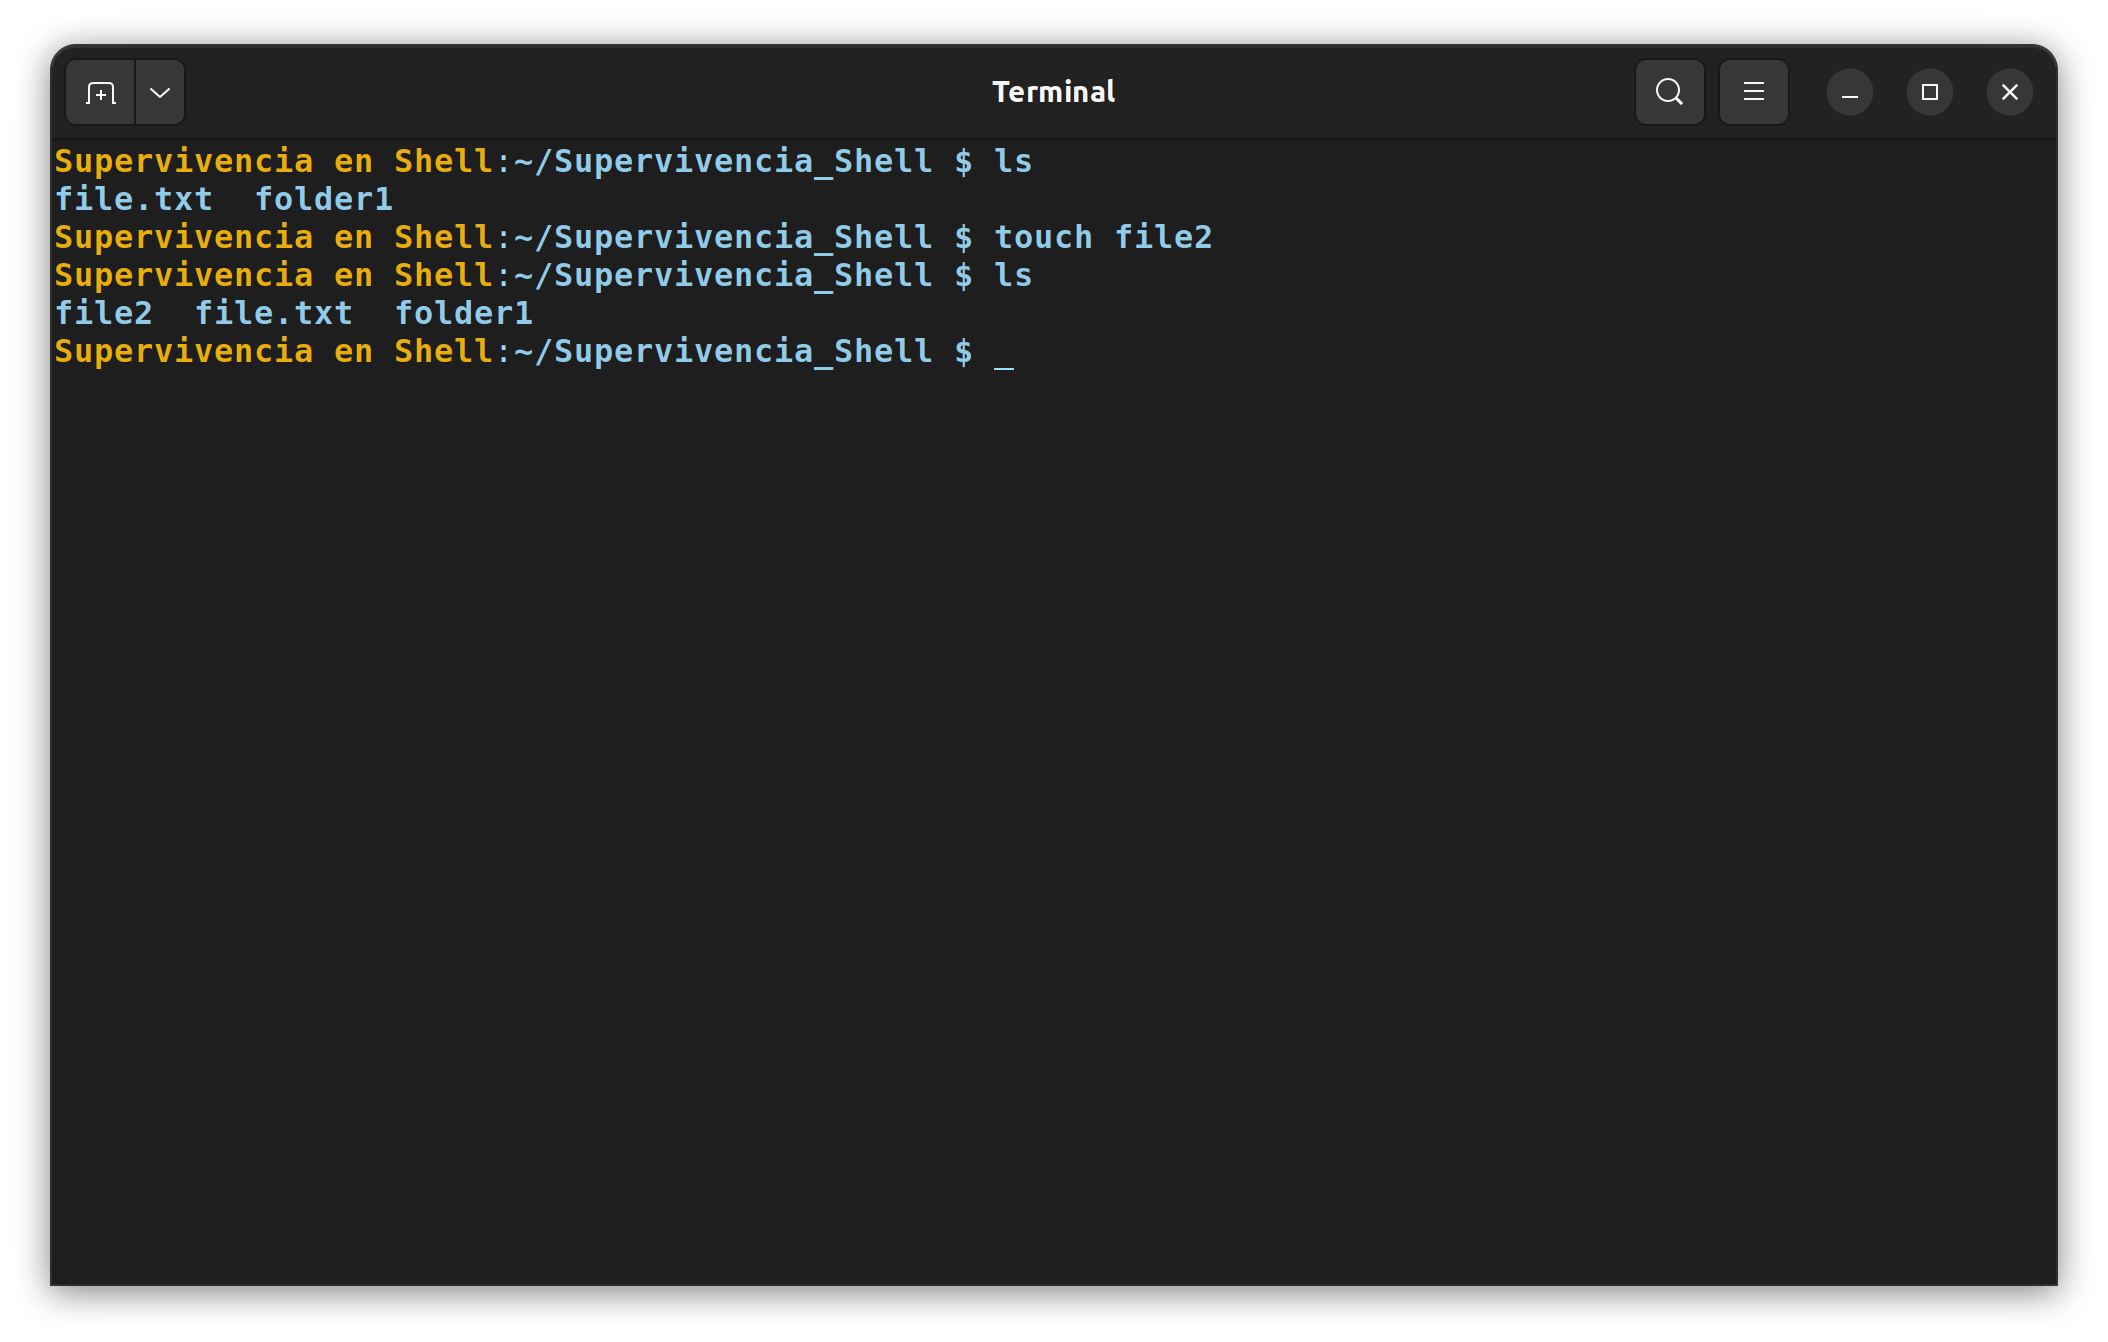
\includegraphics[width=0.75\textwidth]{touch}
	\end{frame}
	
	\begin{frame}
		\frametitle{Navegando por el terminal: cp}
		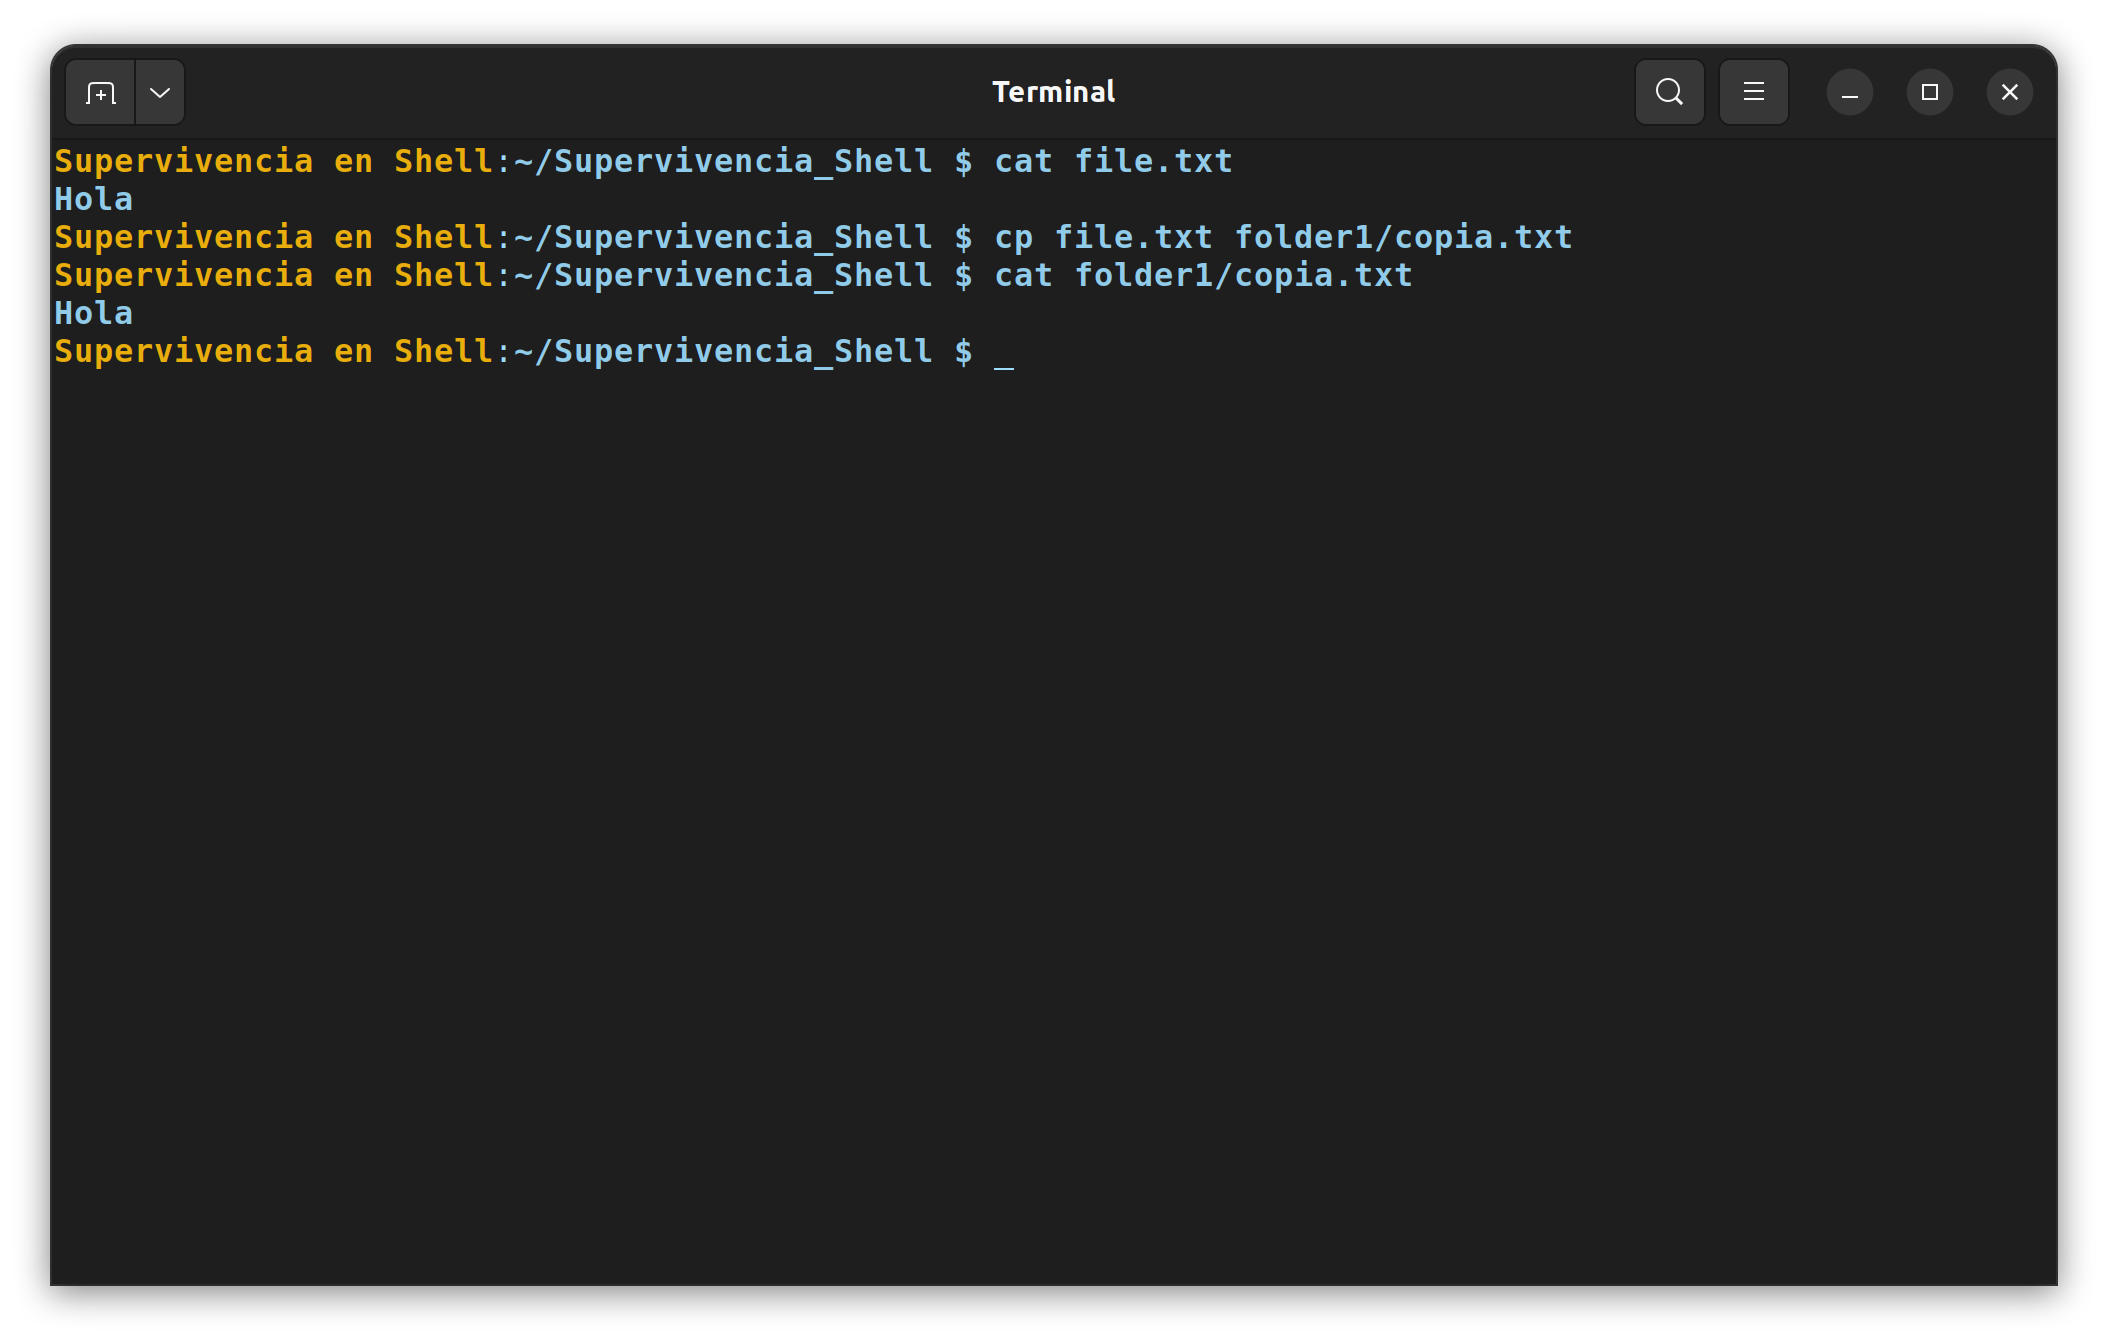
\includegraphics[width=0.75\textwidth]{cp}
	\end{frame}	
		
	\begin{frame}
		\frametitle{Navegando por el terminal: mv}
		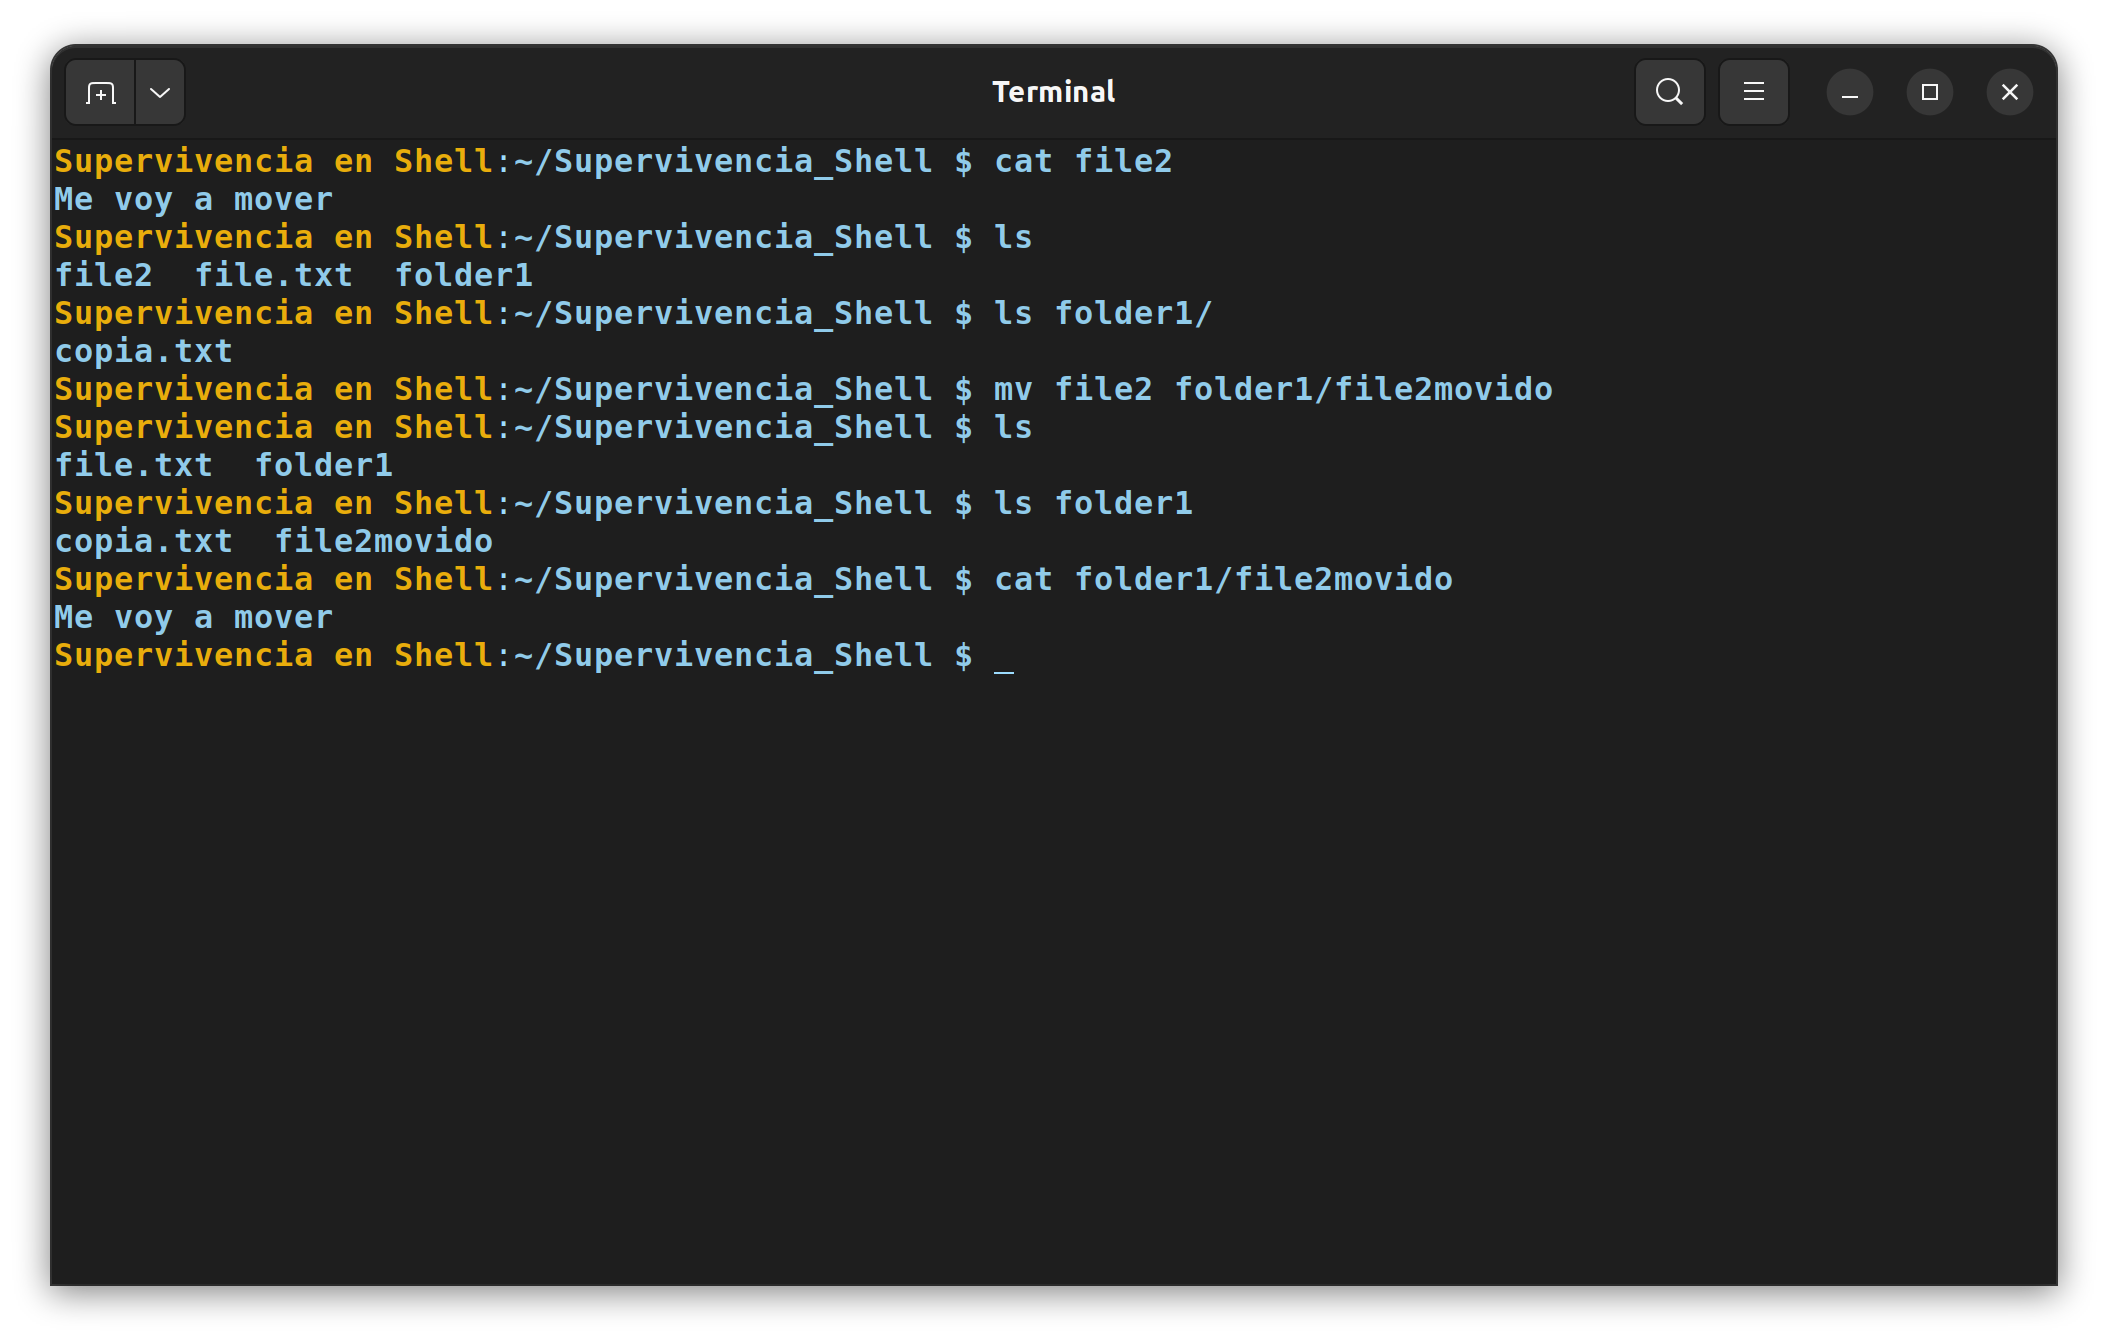
\includegraphics[width=0.75\textwidth]{mv}
	\end{frame}	
		
	\begin{frame}
		\frametitle{Navegando por el terminal: rm}
		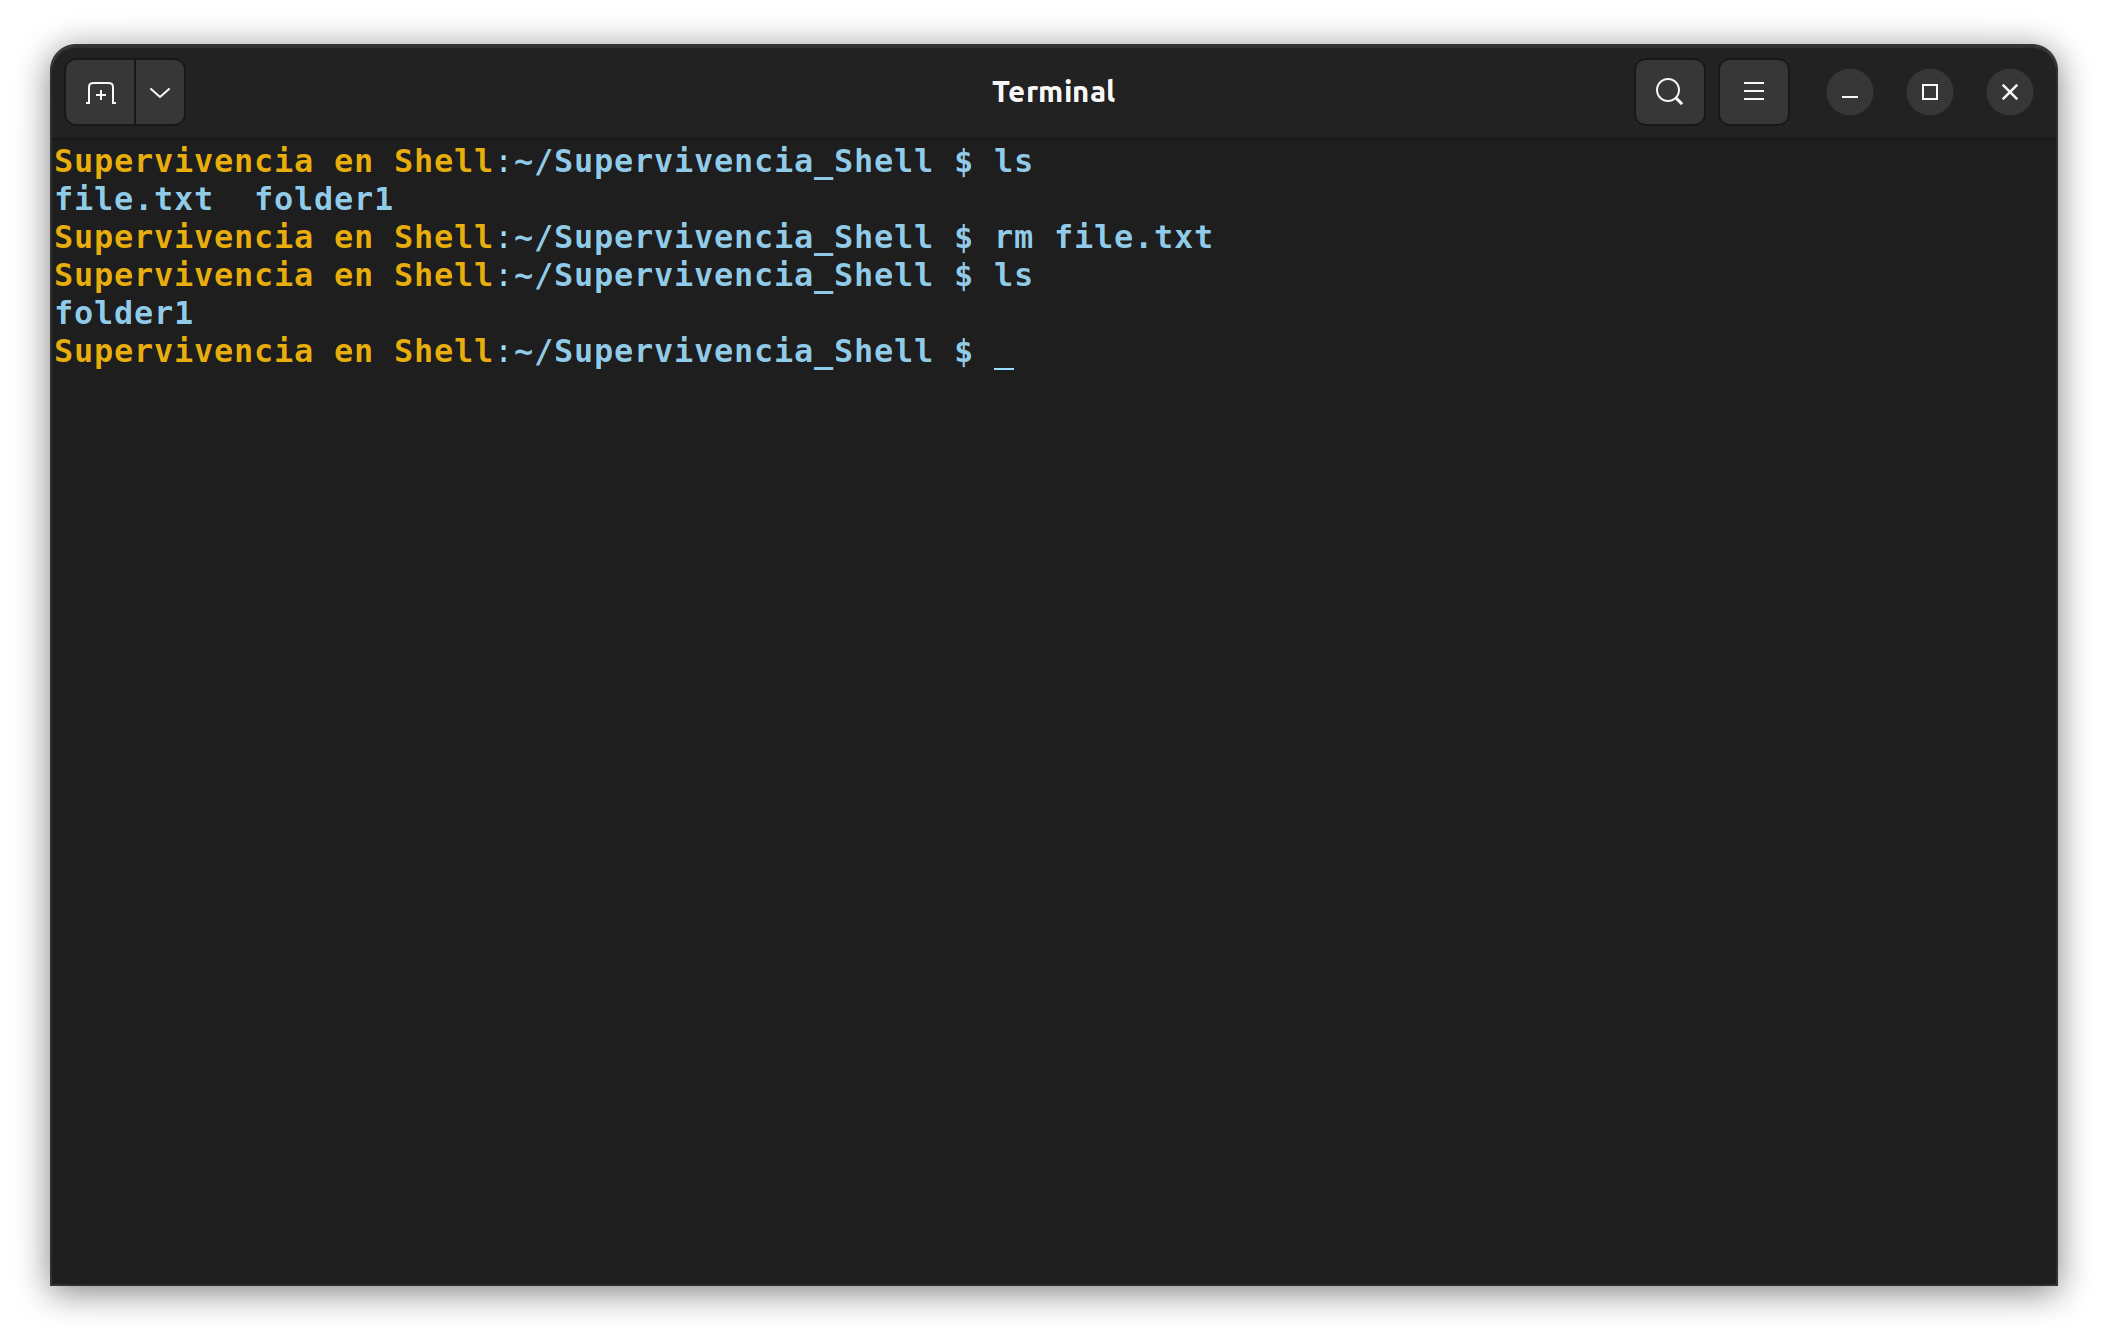
\includegraphics[width=0.75\textwidth]{rm}
	\end{frame}	
		
	\begin{frame}
		\frametitle{Navegando por el terminal: mkdir}
		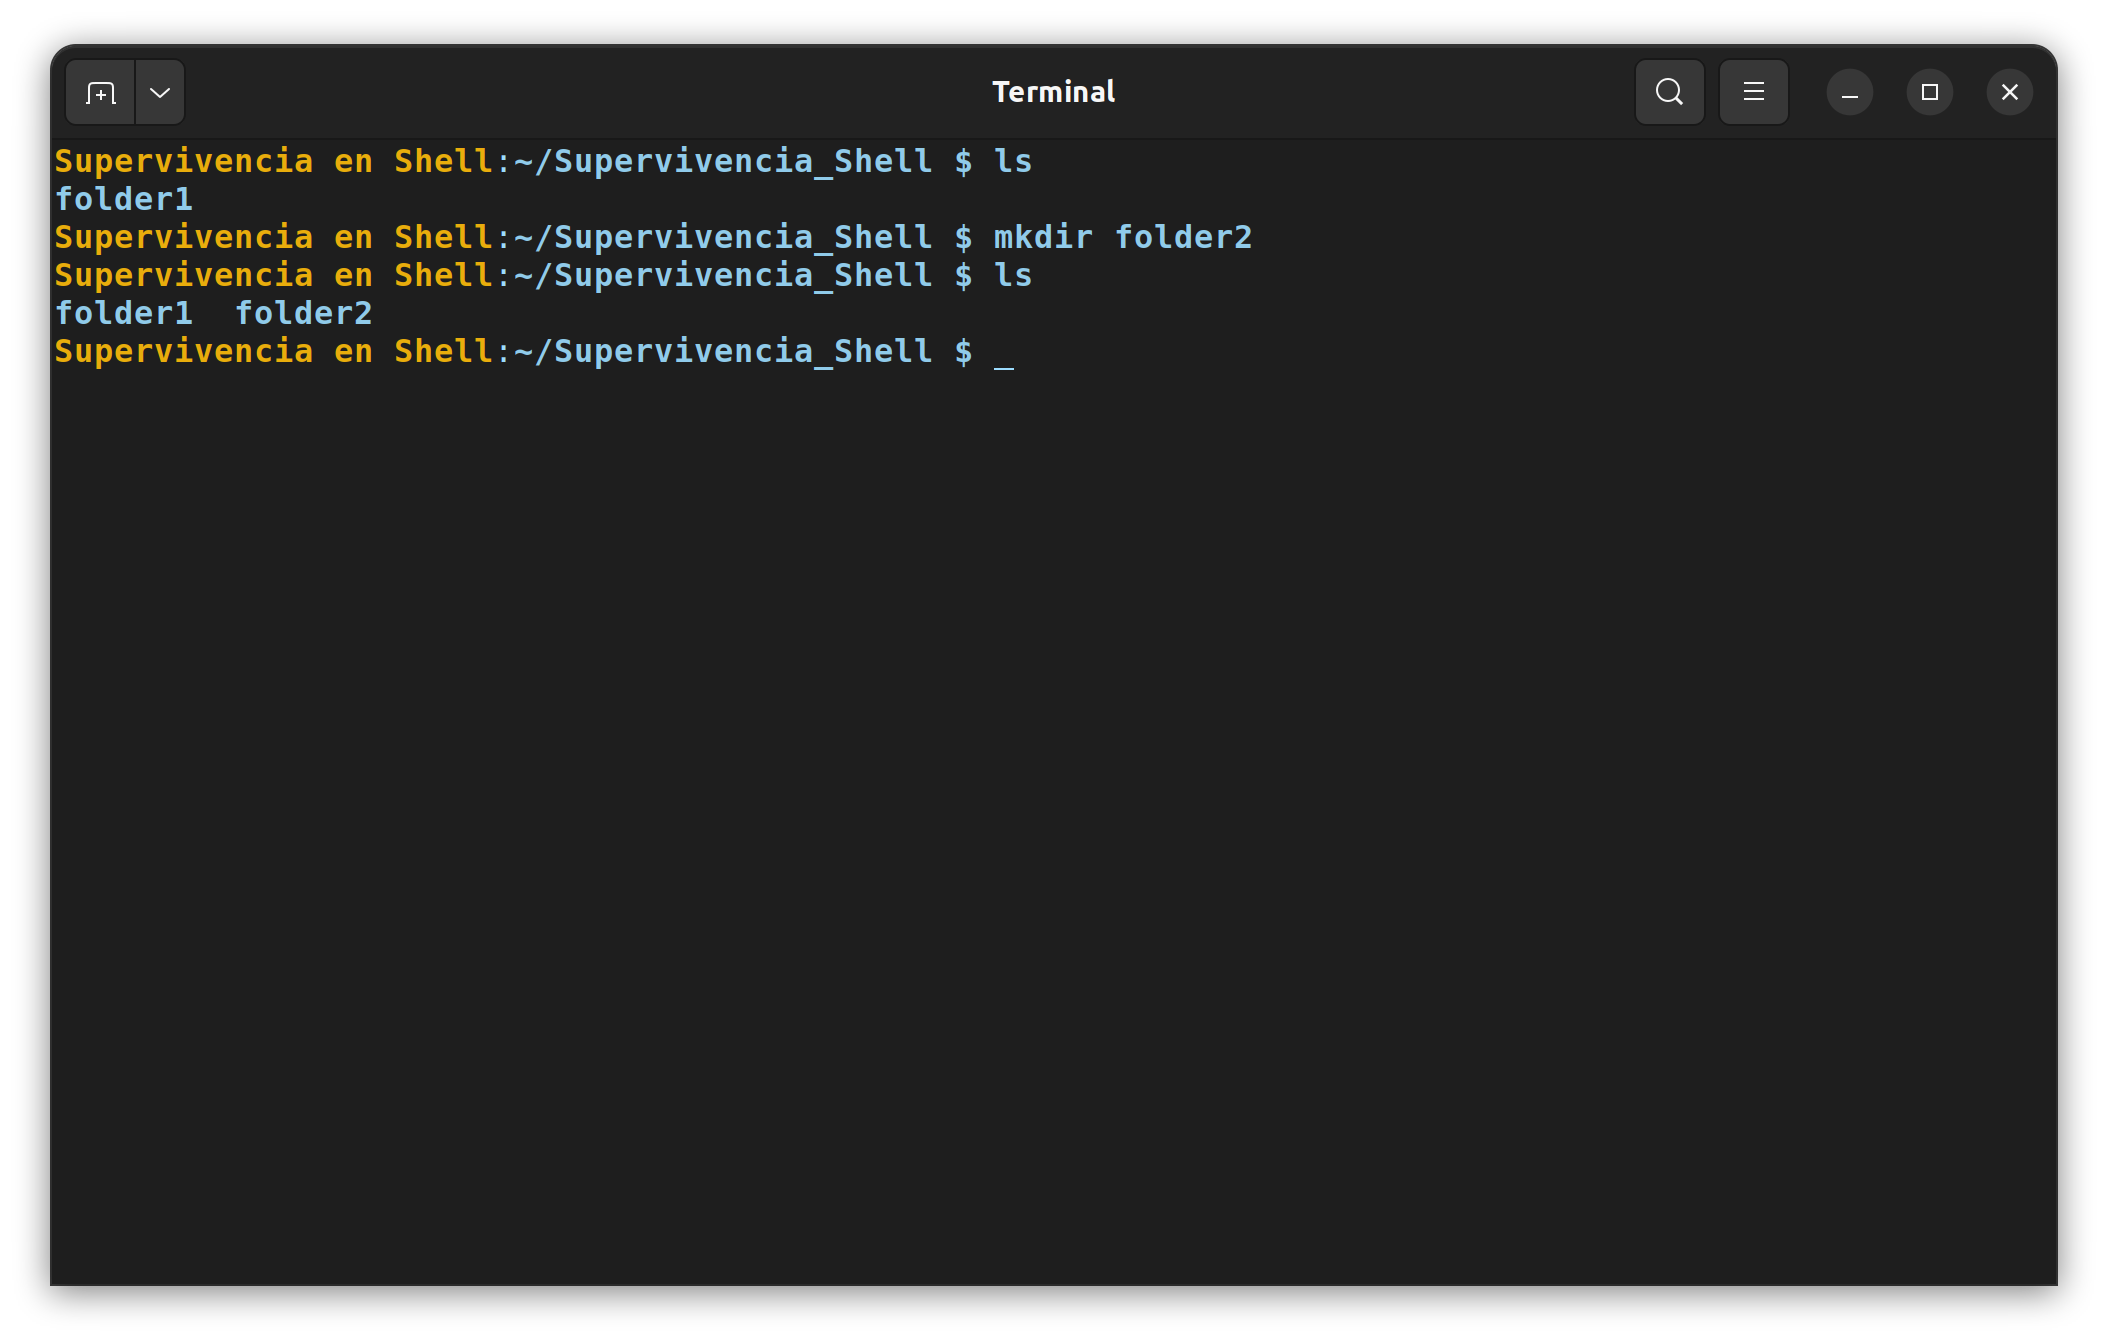
\includegraphics[width=0.75\textwidth]{mkdir}
	\end{frame}	

	\begin{frame}
		\frametitle{Navegando por el terminal: rmdir}
		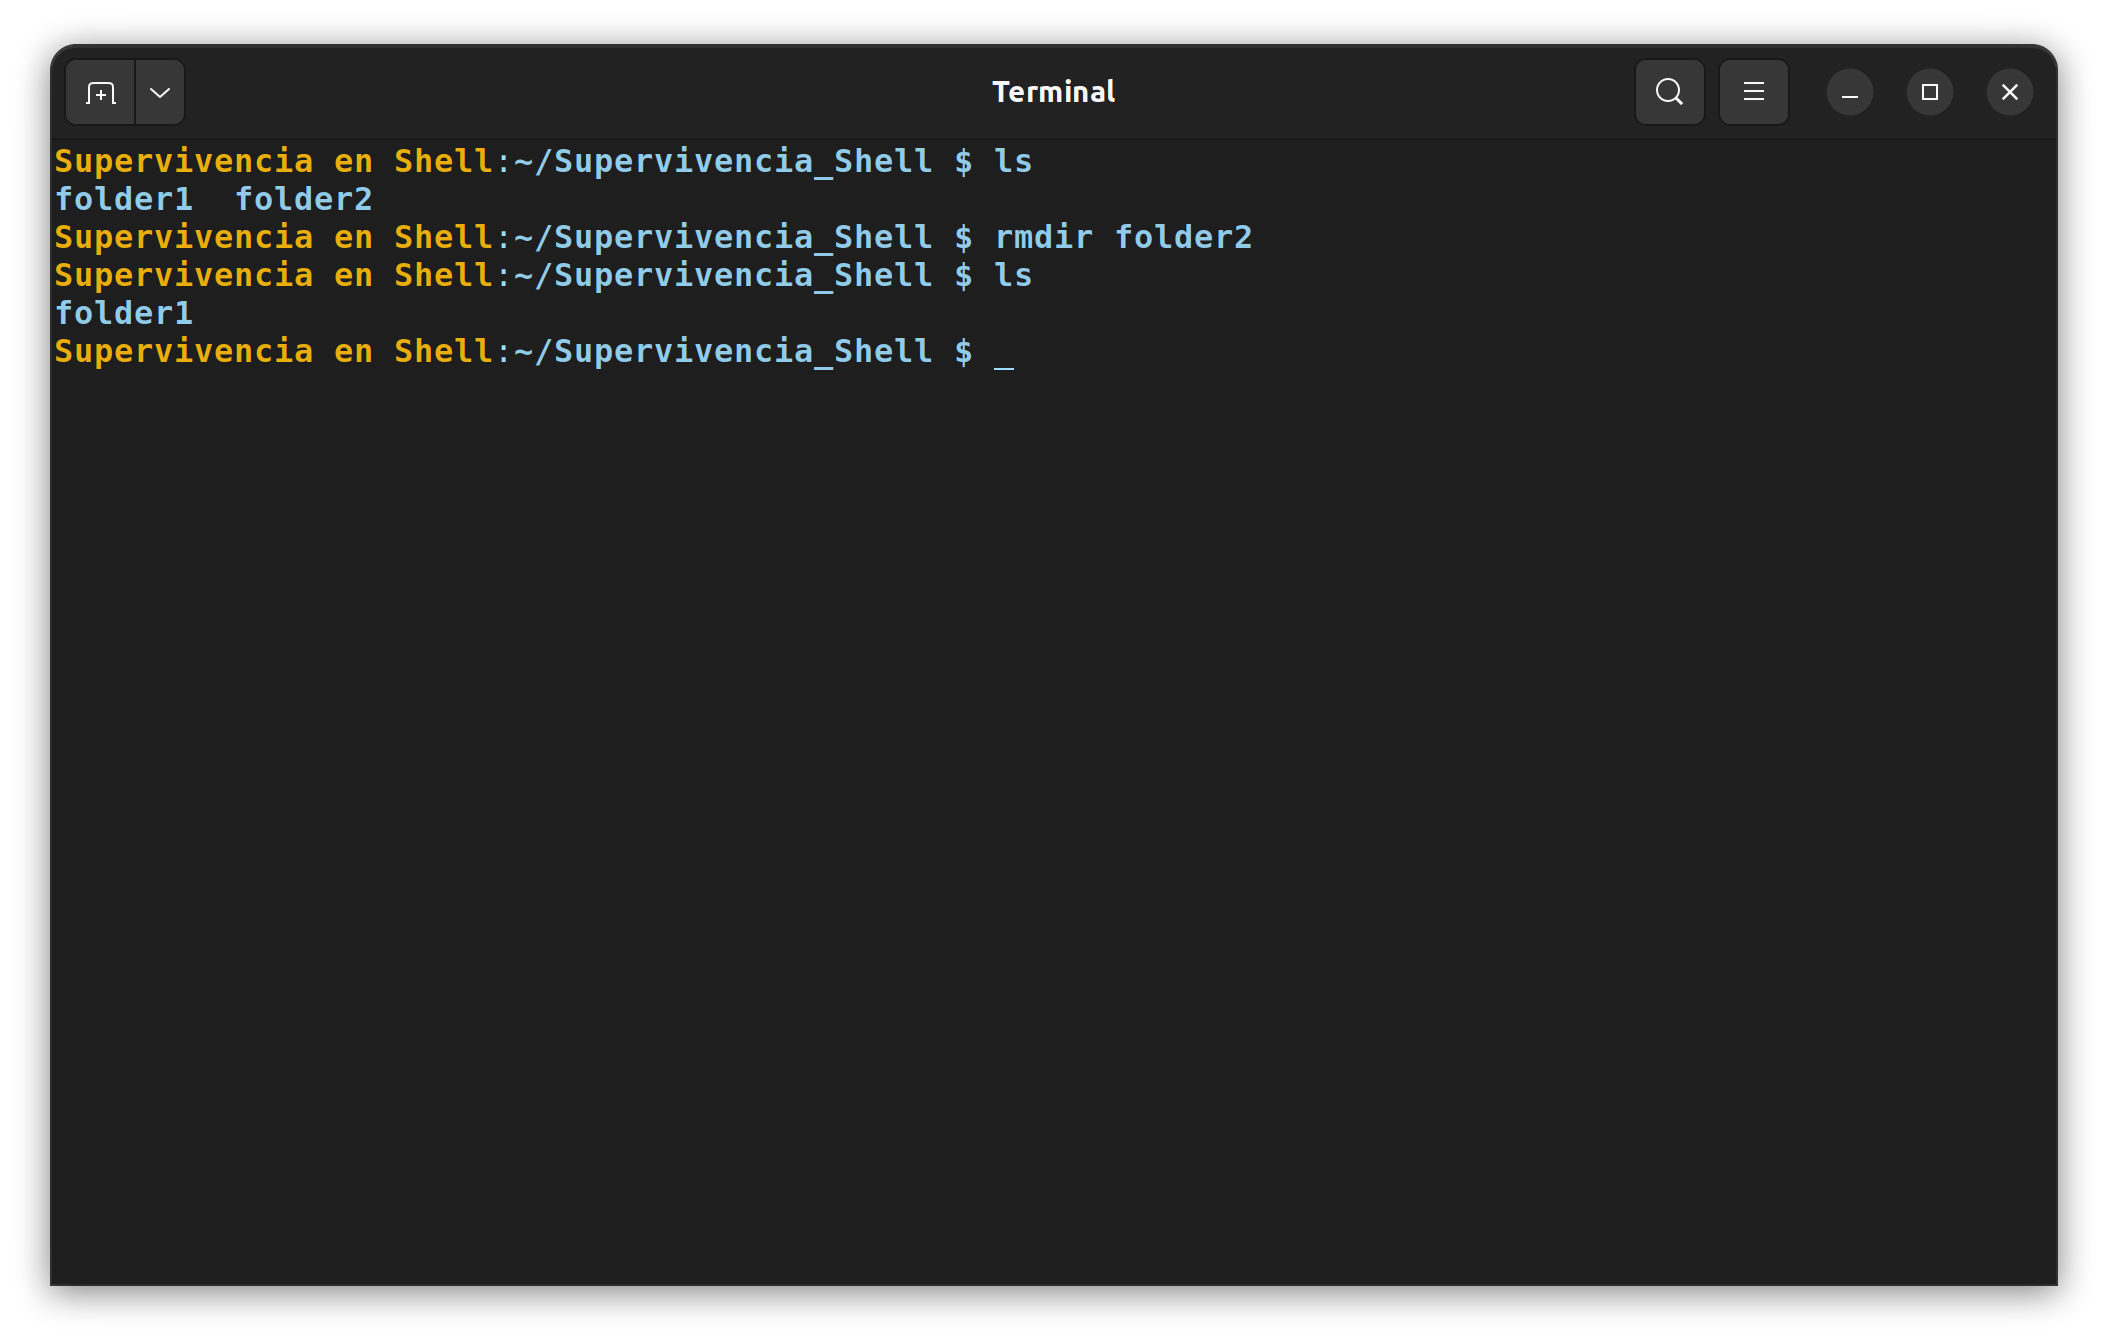
\includegraphics[width=0.75\textwidth]{rmdir}
	\end{frame}
	
	\begin{frame}
		\frametitle{Visualizando ficheros: cat}
		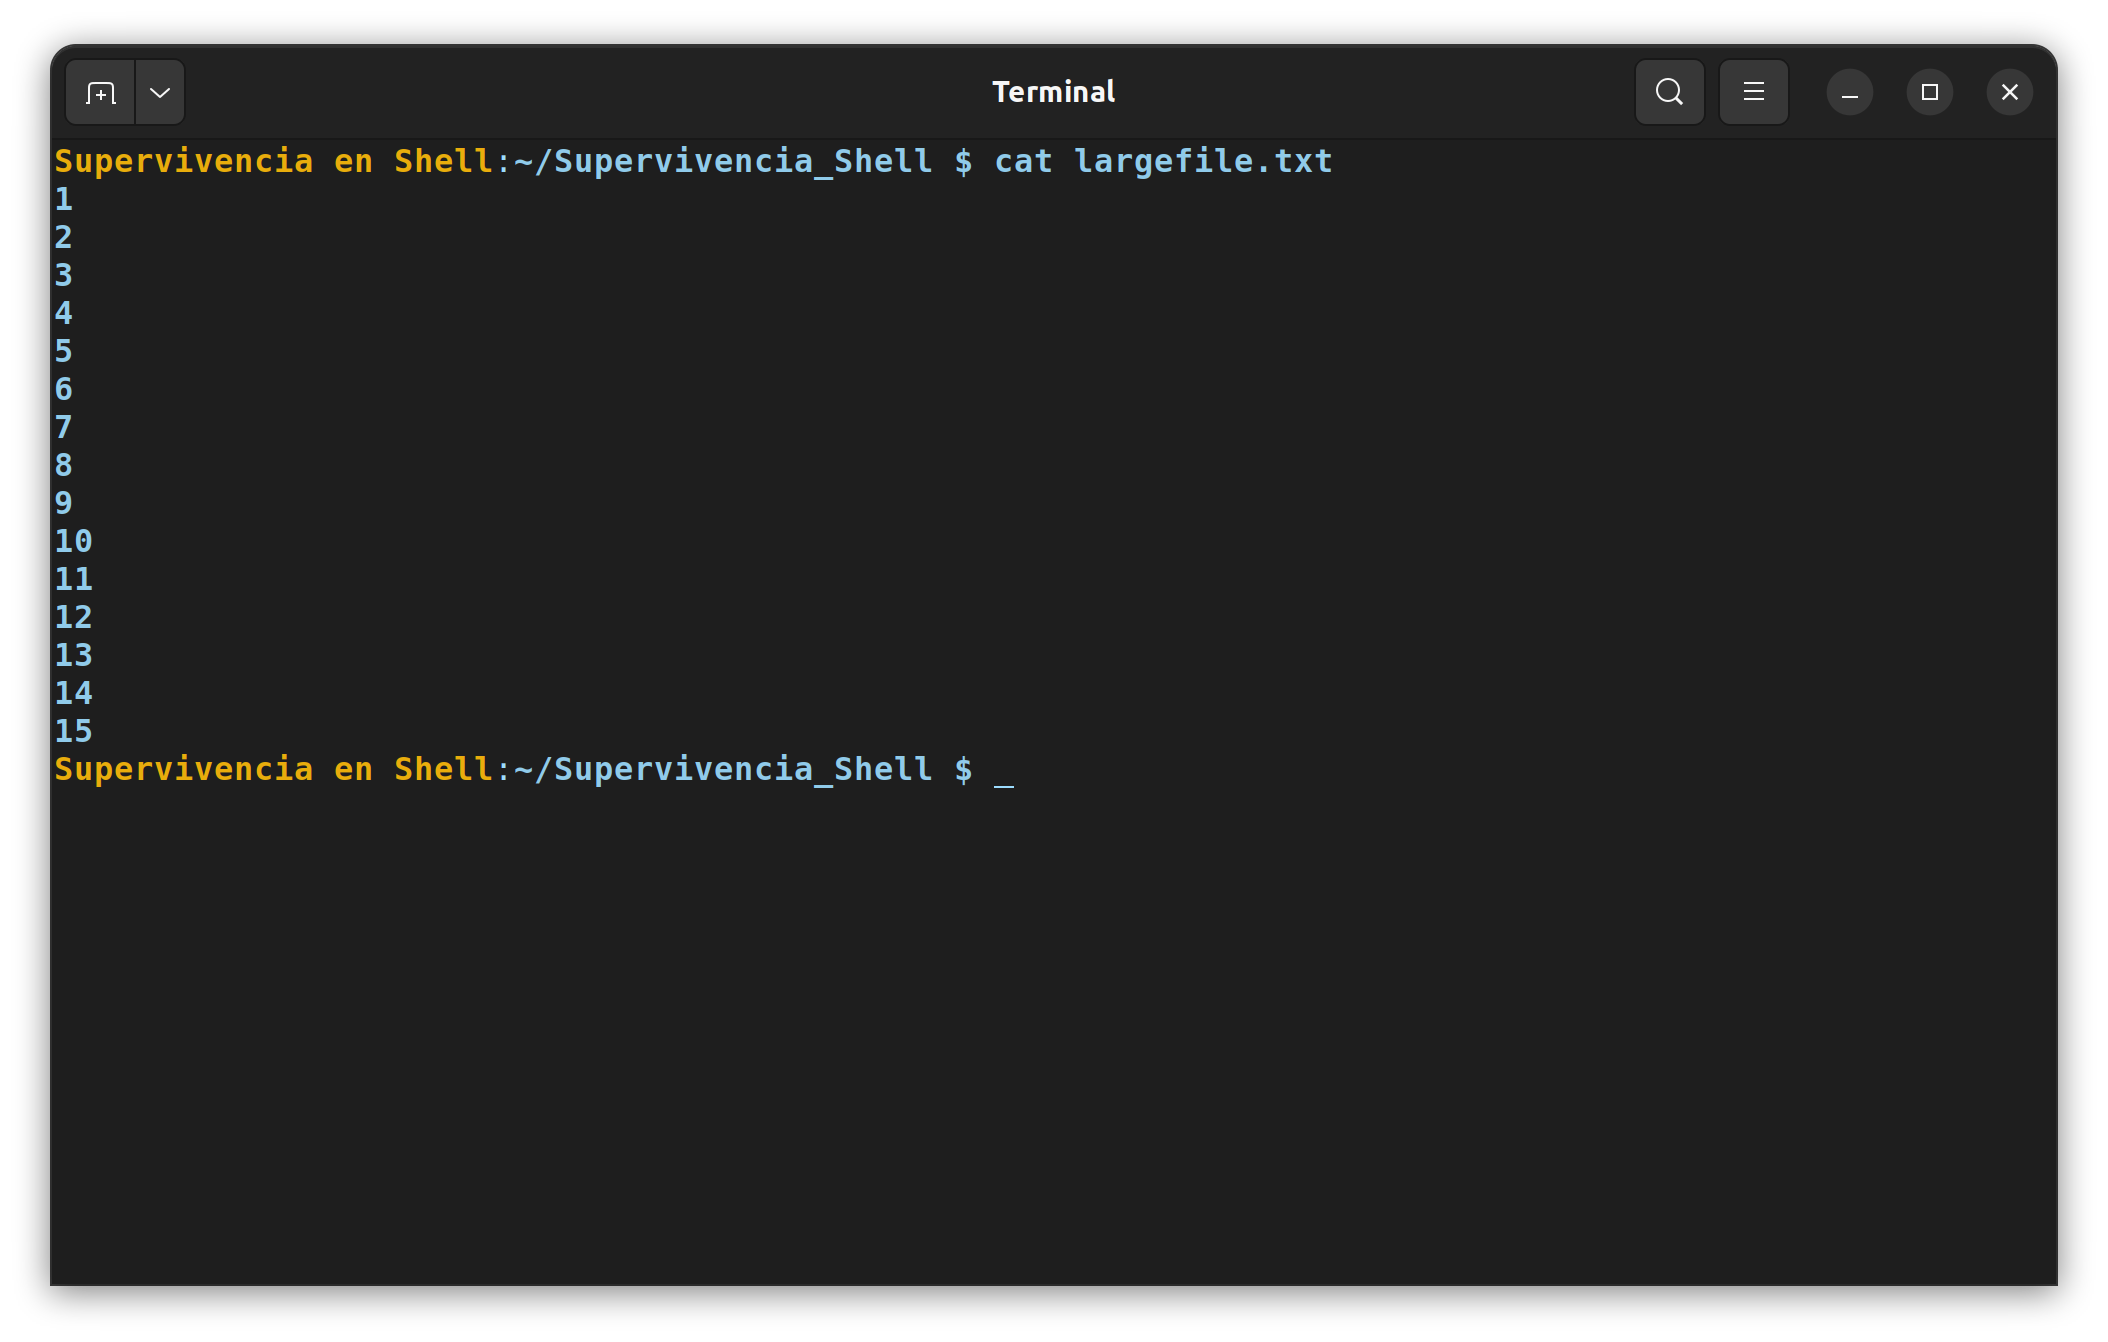
\includegraphics[width=0.75\textwidth]{cat}
	\end{frame}	
	
	\begin{frame}
		\frametitle{Visualizando ficheros: less}
		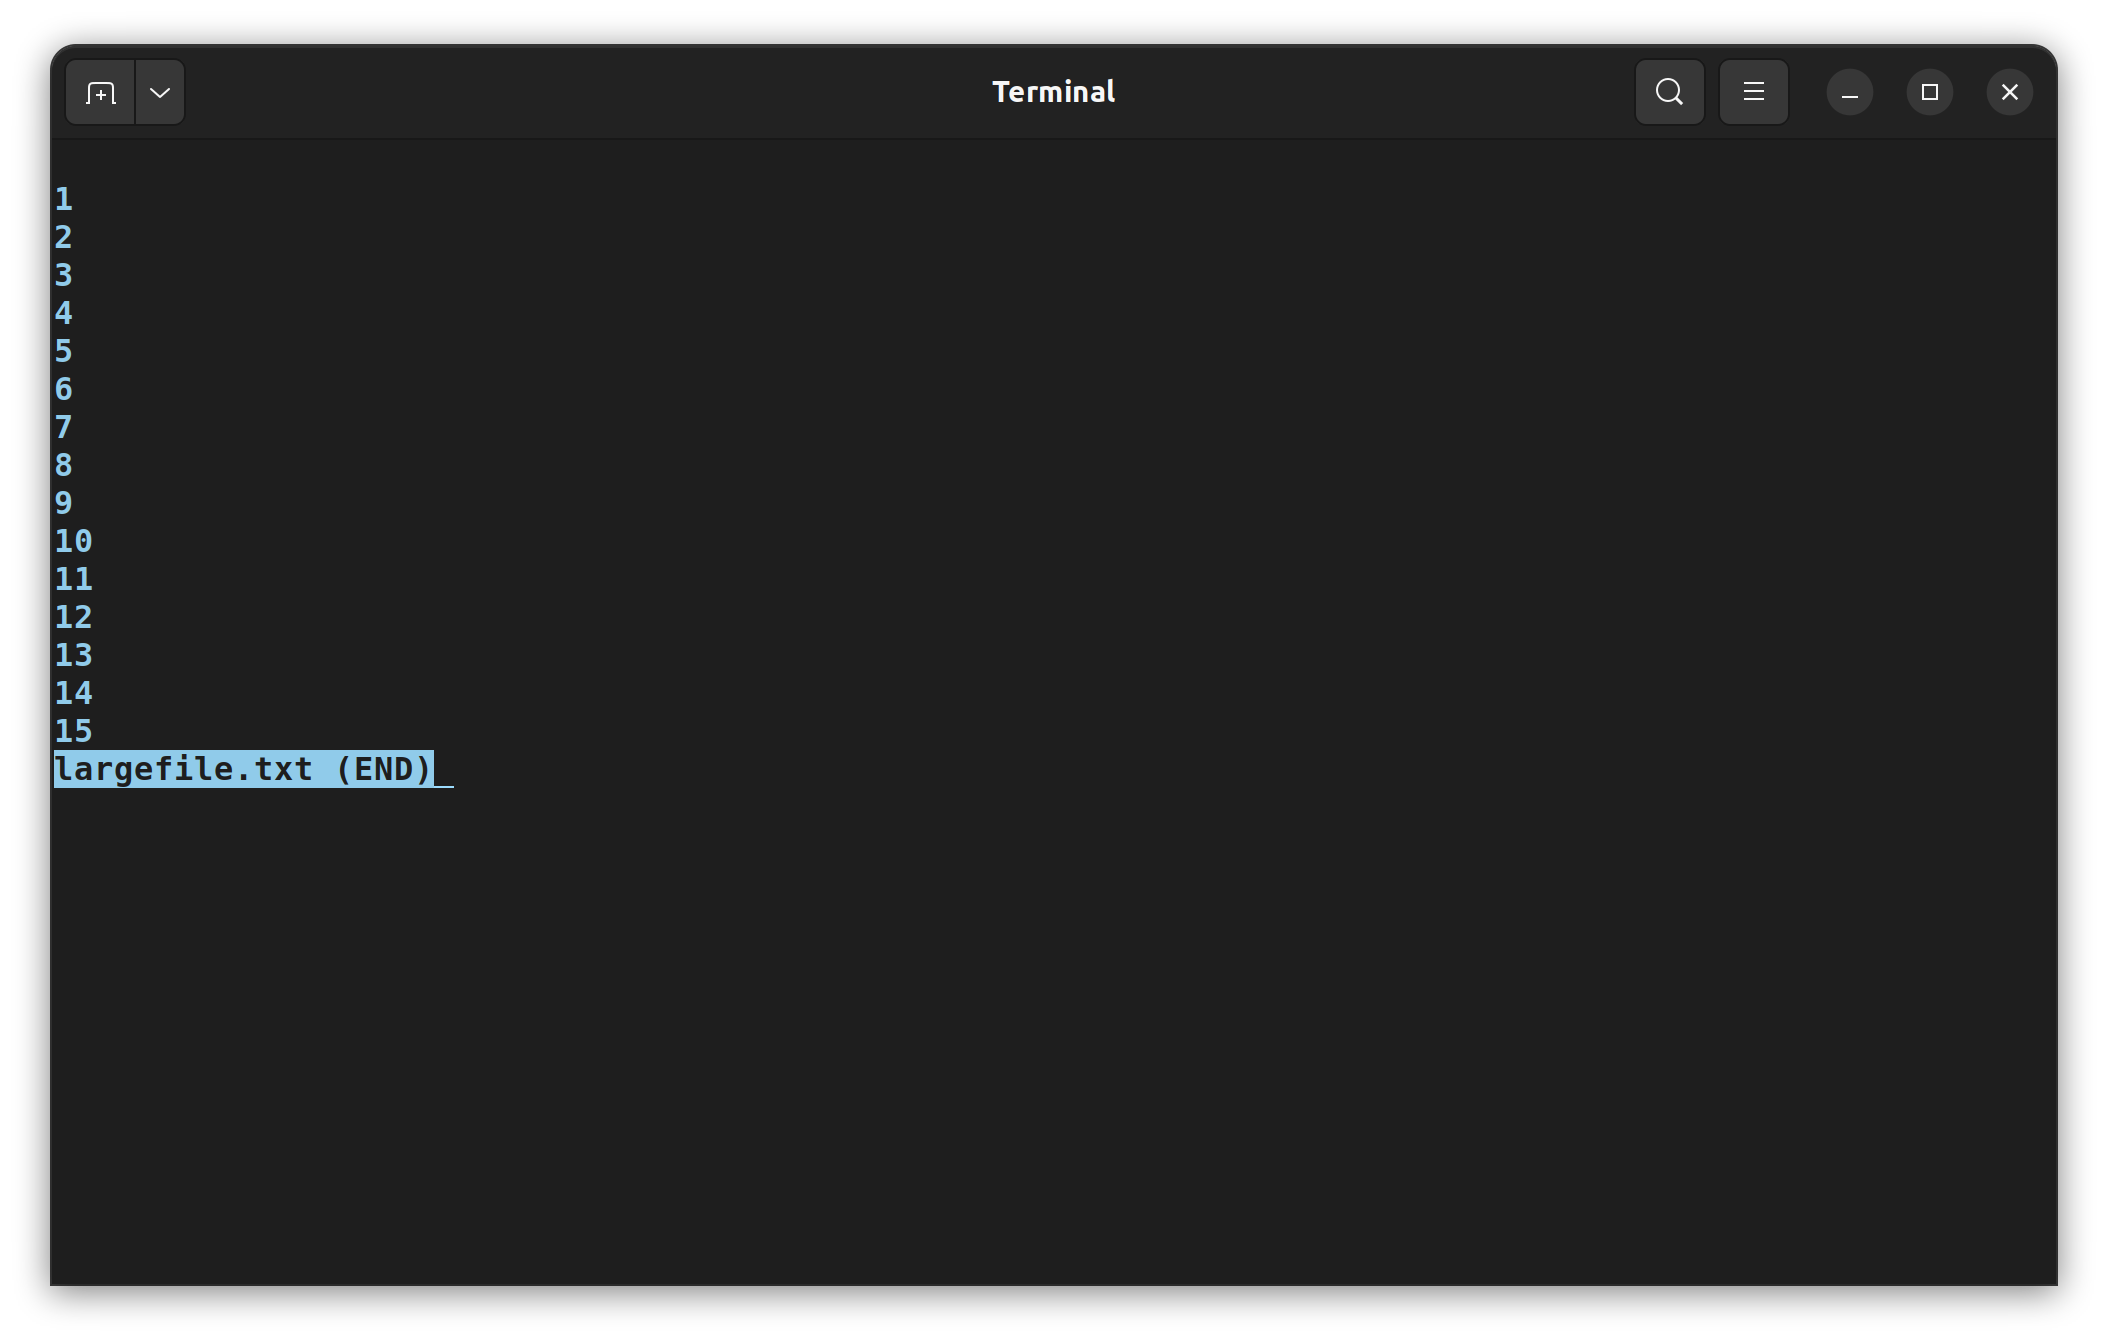
\includegraphics[width=0.75\textwidth]{less}
	\end{frame}
		
	\begin{frame}
		\frametitle{Visualizando ficheros: head}
		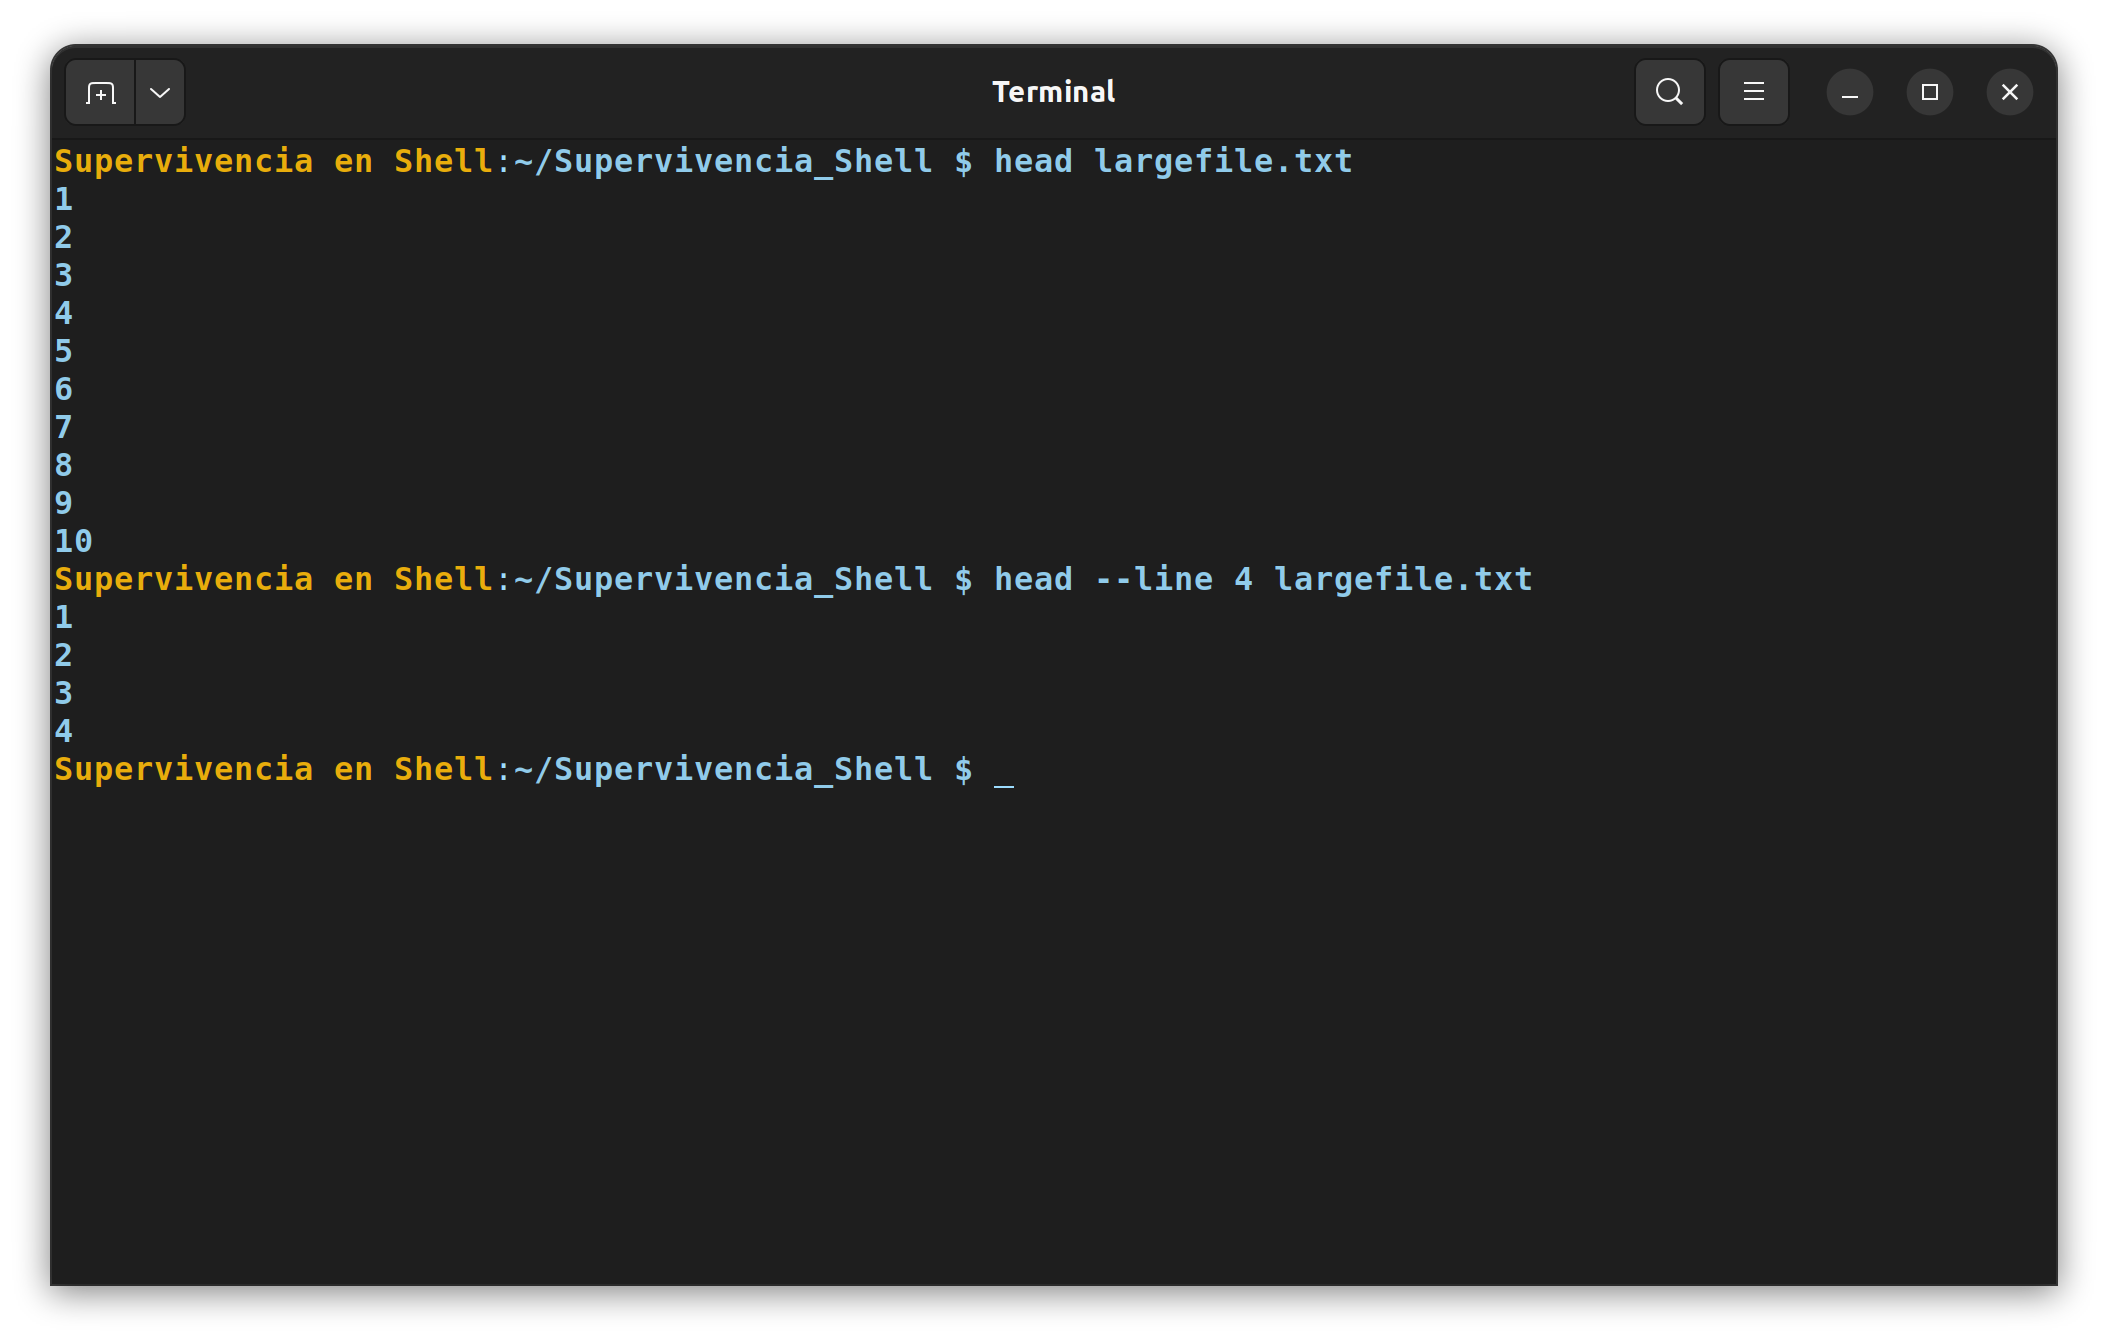
\includegraphics[width=0.75\textwidth]{head}
	\end{frame}	
	
	\begin{frame}
		\frametitle{Visualizando ficheros: tail}
		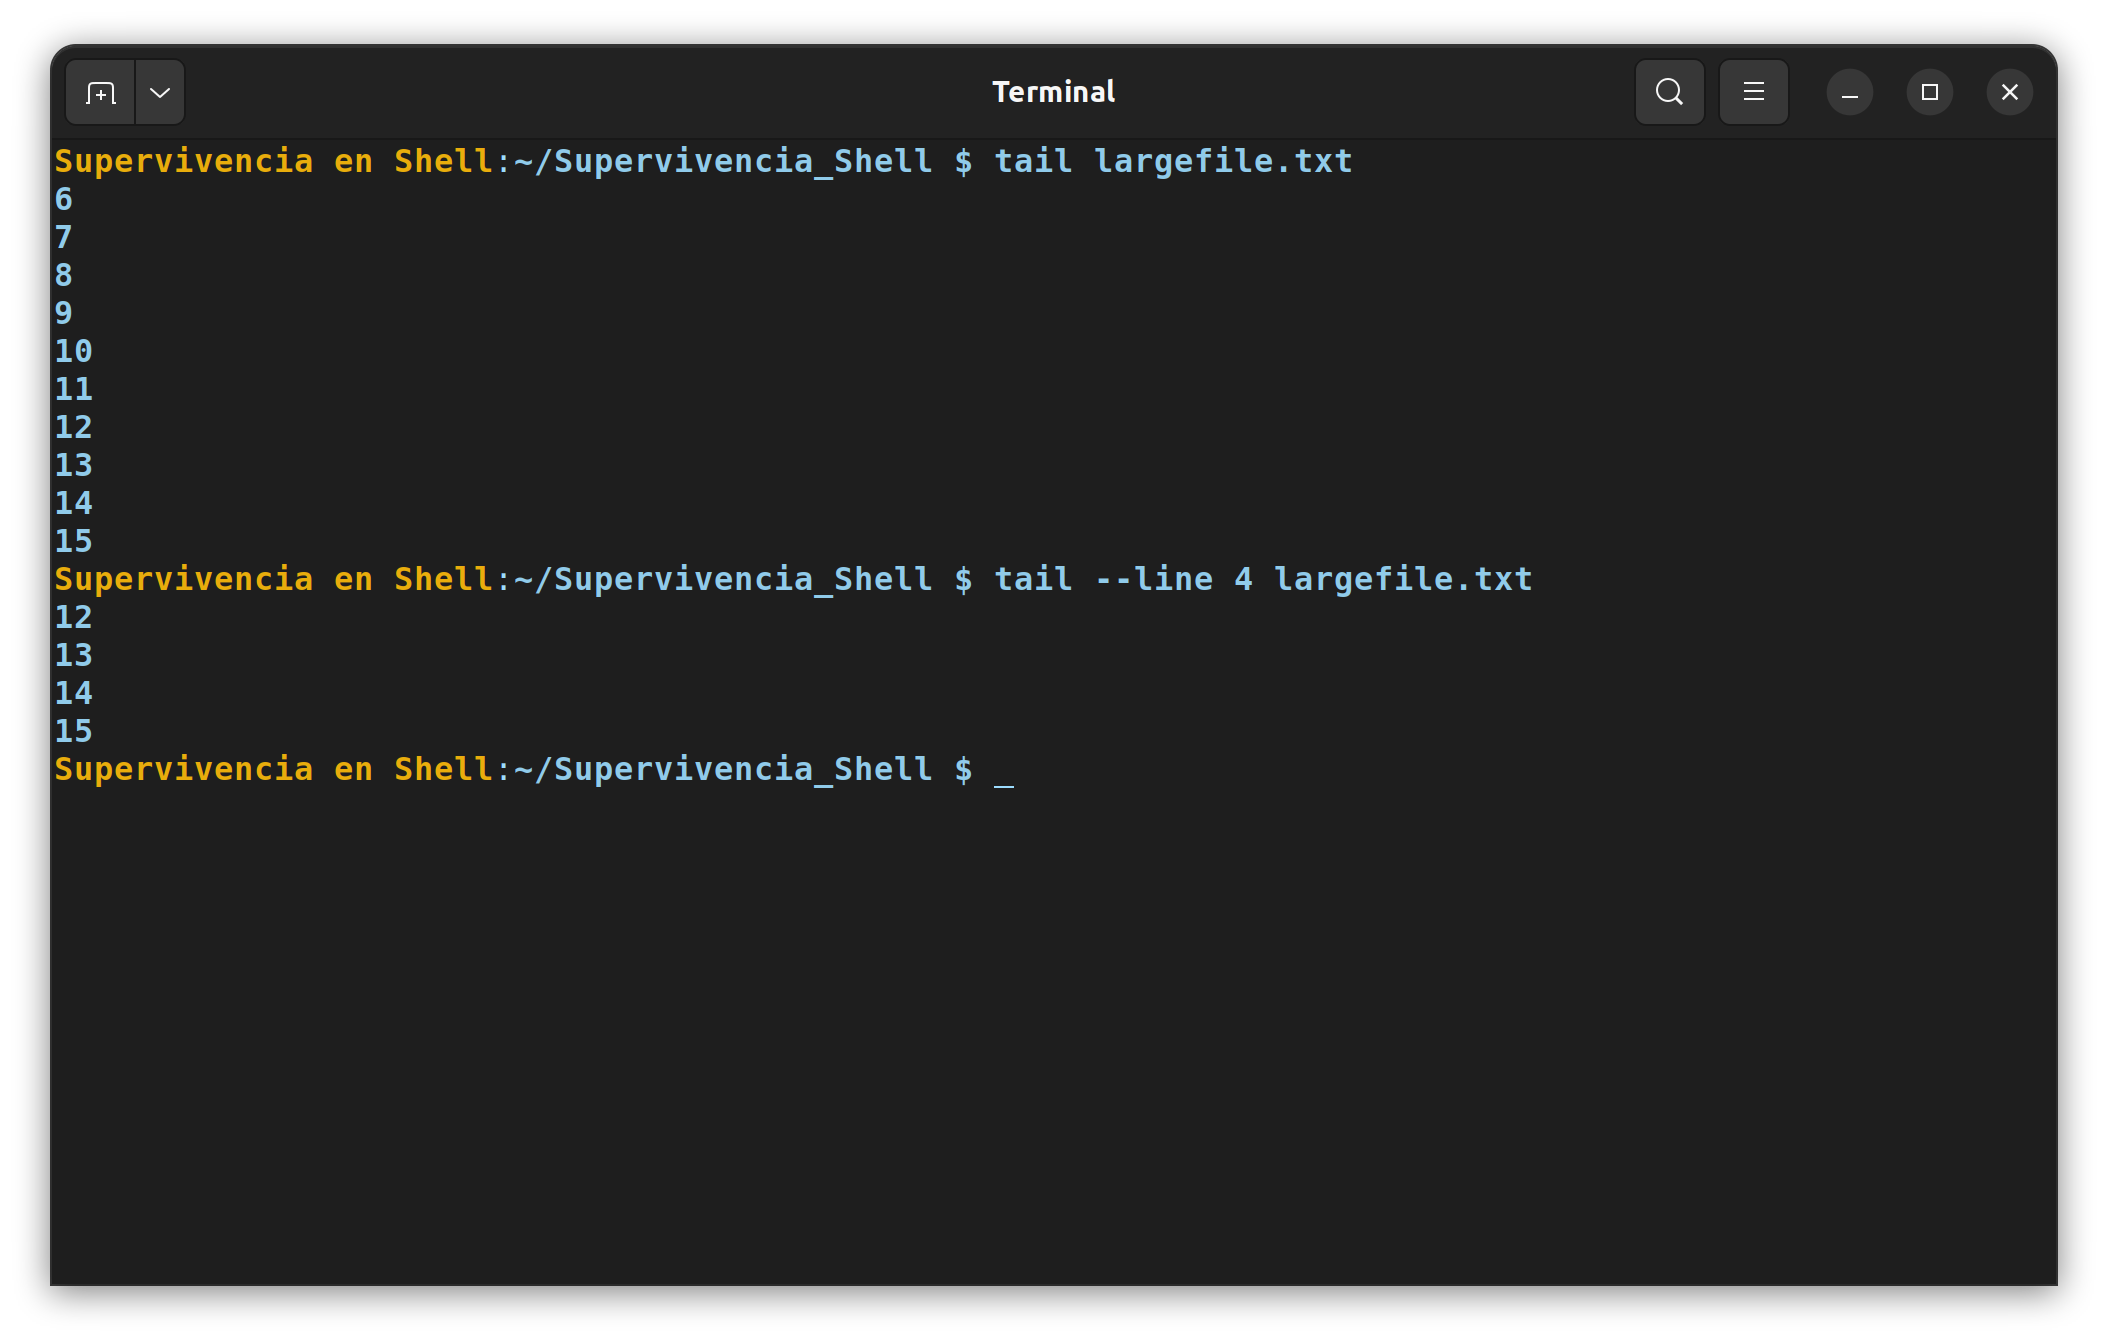
\includegraphics[width=0.75\textwidth]{tail}
	\end{frame}
		
	\begin{frame}
		\frametitle{Visualizando ficheros: file}
		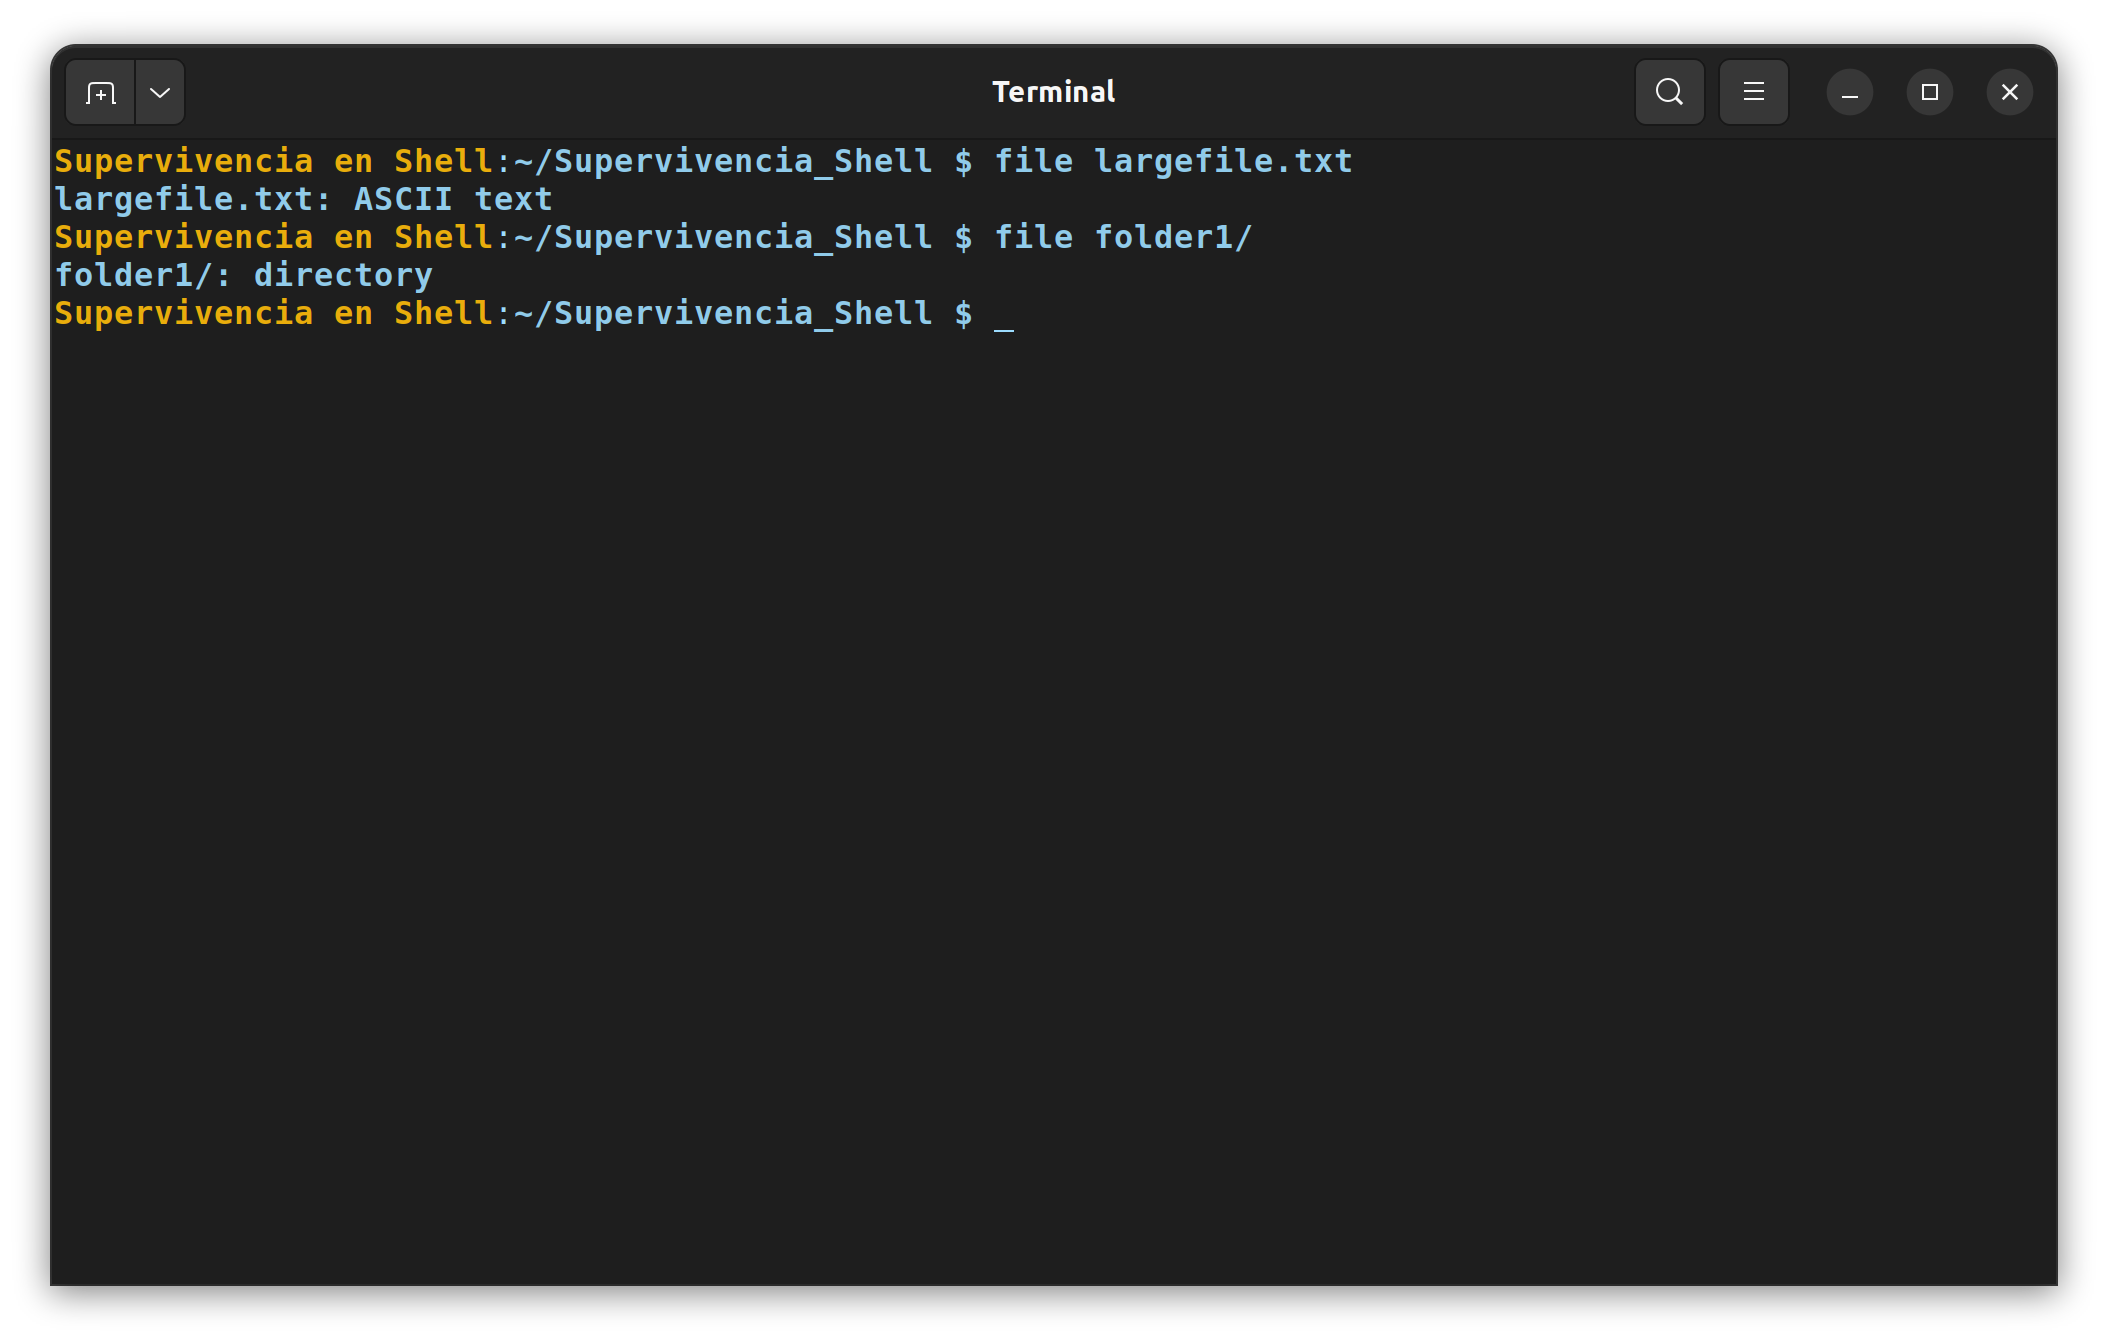
\includegraphics[width=0.75\textwidth]{file}
	\end{frame}
		
	\begin{frame}
		\frametitle{Buscando en ficheros: grep/fgrep}
		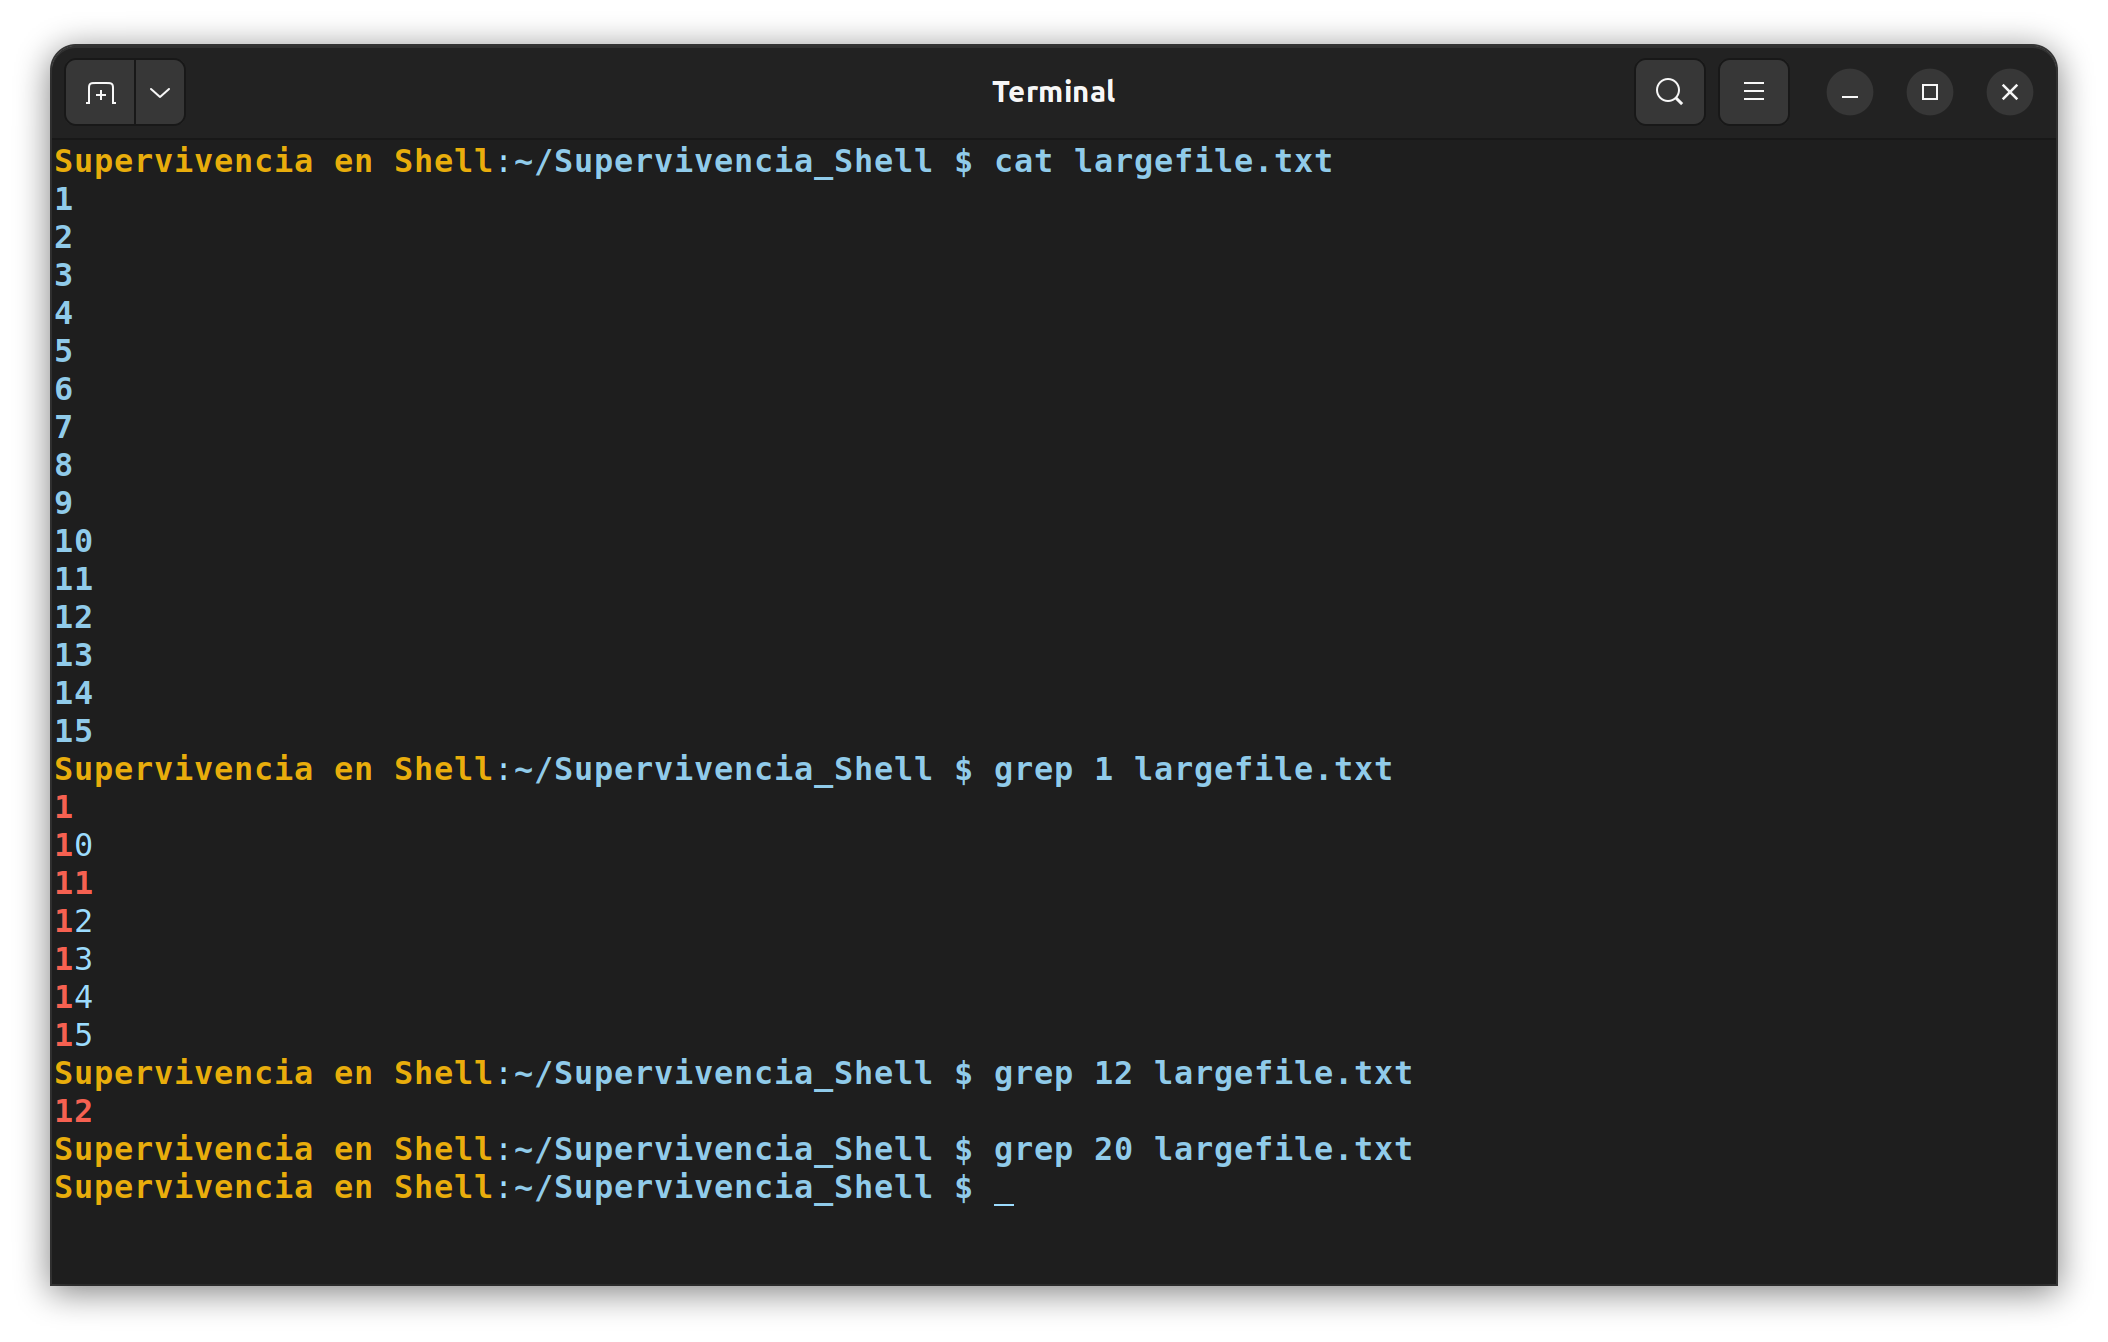
\includegraphics[width=0.75\textwidth]{grep}
	\end{frame}
	
	\begin{frame}
		\frametitle{Ordenando ficheros: sort}
		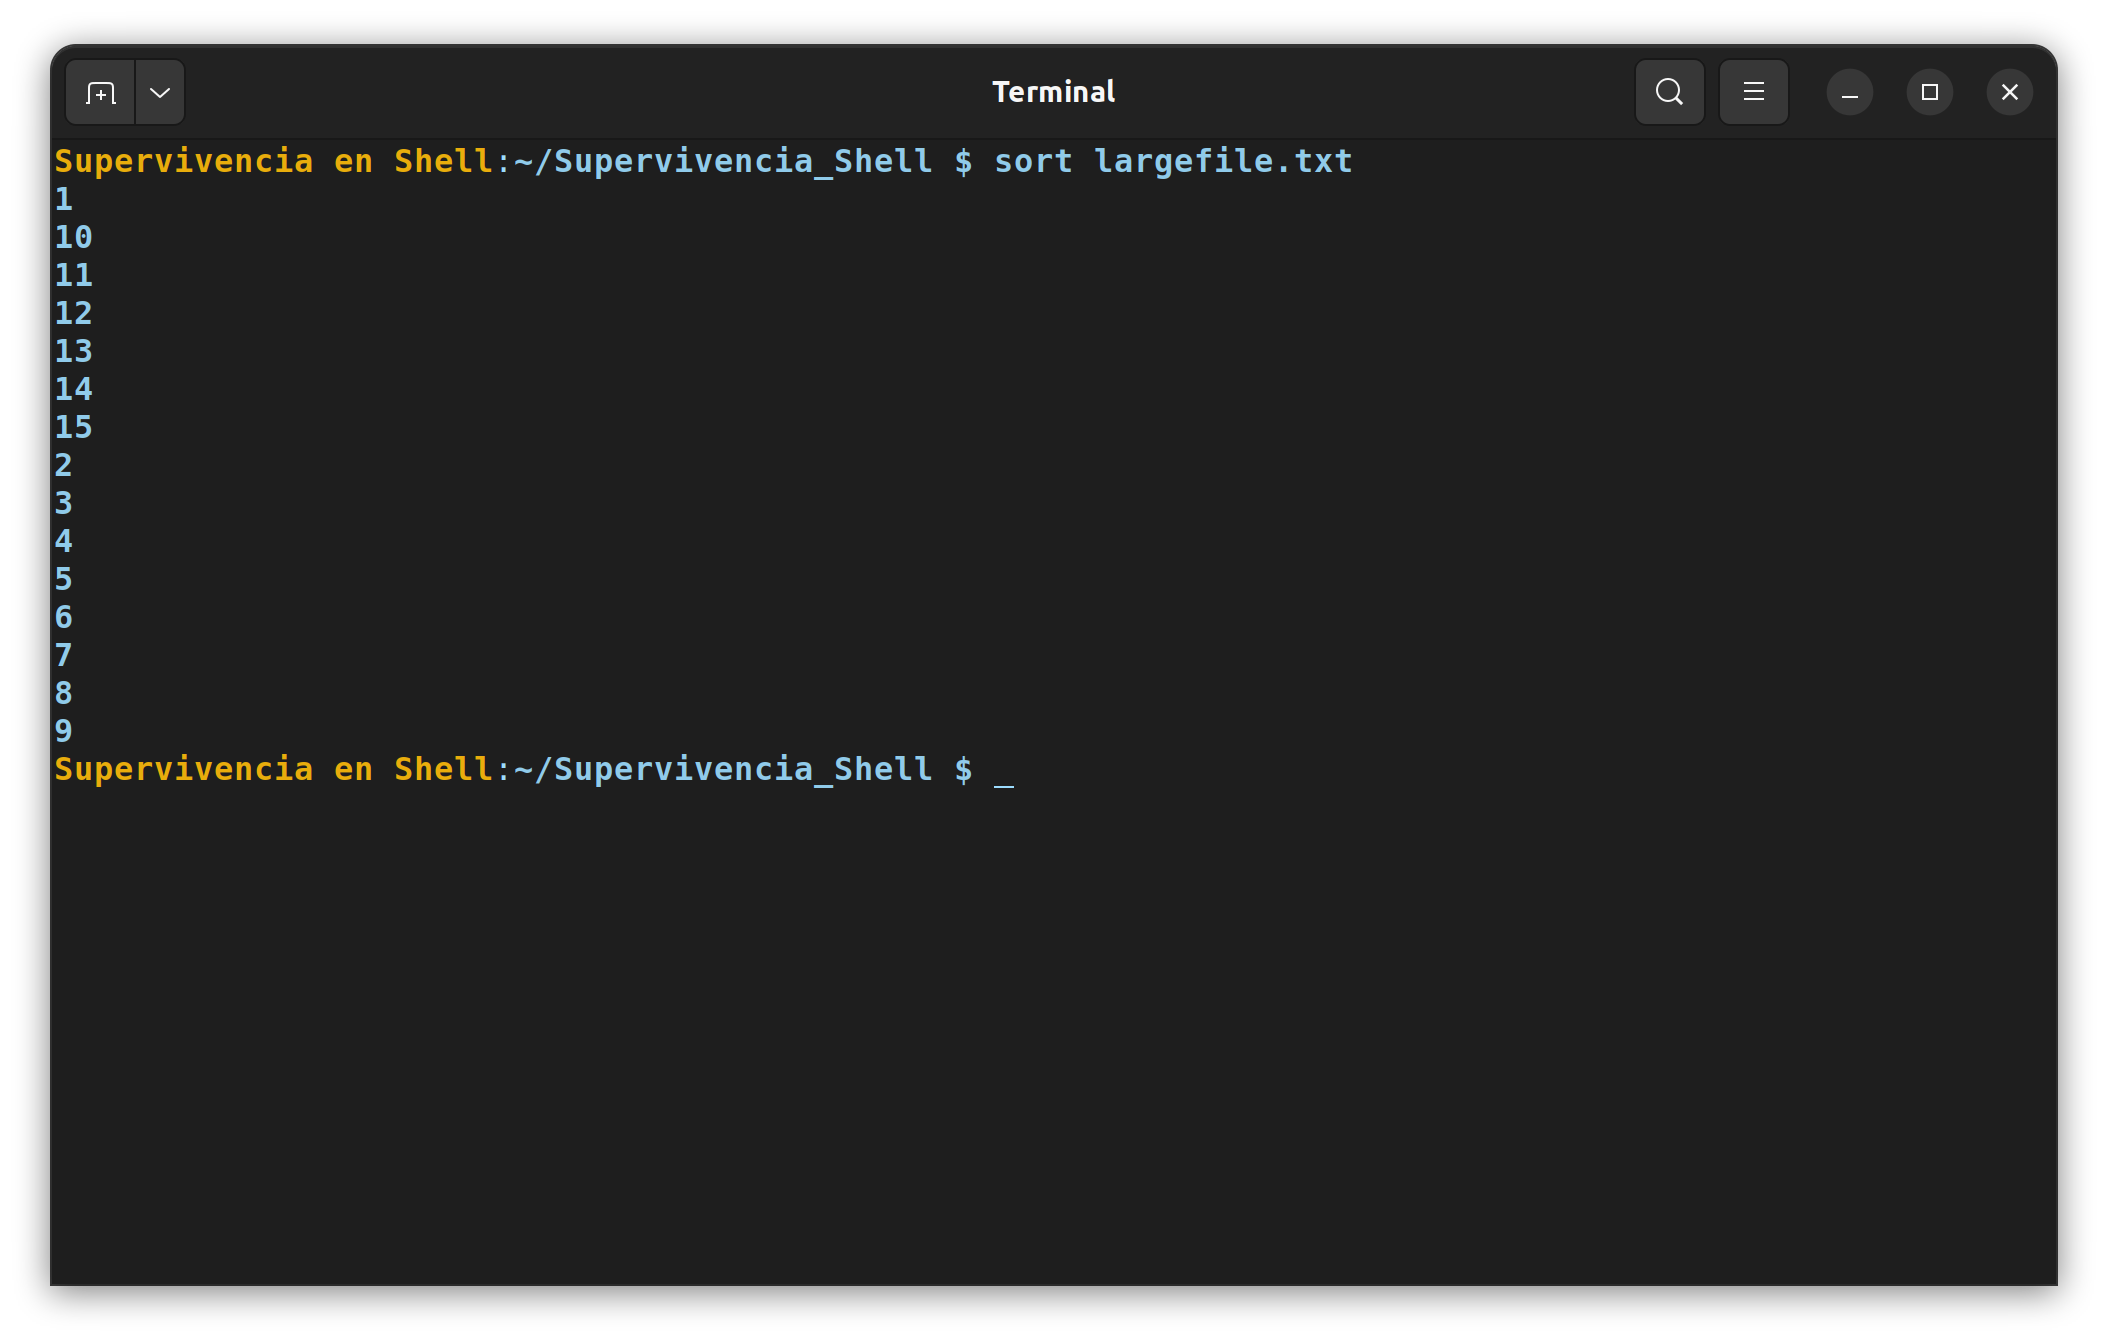
\includegraphics[width=0.75\textwidth]{sort}
	\end{frame}
		
	\begin{frame}
		\frametitle{Comparando ficheros: cmp}
		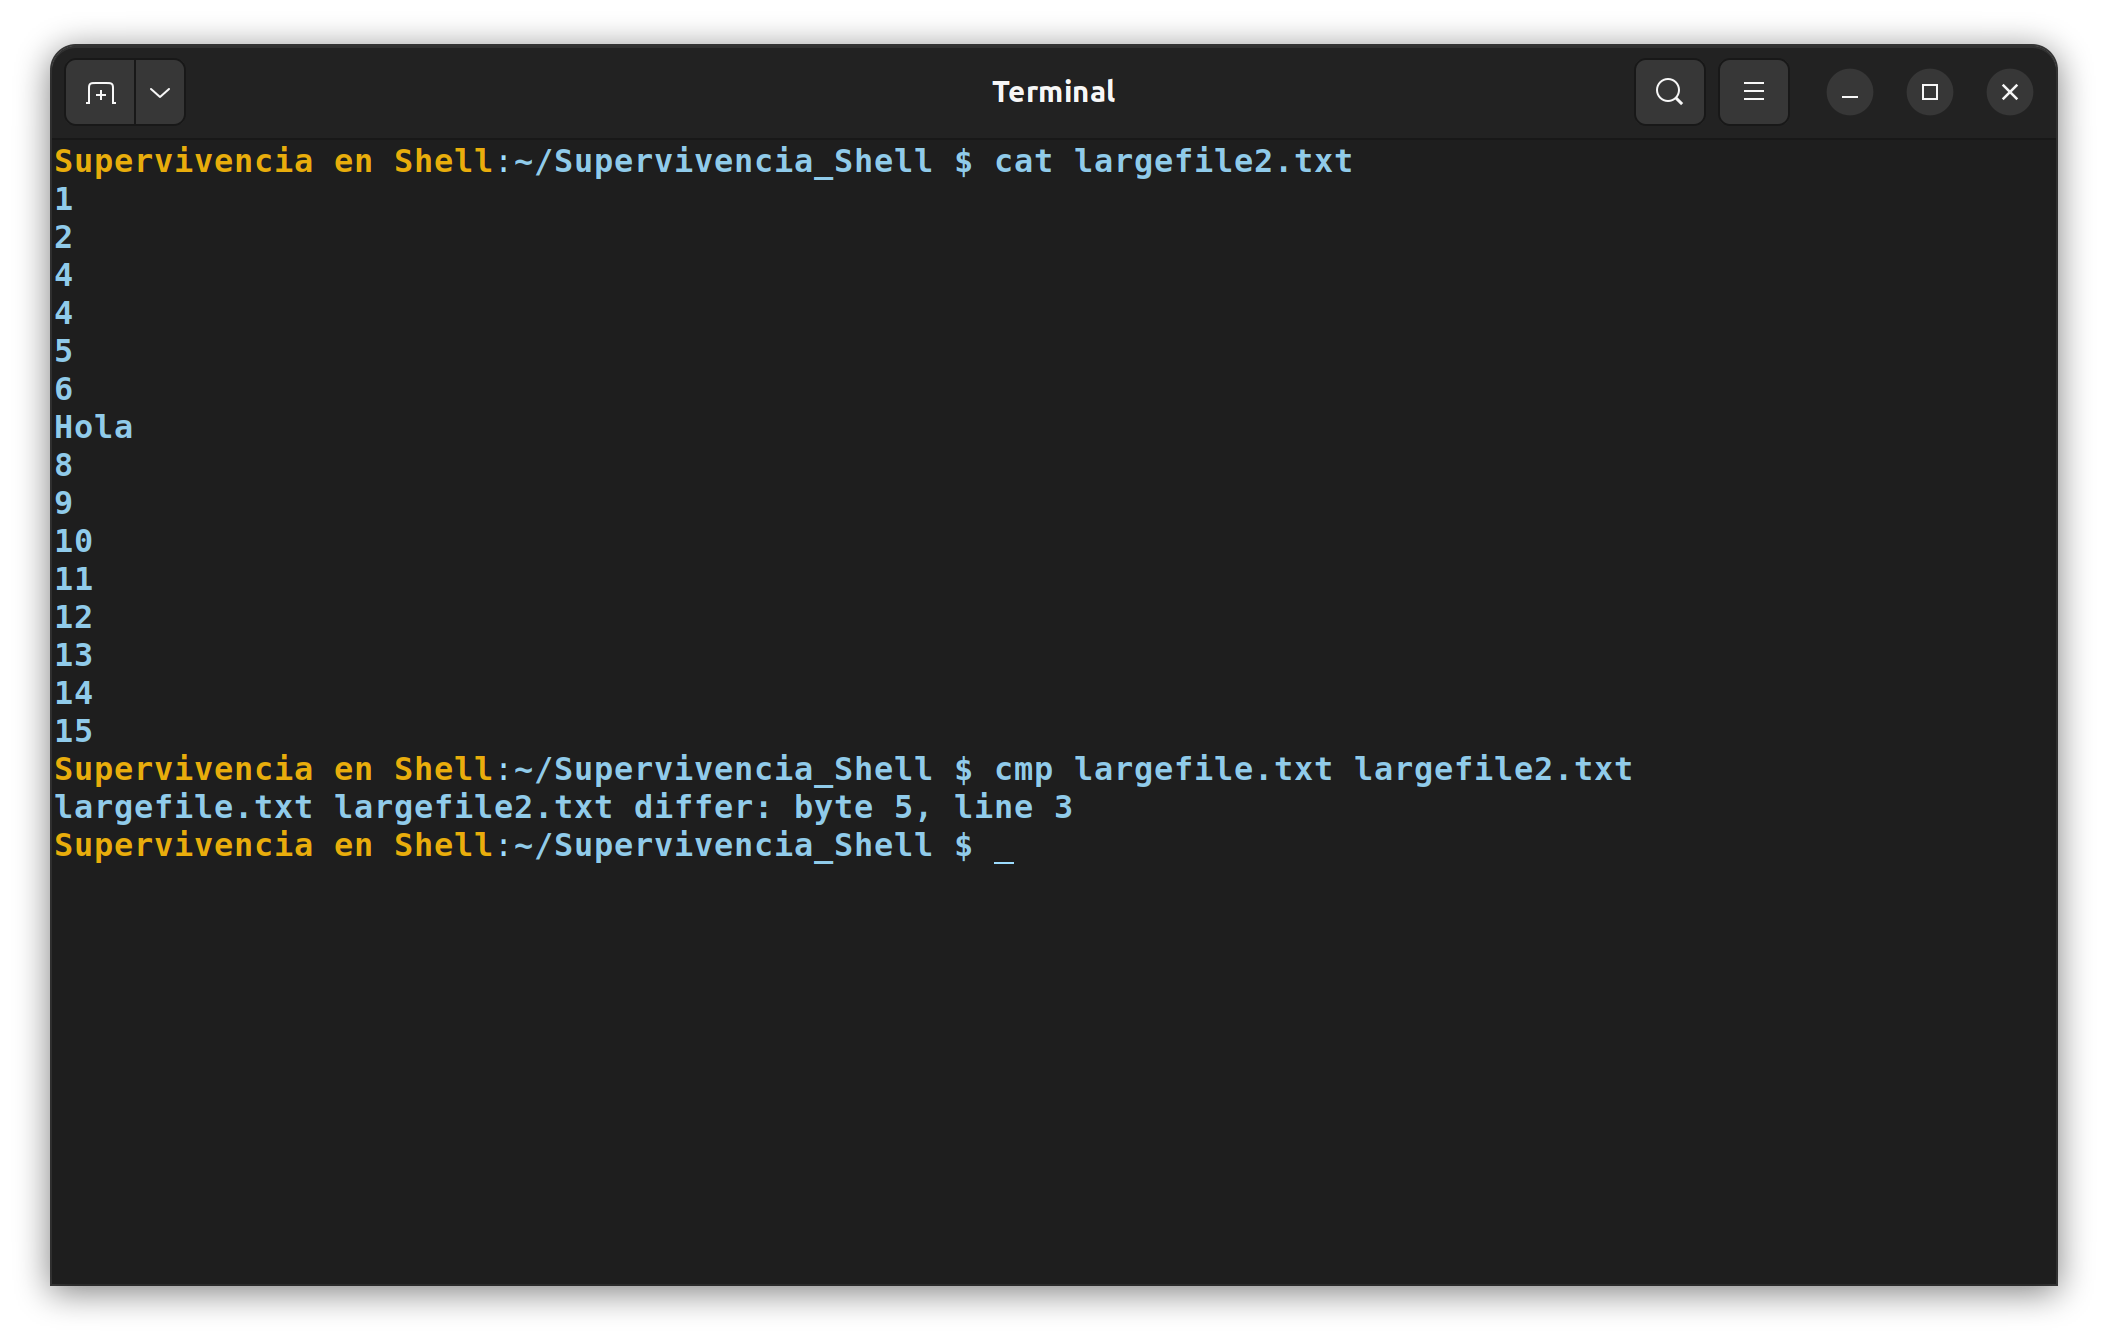
\includegraphics[width=0.75\textwidth]{cmp}
	\end{frame}
	
	\begin{frame}
		\frametitle{Comparando ficheros: diff}
		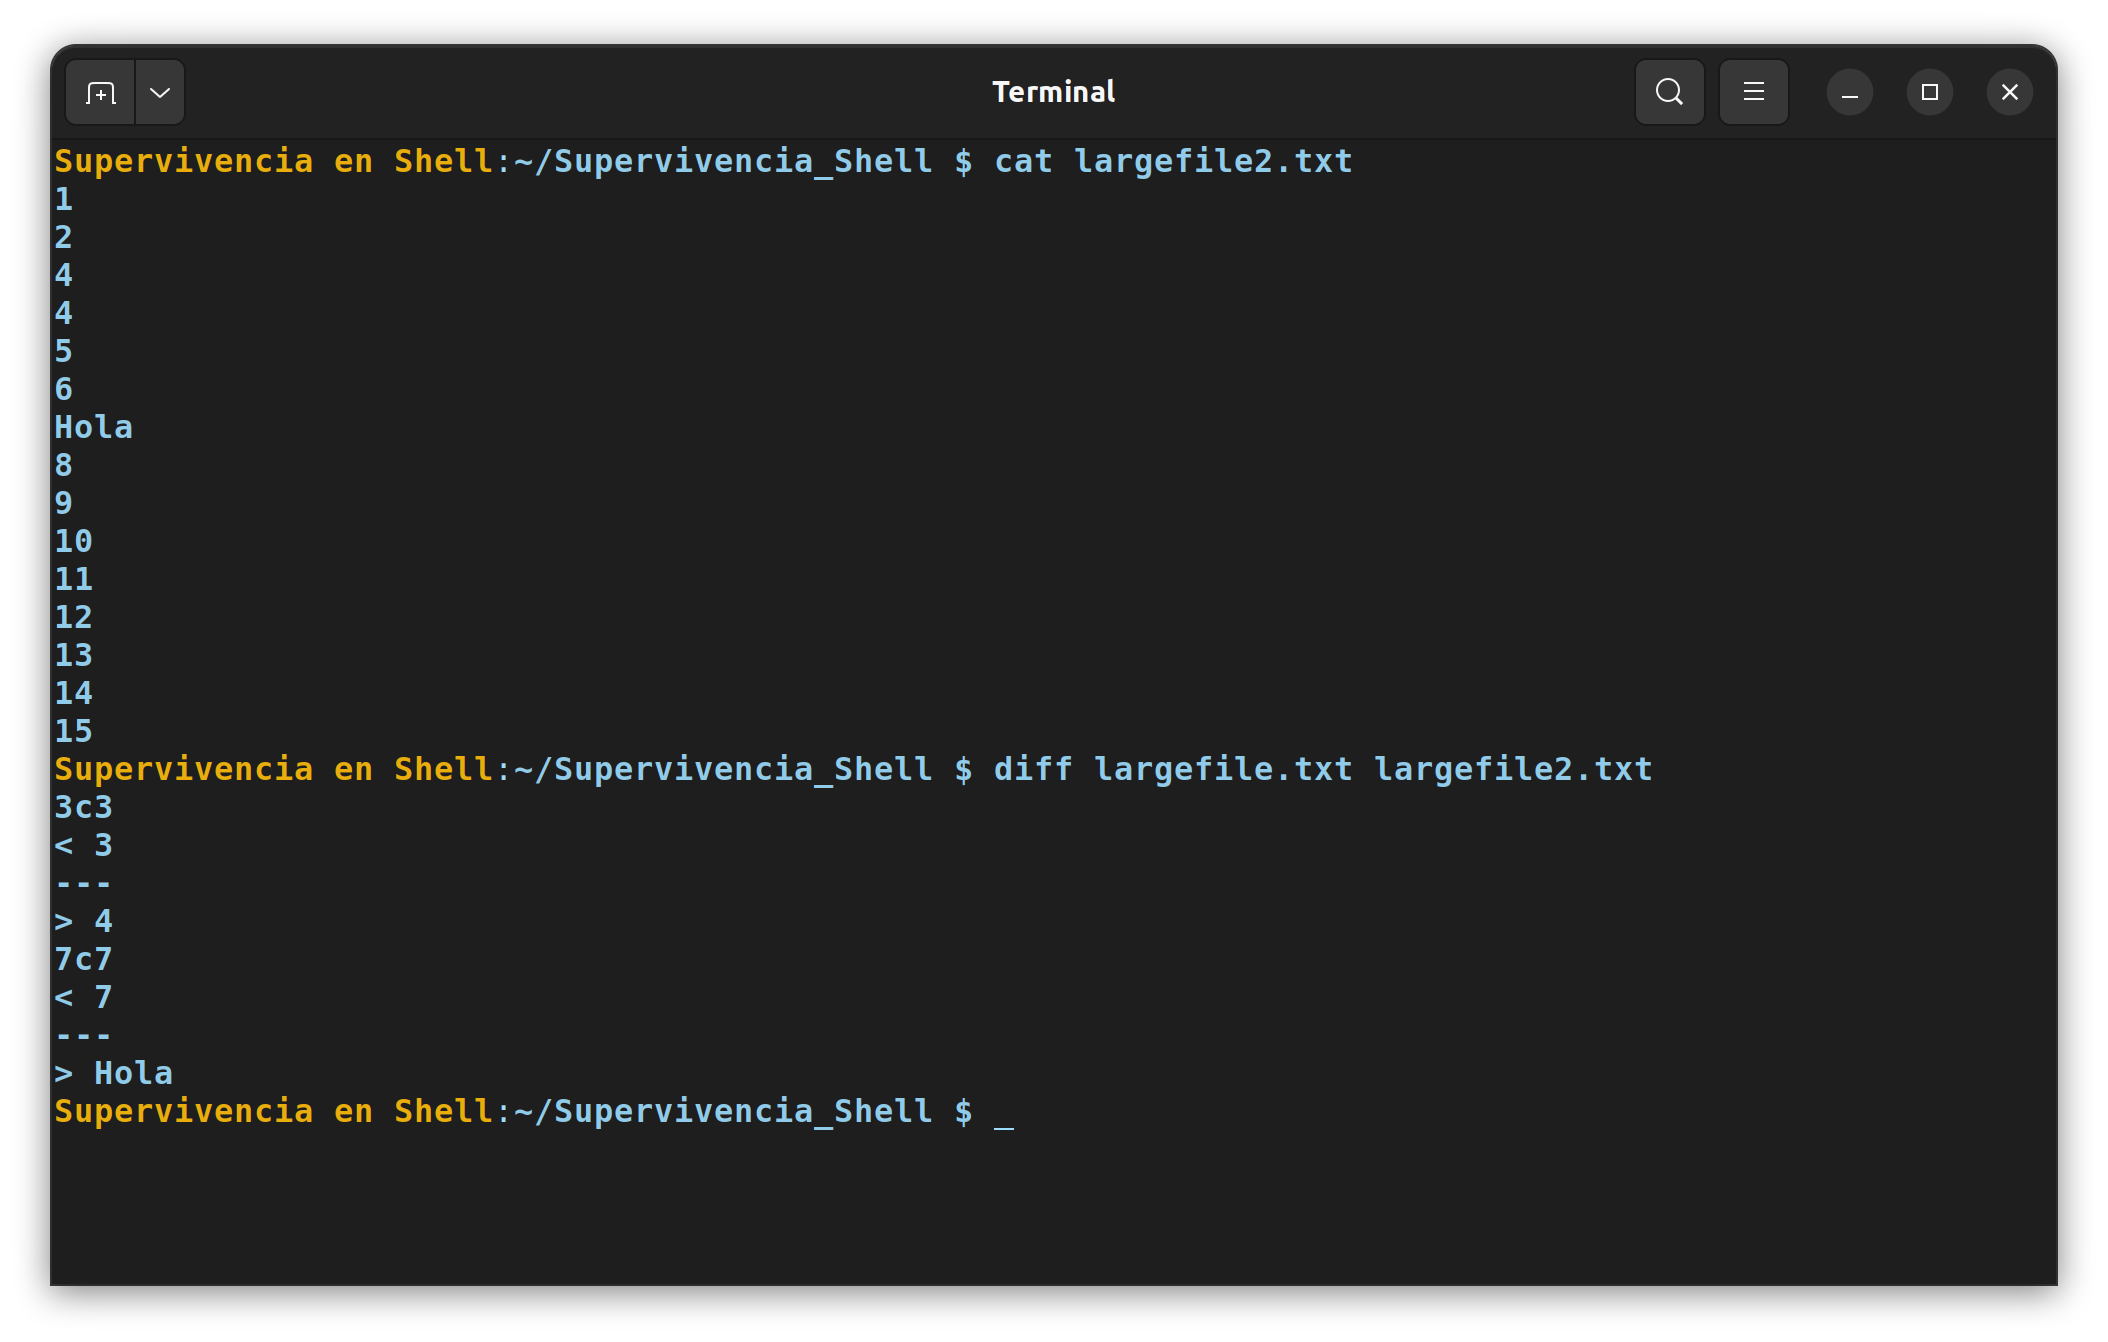
\includegraphics[width=0.75\textwidth]{diff}
	\end{frame}
			
	\begin{frame}
		\frametitle{Modificando ficheros: tar}
	\end{frame}
	
	\begin{frame}
		\frametitle{Modificando ficheros: gzip/gunzip}
	\end{frame}
		
	\begin{frame}
		\frametitle{Modificando ficheros: nano}
		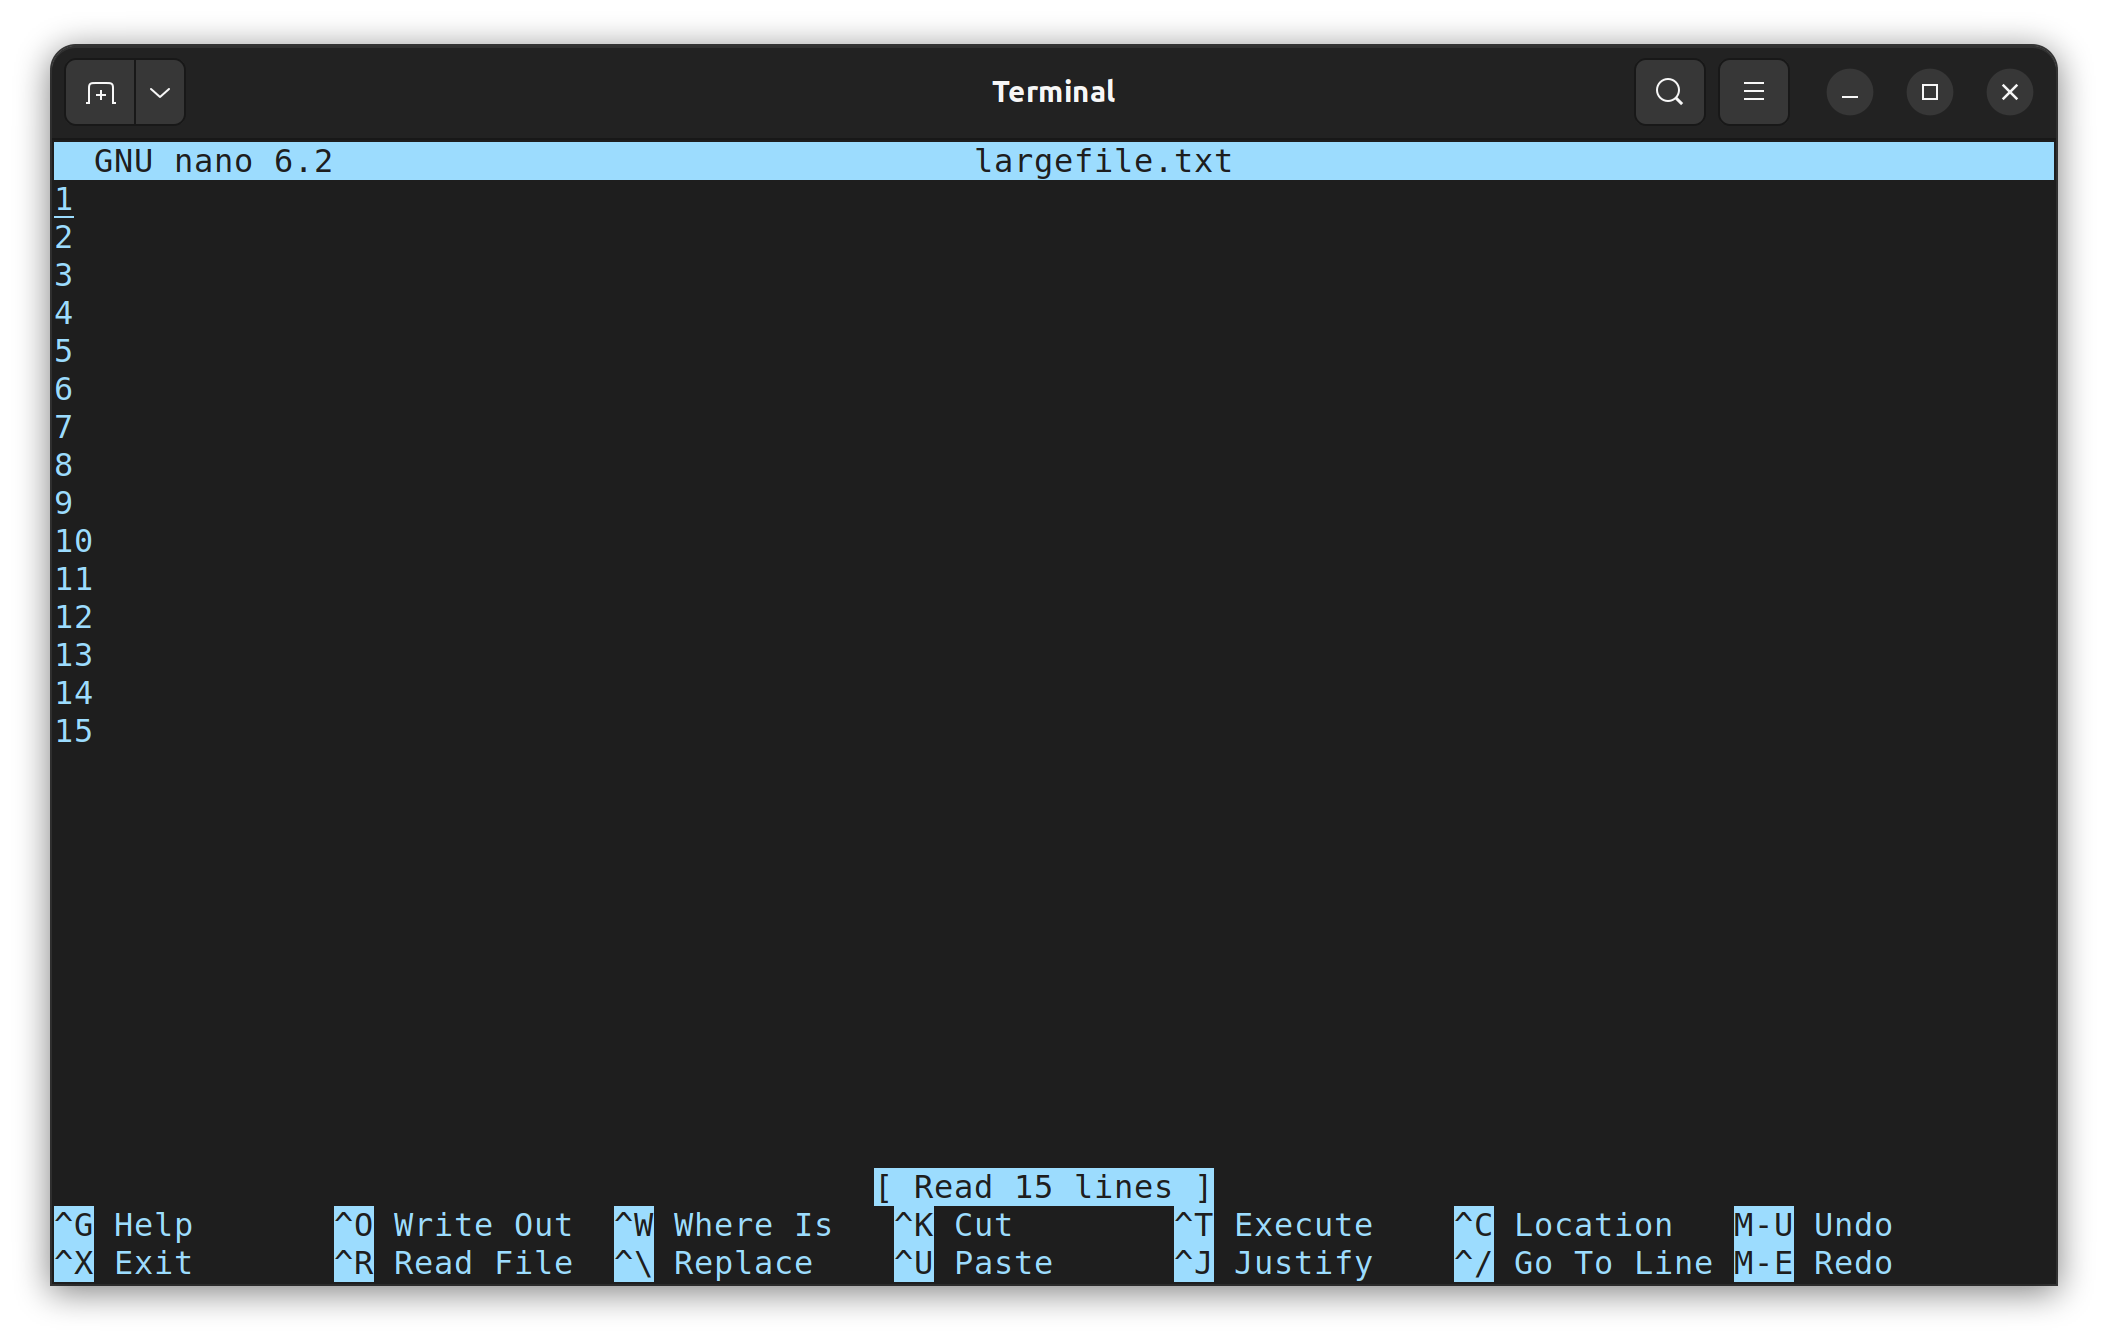
\includegraphics[width=0.75\textwidth]{nano}
	\end{frame}
	
	\begin{frame}
		\frametitle{Controlando el terminal: clear}
		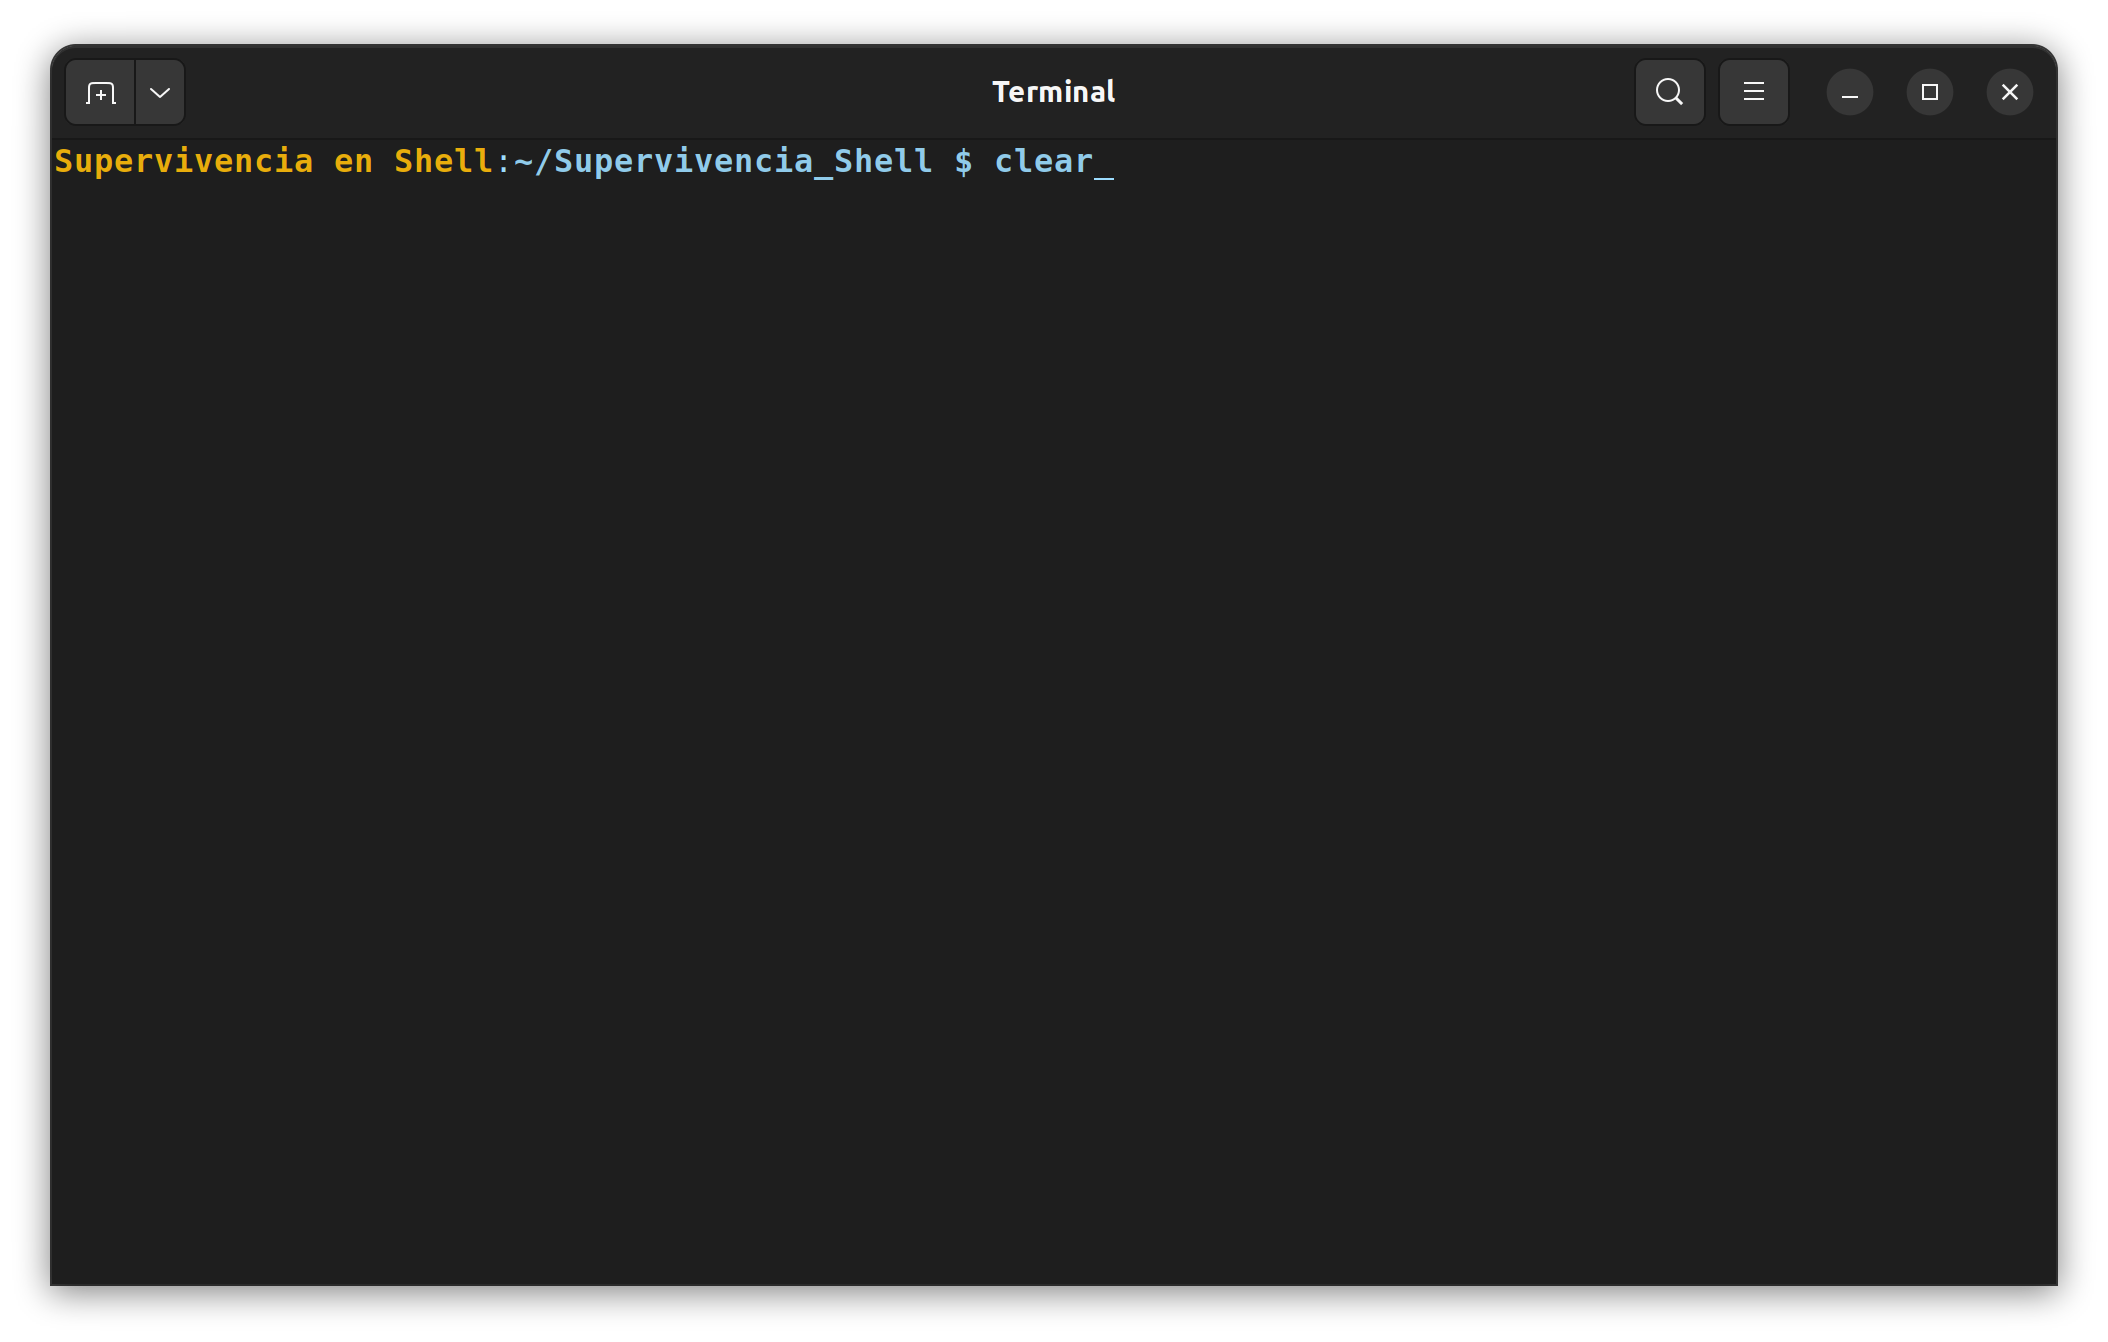
\includegraphics[width=0.75\textwidth]{clear}
	\end{frame}	
	
	\begin{frame}
		\frametitle{Controlando el terminal: reset}
		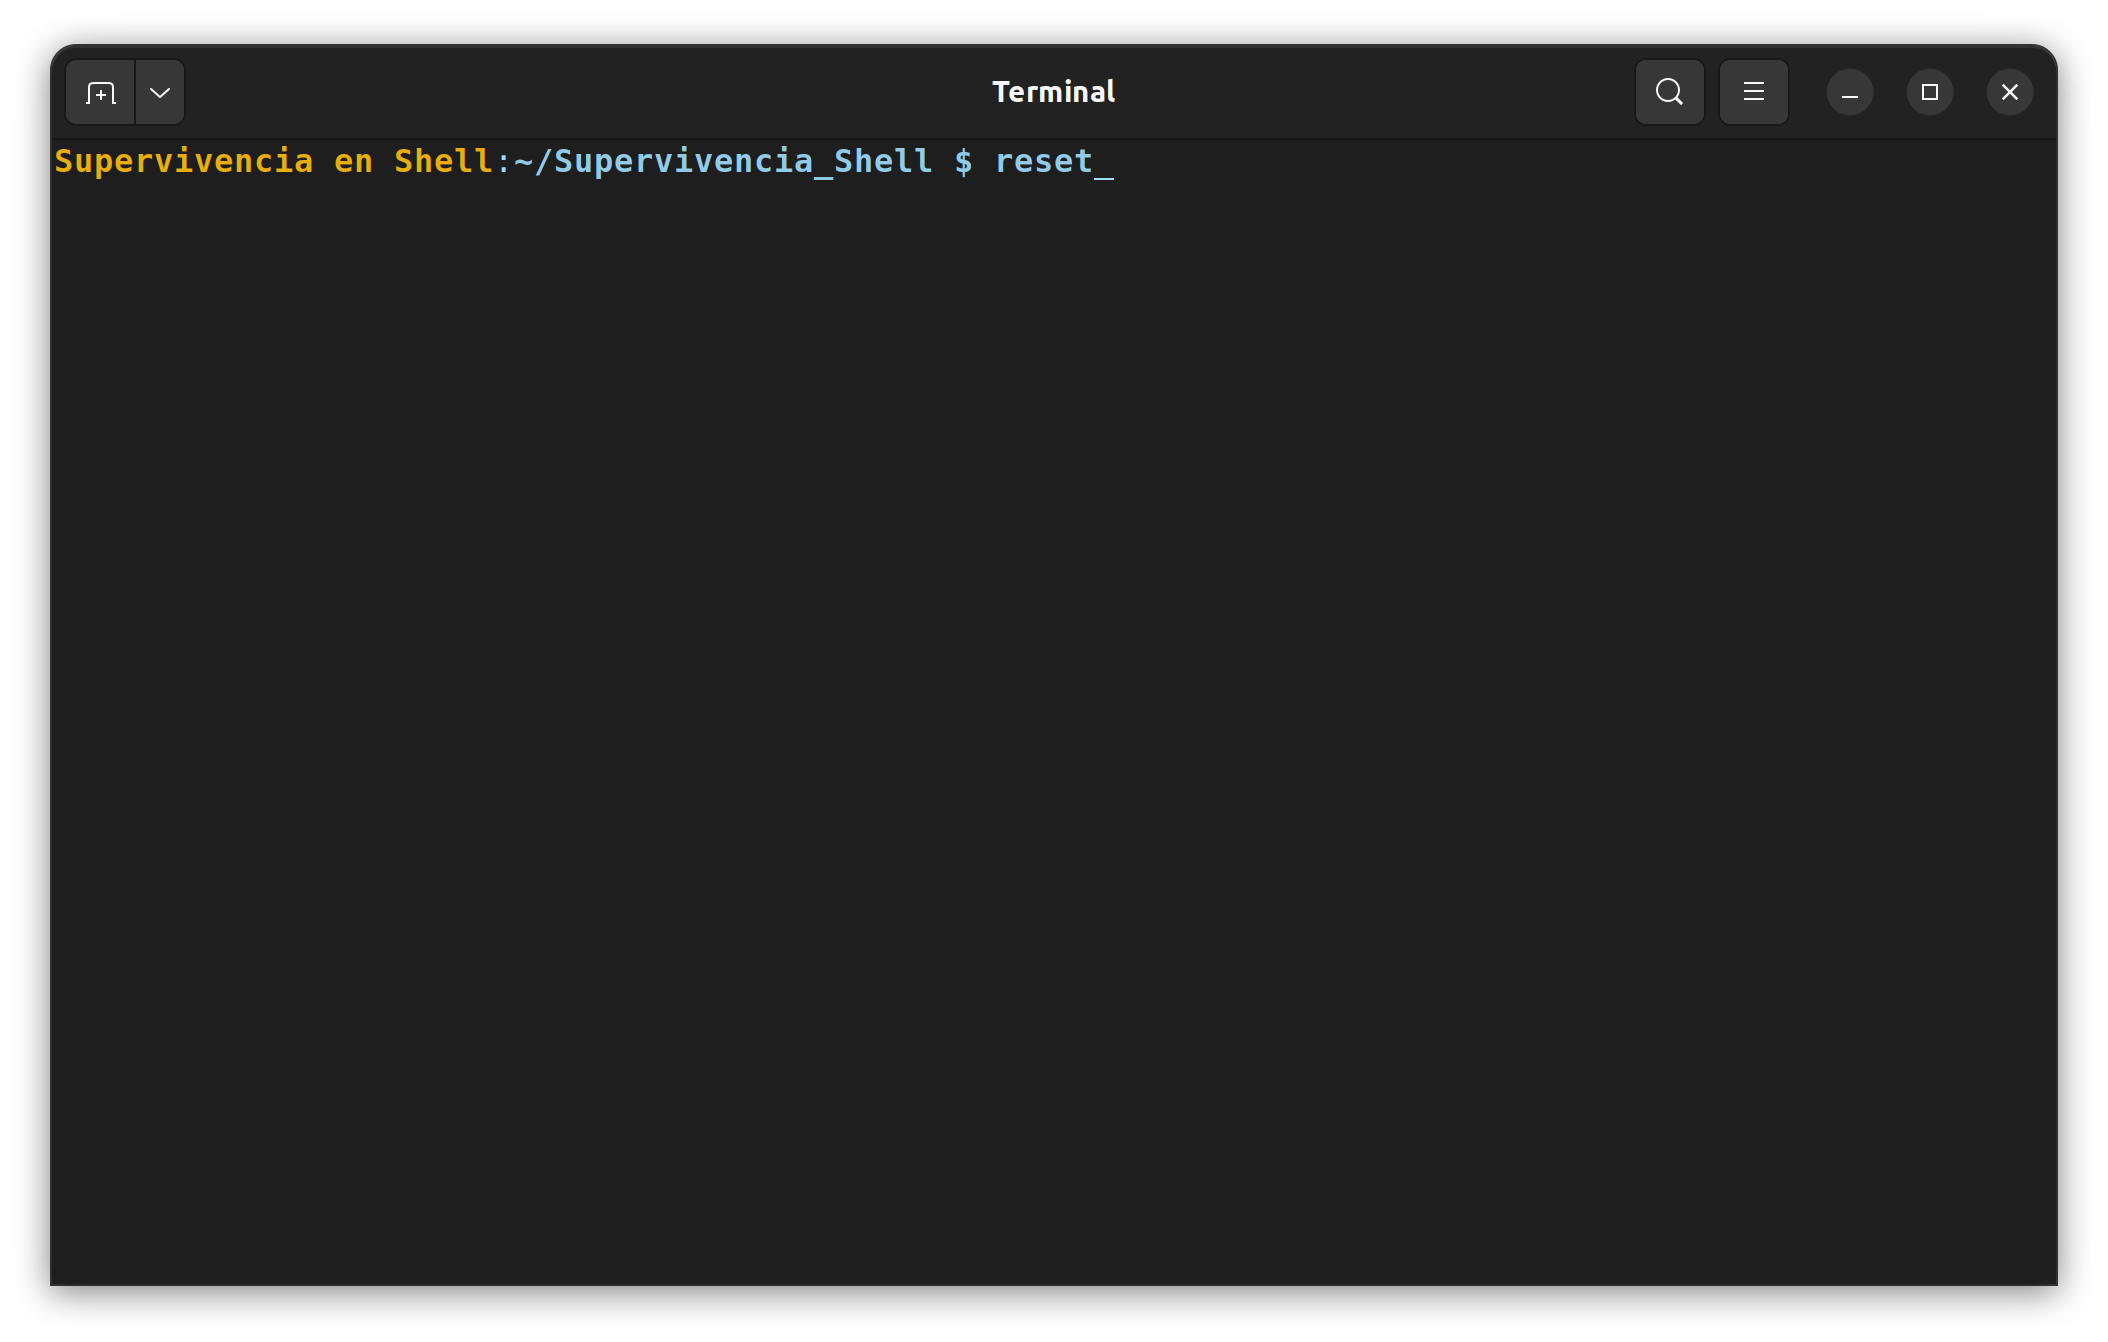
\includegraphics[width=0.75\textwidth]{reset}
	\end{frame}	
	
	\begin{frame}
		\frametitle{Controlando el terminal: exit}
		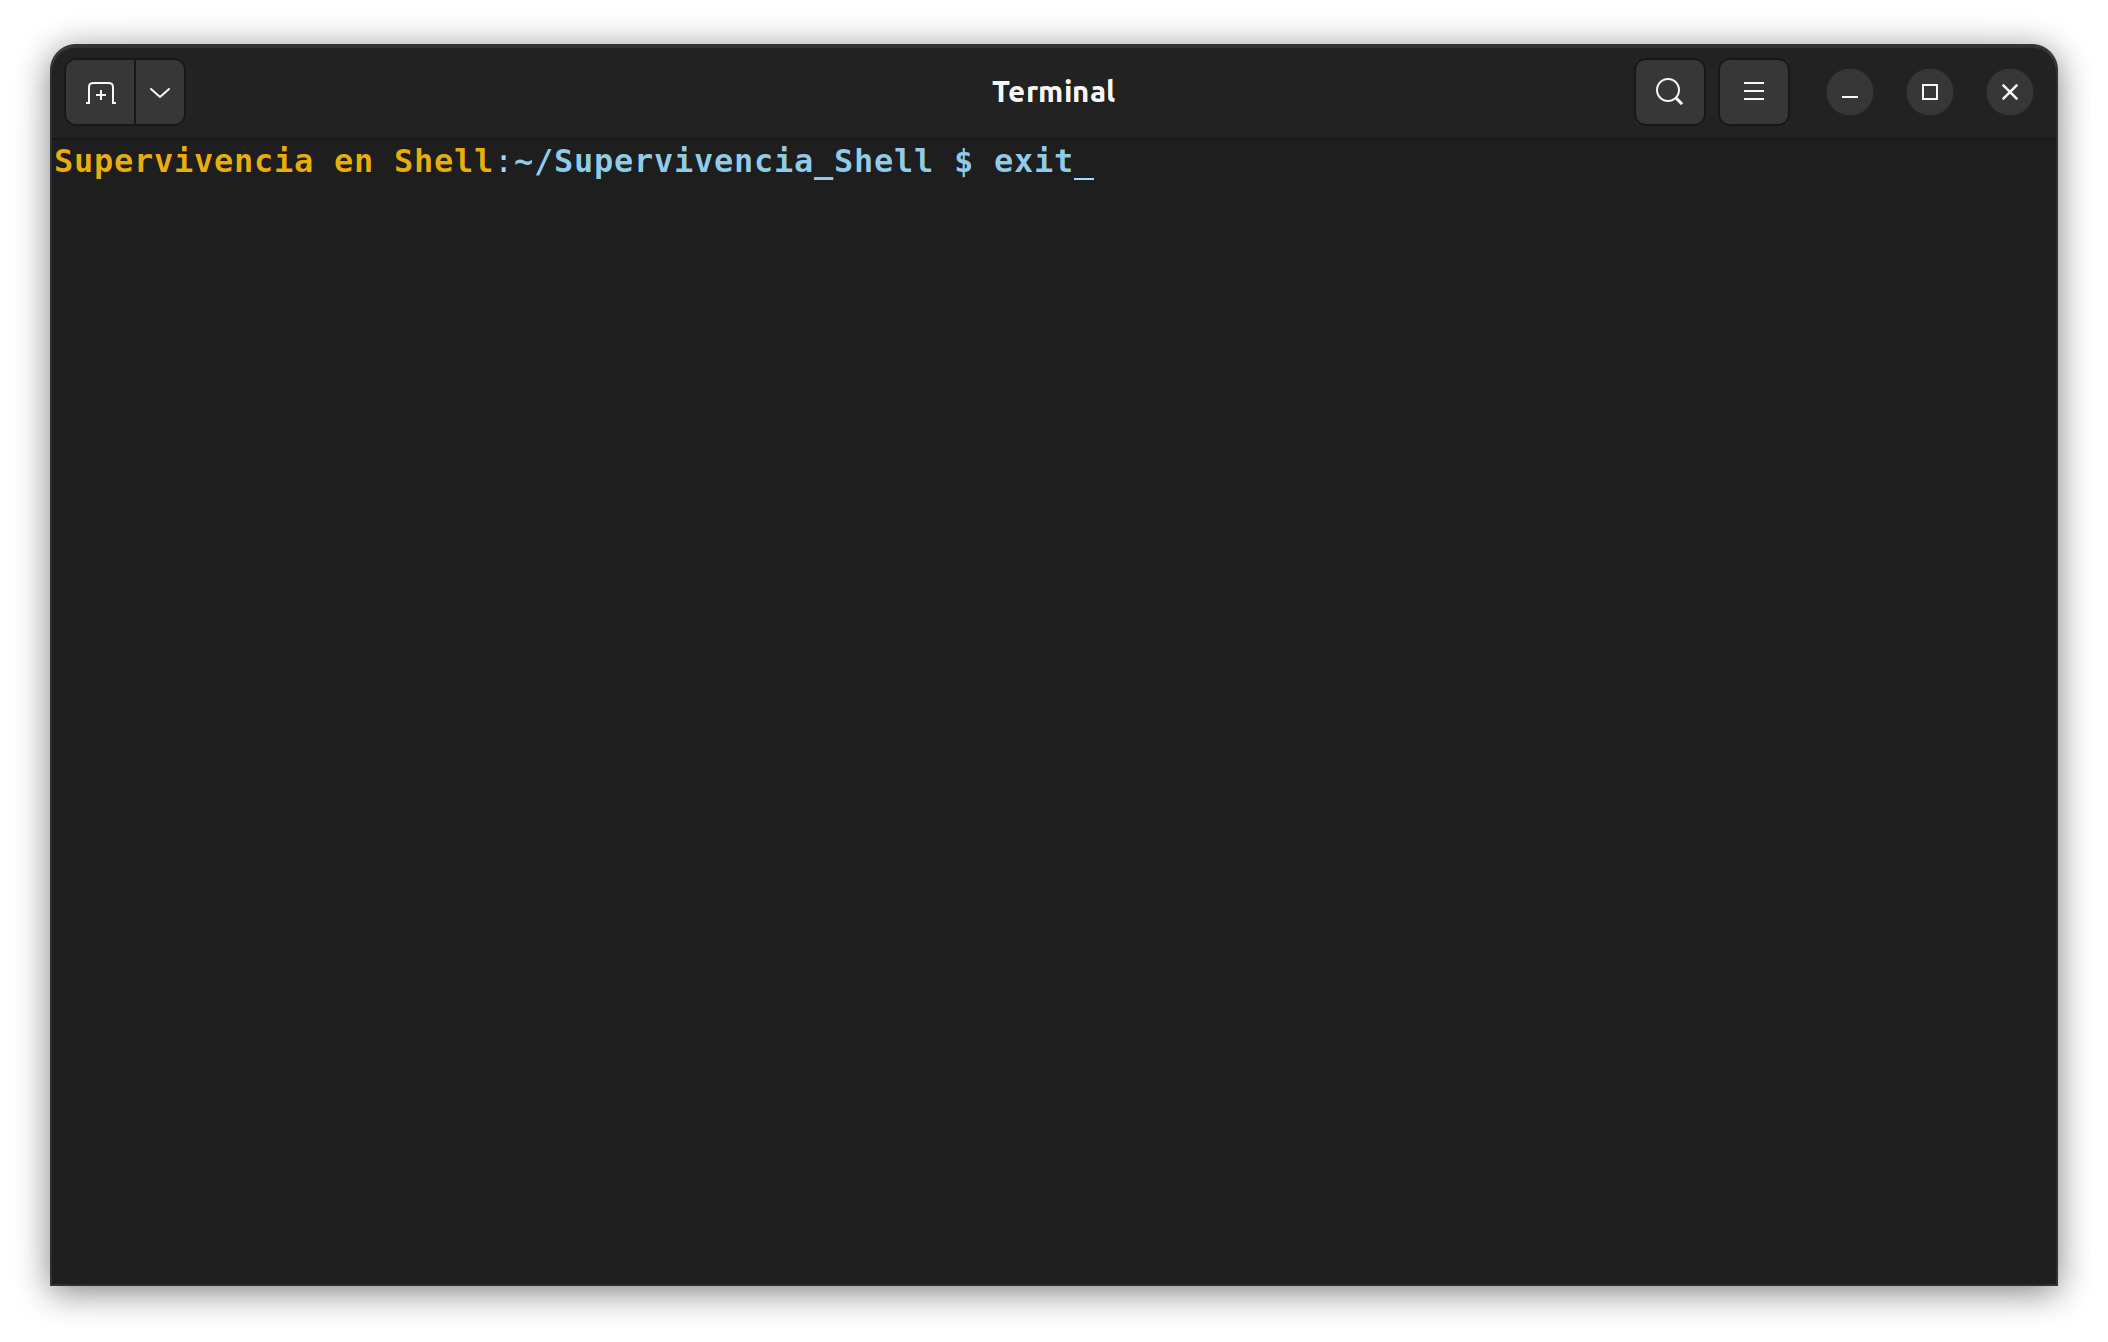
\includegraphics[width=0.75\textwidth]{exit}
	\end{frame}

	\begin{frame}
		\frametitle{Uso avanzado: alias}
	\end{frame}	

	\begin{frame}
		\frametitle{Uso avanzado: pipes}
	\end{frame}
	
	\begin{frame}
		\frametitle{Uso avanzado: redirecciones a ficheros}
	\end{frame}	
		
	\begin{frame}
		\frametitle{Extra: laburjc}
	\end{frame}
	
	\begin{frame}
		\frametitle{Menciones}
		\begin{itemize}
			\item Gorka Guardiola paurea@gmail.com
			
			\item Enrique Soriano enrique.soriano@urjc.es
		\end{itemize}
	\end{frame}
\end{document}